%\RequirePackage[l2tabu,orthodox]{nag}
\documentclass[a4paper,14pt,oneside,openany]{memoir}
% ,fleqn
% To have all equations flush left, add the fleqn option to your document class (or the packages that use it, like amsmath):
%%% Поля и разметка страницы %%%
\usepackage{geometry}   % Для последующего задания полей

%%% Математические пакеты %%%
\usepackage{amsthm,amsmath,amscd}    % Математические дополнения от AMS
\usepackage{amsfonts,amssymb}        % Математические дополнения от AMS
%\usepackage{mathtools}              % Добавляет окружение multlined
%\usepackage{xfrac}                  % Красивые дроби

\usepackage{xcolor}


%%% Кодировки и шрифты %%%

\usepackage{cmap}                    % Улучшенный поиск русских слов в полученном pdf-файле
\usepackage[T1,T2A]{fontenc}         % Поддержка русских букв

%%% Гиперссылки %%%

\usepackage[unicode]{hyperref}[2012/11/06]
\usepackage[russian]{cleveref}


% Реализация пакетом biblatex через движок biber

%%% Реализация библиографии пакетами biblatex и biblatex-gost с использованием движка biber %%%
\usepackage[autostyle]{csquotes}

\usepackage[%
backend=biber,% движок
bibencoding=utf8,% кодировка bib файла
sorting=none,% настройка сортировки списка литературы
% defernumbers=true, % откомментируйте, если требуется правильная нумерация ссылок на литературу в режиме черновика. Замедляет сборку
]{biblatex}[2016/09/17]%
\addbibresource{external.bib}


%%% Шаблон %%%
\DeclareRobustCommand{\fixme}{\textcolor{red}}  % решаем проблему превращения
%\newcommand{\fixme}{\textcolor{red}}  % решаем проблему превращения
% названия цвета в результате \MakeUppercase,
% http://tex.stackexchange.com/a/187930,
% \DeclareRobustCommand protects \fixme
% from expanding inside \MakeUppercase

%%% Макет страницы %%%
% Выставляем значения полей (ГОСТ 7.0.11-2011, 5.3.7)
\geometry{a4paper, top=2cm, bottom=2cm, left=2.5cm, right=1cm, nofoot, nomarginpar} %, heightrounded, showframe
\setlength{\topskip}{0pt}   %размер дополнительного верхнего поля
\setlength{\footskip}{12.3pt} % снимет warning, согласно https://tex.stackexchange.com/a/334346

%%% Интервалы %%%
%% По ГОСТ Р 7.0.11-2011, пункту 5.3.6 требуется полуторный интервал
%% Реализация средствами класса (на основе setspace) ближе к типографской классике.
%% И правит сразу и в таблицах (если со звёздочкой)
%\DoubleSpacing*     % Двойной интервал
\OnehalfSpacing*    % Полуторный интервал
%\setSpacing{1.42}   % Полуторный интервал, подобный Ворду (возможно, стоит включать вместе с предыдущей строкой)

%%% Выравнивание и переносы %%%
%% http://tex.stackexchange.com/questions/241343/what-is-the-meaning-of-fussy-sloppy-emergencystretch-tolerance-hbadness
%% http://www.latex-community.org/forum/viewtopic.php?p=70342#p70342
\tolerance 1414
\hbadness 1414
\emergencystretch 1.5em % В случае проблем регулировать в первую очередь
\hfuzz 0.3pt
\vfuzz \hfuzz
%\raggedbottom
%\sloppy                 % Избавляемся от переполнений
\clubpenalty=10000      % Запрещаем разрыв страницы после первой строки абзаца
\widowpenalty=10000     % Запрещаем разрыв страницы после последней строки абзаца
\brokenpenalty=4991     % Ограничение на разрыв страницы, если строка заканчивается переносом

%%% Оглавление %%%
\renewcommand{\cftchapterdotsep}{\cftdotsep}                % отбивка точками до номера страницы начала главы/раздела


\AtBeginDocument{%
	\setlength{\parindent}{2.5em}                   % Абзацный отступ. Должен быть одинаковым по всему тексту и равен пяти знакам (ГОСТ Р 7.0.11-2011, 5.3.7).
}

\usepackage{cmap}   % Улучшенный поиск русских слов в полученном pdf-файле
    \usepackage[T1,T2A]{fontenc}                    % Поддержка русских букв

  
\renewcommand{\chaptername}{Глава}


\begin{document}
	
% Титульный лист (ГОСТ Р 7.0.11-2001, 5.1)
\thispagestyle{empty}
\begin{center}
Федеральное государственное бюджетное учреждение науки <<Институт прикладной механики Российской академии наук <<ИПРИМ РАН>>
\end{center}
%
\vspace{0pt plus4fill} %число перед fill = кратность относительно некоторого расстояния fill, кусками которого заполнены пустые места
\begin{flushright}
	На правах рукописи
	
	%\textsl {УДК \thesisUdk}
\end{flushright}          % Титульный лист
\tableofcontents*
\chapter{Обзор существующей проблемы}\label{ch:overview:1}

\section{Обзор современного состояния и ключевых проблем проектирования, потенциальных решений для конструкций резервуаров для хранения криогенного жидкого водорода для применения в авиации}\label{ch:overview:1:sec1}
% https://ntrs.nasa.gov/api/citations/20060056194/downloads/20060056194.pdf

\subsection{Абстракт}\label{ch:overview:1:sec1:sub1}

Благодаря высокой удельной энергоемкости жидкий водород (\(LH_2\) --- liquid hydrogen~\(H_2\)) выделяется на горизонте альтернативных источников энергии для будущих летательных аппаратов. Как следствие, существует потребность в системах хранения водорода, которые должны обеспечивать достаточную вместимость для полетов продолжительностью от нескольких минут до нескольких дней. Понятно, что разработка большого, легкого, многоразового криогенного резервуара для хранения водорода имеет решающее значение для достижения целей и обеспечения топливом летательных аппаратов на водороде, особенно для длительных полетов. В данной работе  представлен обзор текущего состояния дел в области материалов, конструкций и систем изоляции криогенных резервуаров ---- наряду с попыткой определения ключевых проблем  разработки легкой и долговременной системы хранения \(LH_2\). Рассмотренные широкие классы изоляционных систем включают пенопласты (включая современные аэрогели) и системы многослойной изоляции (МСИ -- MLI --- multilayer insulation) с вакуумом. Системы МСИ показывают перспективность для долгосрочного применения. Рассмотренные структурные конфигурации включают одно- и двустенные конструкции, в том числе многослойные конструкции. Потенциальными кандидатами для материала стенок являются монолитные металлы, а также полимерные матричные композиты и прерывисто армированные металлические матричные композиты. Для применения в кратковременных полетах может быть достаточно простых конструкций баков. В качестве альтернативы для более длительных полетов наиболее оптимальной представляется конструкция с двойными стенками и вакуумной системой изоляции. Современные тенденции в разработке материалов для обшивки рассматриваются в случае, когда обшивка требуется для минимизации или устранения потерь водородного топлива через проницаемость.


Интерес к разработке летательных аппаратов, использующих альтернативные источники энергии, такие как водород, обусловлен прежде всего тем, что водород обеспечивает низкий или нулевой выброс в окружающую среду вредных продуктов. Среди рассматриваемых вариантов применения -- продолжительность полета, которая может составлять от нескольких минут до многих дней. Как пример, вот пример современного беспилотного летательного аппарата (БПЛА)  NASA с большой продолжительностью полета: Helios~HP03, БПЛА на солнечных батареях, использующий систему регенеративных топливных элементов для накопления энергии. Он был способен летать в течение месяца, но имел ограниченную грузоподъемность 230 кг (550 фунтов), которая должна была распределяться по крыльям, и мог летать на пиковой высоте около 21 км (70 000 футов).

В коммерческих самолетах продолжительность полета, скорее всего, будет составлять порядка нескольких часов. Стремление к увеличению грузоподъемности и продолжительности полета требует использования силовой установки с более высокой удельной мощностью и повышенной общей эффективностью. Исследуемые в настоящее время системы включают использование топливных элементов с электродвигателями и двигателями внутреннего сгорания. Текущие предварительные требования к программам, которые стимулируют разработку водородных самолетов с большой продолжительностью полета, включают продолжительность полета 14 дней (336 часов) с полезной нагрузкой, достаточной для размещения приборов.

Водород обладает наибольшей энергией на единицу массы среди различных видов жидкого и газообразного топлива, как отмечает Томас (\cite{thomas}). Водород, хранящийся в жидком виде, значительно увеличивает энергию на единицу объема по сравнению с газообразным водородом (\(GH_2\) --- gaseous hydrogen). Газообразный водород, хранящийся при давлении 35~МПа~(5~ksi) и температуре \(20^{\circ} C \,(68^{\circ} F)\), хранит только одну треть энергетического содержания на единицу объема жидкого водорода (\(LH_2\)), как показано Томасом. Хотя для хранения (\(LH_2\)) при низком давлении и криогенной температуре требуется изоляция, она меньше, чем при хранении  (\(GH_2\)) при высоком давлении. Другой метод хранения водорода в компактной и безопасной форме --- это гидрид металла. К сожалению, использование гидридов металлов накладывает ограничение, связанное с чрезмерным весом, что исключает их использование в чувствительных к весу приложениях. 

В настоящее время применение криогенных резервуаров для хранения в аэрокосмической отрасли, где вес имеет первостепенное значение, ограничено короткими полетами, например, на космических ракетах-носителях. 
Криогенные жидкости переливаются в баки для хранения транспортного средства непосредственно перед запуском, а большая часть жидкостей расходуется во время выхода на орбиту, в течение нескольких минут. 
Криогенные жидкости исчерпываются со скоростью, при которой выкипание не представляет значительной проблемы (\( {\color{red} \text{уточнить у кого-нибудь, кто в теме}} \)). В таких случаях для резервуаров обычно достаточно легкой пенопластовой изоляции. 
В глубоком космосе теплопередача к криогенной жидкости значительно меньше, чем в условиях окружающей среды на поверхности Земли, что снижает необходимость в сверхнизкой проводимости и толстой изоляции. Именно для самолетов с относительно большой продолжительностью полета порядка нескольких дней возникают наибольшие инженерные трудности при разработке долговременных и легких систем хранения водорода.

Необходимость снижения веса в сочетании с хорошими изоляционными свойствами для долгосрочного хранения представляет собой новую задачу в проектировании криогенных резервуаров. Это дает возможность применить более современные материалы и конструктивные идеи в попытке снизить общий вес и сохранить объем на приемлемом и практичном уровне.

В данном работе рассматриваются конструктивные и тепловые элементы системы баков для хранения криогенных веществ для летательного аппарата. В следующих разделах будут рассмотрены отдельные компоненты системы баков. 

После подробного описания основных проблем в следующих разделах будут рассмотрены подкомпоненты системы баков. Также будут рассмотрены материалы и их термическая и химическая совместимость со средами, в которых работает система хранения \(LH_2\). Будут рассмотрены методы строительства резервуара. Сюда входит оценка металлических и полимерно-матричных композитных (ПМК) материалов и архитектуры, используемой для создания резервуара. Также будет обсуждаться возможность использования футеровки ({\color{green}  Футеровка (нем. Futter «подкладка, подбой») -- облицовка огнеупорными, химически стойкими, износостойкими, а также теплоизоляционными материалами, которым покрывается внутренняя поверхность металлургических печей, ковшей, топок котлов и прочего оборудования. Футеровка производится для обеспечения защиты поверхностей от возможных механических, термических, физических и химических повреждений.}).

Другие важные области конструкции бака, включая методы крепления для интеграции системы бака с планерной рамой, ребра жесткости, перегородки для выброса топлива и порты, подробно не рассматриваются, поскольку они выходят за рамки данного отчета.

Методы изоляции будут рассмотрены для определения оптимальной системы для применения в летательных аппаратах. 

\section{Ключевые проблемы разработки}\label{ch:overview:1:sec2}

Успешная реализация будущих легко-весных и экологически чистых ЛА требует объединения ряда инновационных и передовых технологий, а также разработки новых технических средств и технологий их производства. Как уже упоминалось выше, особый интерес представляют ЛА на водородном топливе с продолжительностью полета в несколько дней. Водород можно хранить как в газообразной, так и в жидкой форме. Газообразный водород требует в \(5.6\) раз большего объема по сравнению с жидкой форме, при этом жидкий водород хранится под давлением примерно \(163\) атм (\(2400\) фунтов на кв. дюйм) и при температуре \(15^{\circ}C (60^{\circ}F)\).

Необходимый при этом чрезмерный объём, вес бака и проблемы связанные с обеспечением безопасности, при с хранением водорода под высоким давлением, исключают использование газообразного водорода \(GH_2\) в качестве топлива для данного применения. В качестве альтернативы, гидриды металлов могут компактно и безопасно хранить водород, хотя эти системы будут слишком тяжелыми и, следовательно, непрактичными. Кроме того, для <<перезарядки>> большинства металлогидридных систем потребуются дни или даже недели. Гидриды \(MgNi\) могут достичь приблизительно 5 процентов водорода по весу, но требуют более высоких температур для активации кристаллического слоя.

Проблемы металлогидридов были обобщены Брюером (\cite{brewer1991}), который отметил их непрактичность для авиационных применений. Жидкий водород в насыщенном состоянии является жизнеспособным вариантом для самолетов с большой продолжительностью полета. Однако проектирование криогенного резервуара для хранения \(LH_2\), в сочетании с использованием \(LH_2\) в качестве авиационного топлива, сопряжено со многими проблемами. Некоторые из ключевых проблем, включая геометрию, температуру, проницаемость, водородное охрупчивание и факторы безопасности, кратко обсуждаются ниже.

\subsection{Реальные размеры, геометрия}\label{ch:overview:1:sec2:sub1}

Несмотря на то, что жидкий водород \(LH_2\) имеет высокую температуру сгорания, его низкая плотность в сочетании с потенциально большой продолжительностью полета и использованием нерекуперативной системы хранения может привести к необходимости бака большого объема.

Неинтегральный (т.е. не являющийся частью конструкции летательного аппарата) большой бак означает большую лобовую (поперечную) площадь и площадь поверхности, что приведет к увеличению сопротивления. Для успешных конфигураций потребуются инновационные конструкции с малой лобовой площадью и площадью поверхности.

Интеграция большого бака в ЛА сама по себе является серьезной проблемой. Интегральные баки, напротив, требуют сложной конструкции и создают множество производственных проблем. Интегральные баки являются конструктивным элементом ЛА, т.е. воспринимают нагрузки на фюзеляж, а также обеспечивают сохранность топлива. Неинтегральные баки служат только в качестве контейнеров для топлива и устанавливаются внутри корпуса ЛА и удерживаются им (\cite{brewer1991}). Как упоминалось ранее, неинтегральные баки не обязательно должны соответствовать форме ЛА; их конструкция может быть относительно простой, например, сферической или цилиндрической. Баки сферической формы обеспечивают минимальную площадь поверхности для данного объема, поэтому пассивное нагревание бака может быть сведено к минимуму, что минимизирует выкипание LH2. Однако сферическая форма создает некоторые специфические производственные трудности и имеет большую площадь фронтальной поверхности, что приводит к увеличению силы сопротивления по сравнению с баком цилиндрической формы. В качестве альтернативы, цилиндрические формы проще в изготовлении, но имеют более высокое отношение площади поверхности к объему, что приводит к более высокой пассивной тепловой нагрузке на бак.

\subsection{Криогенные температуры}\label{ch:overview:1:sec2:sub2}

Нормальная температура кипения \(LH_2\) составляет \(-252^{\circ}C (-423^{\circ}F)\). \(LH_2\) необходимо держать ниже этой температуры, чтобы минимизировать выкипание, то есть потерю топлива и повышение давления в баке. Во время наземных операций максимальная разница температур внутри и снаружи конструкции бака может достигать \(\Delta T = 300^{\circ}C~(540^{\circ}F)\). Для поддержания такого большого температурного градиента, очевидно, необходима легковесная изоляция с низкой теплопроводимостью. Как уже упоминалось, большинство предыдущих применений криогенного топлива, такого как \(LH_2\), было ограничено короткой продолжительностью в несколько минут, как в ракетах-носителях, где проблема выкипания топлива не является критической. Однако для полетов большой продолжительности чрезмерное выкипание топлива очень нежелательно и ограничивает продолжительность полета летательного аппарата. Следовательно, количество пассивного тепла, которое поступает в бак и вызывает выкипание жидкого водорода, должно быть ограничено. Хранение \(LH_2\) на земле имеет аналогичные проблемы и требует специализированного оборудования и процедур для работы с ним. Установлено, что если поддерживать постоянное абсолютное давление \(LH_2\) на уровне примерно \(170 кПа (25 psia)\), то выкипание будет поддерживаться на приемлемом уровне и без лишних весовых нагрузок на конструкцию резервуара (\cite{brewer1991}). Кроме того, резервуар и любые соединительные трубопроводы или приспособления должны быть полностью изолированы от внешней атмосферы, поскольку все газы, за исключением гелия, застывают при температурах LH2 и повышают вероятность образования закупорки проточных трубопроводов и других компонентов.

\subsection{Проницаемость}\label{ch:overview:1:sec2:sub3}

Поскольку молекулы водорода очень малы, они чрезвычайно легко проникают через стенку резервуара. Проницаемость водорода является, пожалуй, самым критическим моментом в конструкции резервуара. Металлические баки являются очевидным решением этой проблемы, поскольку водород проникает через металлы медленнее, чем сквозь неметаллические материалы. Однако для летательного аппарата масса металлического бака может ограничить его грузоподъемность и продолжительность полета. Бак из композита с полимерной матрицей (КПМ --- PMC polymer matrix composite) с тонкой металлической обшивкой также решил бы проблему проницаемости, но вес все еще может оказаться проблемой. Кроме того, несоответствие коэффициента теплового расширения (КТР) между стенкой композитного бака и металлическим вкладышем приведет к их неравномерному сжатию, что, в результате, может вызвать напряжения в материале, которые могут привести к отслойке вкладыша от бака и/или его разрушению, что делает такую конструкцию нежелательной. 

Исследования проницаемости водорода, проведенные в ходе программы "Национальный аэрокосмический самолет" ( National Aerospace Plane program), были обнадеживающими, и было показано, что композитные баки без какого-либо вкладыша достаточно непроницаемы. Однако разрушение бака КПМ \(LH_2\) демонстрационного проекта X-33 во время наземных испытаний было вызвано микротрещинами полимерной матрицы в композитной внутренней оболочке конструкции бака (\cite{grimsley2001}). Микротрещины в композите возникли в результате несоответствия КТР углеродного волокна и полимерной матрицы в сочетании с большой разницей между температурой использования и температурой изготовления композита. Микротрещины создавали путь для утечки или проникновения водорода под давлением через стенку и проникновения в сотовый заполнитель. При нагревании трещины в матрице закрывались, жидкость испарялась, а образовавшиеся газы, которым некуда было выходить, вызывали повышение давления и в конечном итоге отслоение сердечника от внутренней композитной оболочки.  В последнее время были проведены исследования по оценке полимерных пленок и покрытий, которые можно было бы нанести на внутреннюю композитную оболочку и использовать в качестве барьера для удержания \(LH_2\) в резервуаре. Изготовление легких и непроницаемых резервуаров из современных материалов для криогенного применения является сложной задачей.

\subsection{Водородное охрупчивание}\label{ch:overview:1:sec2:sub4}

Многие материалы при воздействии водорода в больших концентрациях становятся хрупкими. Влияние водорода на поведение материалов хорошо описано (например, \cite{moodythompson1990}). Это один из видов разрушения материала. Когда материал становится более хрупким, его несущая способность и пластичность снижаются. Таким образом, могут произойти катастрофические разрушения без значительной деформации или видимого деградирования детали конструкции. Это ограничивает применение многих современных материалов в строительстве стенки резервуара.

Для решения этих проблем необходимы прорывные технологии в области материалов. Для возникновения водородного охрупчивания необходимы растягивающие напряжения, восприимчивый к воздействию водорода материал и присутствие водорода. Водородное охрупчивание может привести к образованию трещин при уровнях напряжения значительно ниже предела текучести. Хотя водородное охрупчивание больше всего зафиксировано для высокопрочных сталей, все материалы обладают определенной степенью восприимчивости. Устойчивость к водородному охрупчиванию должна быть важным фактором при выборе материалов для стенок резервуара.

\subsection{Коэффициент безопасности}\label{ch:overview:1:sec2:sub5}

Использование требуемых коэффициентов безопасности в диапазоне от \(1.4\) до \(2.0\), которые обычно дополняются консервативными расчетами на прочность материала (такими как использования допустимых значений на основе А-базиса), очень затрудняет достижение облегченной конструкции. Это особенно актуально, когда в строительстве таких конструкций используются нетрадиционные передовые материалы. Кроме того, новые и/или современные материалы не очень хорошо изучены, особенно при экстремально низких температурах, а процессы производства и изготовления вносят дополнительную вариативность в свойства материала. Все это приводит к значительному разбросу свойств материалов, что требует значительной разницы между средними измеренными и допустимыми значениями.

Будущие конструкции резервуаров, безусловно, потребуют инновационных разработок, выверенных с помощью испытаний и включающих интегрированные методы мониторинга состояния здоровья для снижения явных и неявных коэффициентов безопасности.  В целом, поиск правильного баланса между (1) минимизацией веса прочной конструкции бака, вмещающей необходимое количество топлива, (2) выживанием в течение необходимого количества циклов полета, включающих циклы заправки и слива топлива и соответствующие термомеханические нагрузки, и (3) созданием конструкции, которая может быть действительно изготовлена, проверена и использована с уверенностью.


\section{Предыдущий опыт использования креогенных баков}\label{ch:overview:1:sec3}

Исследования в области хранения \(LH_2\) для летательных аппаратов и космических кораблей проводились в течение многих лет. Поскольку летательные аппараты и космические аппараты имеют схожие требования, ниже приводится краткий обзор прошлых разработок криогенных баков для авиакосмической техники в хронологическом порядке. Также приводится краткое описание других применений, включая мобильные и стационарные наземные хранилища. 

\subsection{Самолеты с водородными двигателями на заре авиации}\label{ch:overview:1:sec3:sub1}

Одно из самых ранних задокументированных примеров использования криогенного резервуара для хранения водорода и заправки водородным топливом летательного аппарата было представлено Холом и Сильверштейном (\cite{hallsilverstein1955}) и Рейнольдсом (\cite{reynolds1955}). Двухмоторный бомбардировщик ВВС США B-57 был модифицирован таким образом, чтобы один из двигателей работал на водороде. Это было частью программы Исследовательского центра НАСА имени Гленна (NASA Glenn Research Center), Кливленд, штат Огайо (бывший Исследовательский центр Льюиса), для демонстрации характеристик сгорания водорода в авиационных газотурбинных установках, как отмечает Брюер (\cite{brewer1991}). Следует отметить, что основной упор в программе был сделан на успешную работу газотурбинного двигателя на водороде; следовательно, не было уделено внимание разработке легкой системы криогенных резервуаров.


\subsection{Сатурн 5. <<Saturn V>>}\label{ch:overview:1:sec3:sub2}

Ракета Saturn V --- американская сверхтяжёлая ракета-носитель семейства Сатурн, использовавшеяся в 1960-х и 1970-х годах. В ракете Saturn V использовались алюминиевые баки с пенопластовой изоляцией. Одностенный металлический бак с изоляцией из пенопласта достаточно показателен для типичных ракетоносителей, использующих жидкий водород в качестве топлива для запуска с Земли на орбиту. То, что ракета-носитель была запущена с Земли на орбиту, обуславливает такое хранение как краткосрочное.

Две верхние ступени двигателя Saturn V использовали \(LH_2\) вместе с жидким кислородом (\(LO_2\)) в качестве топлива. Глейзер (\cite{glaser1967}) показал вторую ступень, состоящую из алюминиевой стенки, окруженной сотовым заполнителем из пенопласта, затем нейлоновым фенольным покрытием и последним слоем пластиковой пленки Tedlar (DuPont) для защиты от аэродинамического нагрева. Пенопласт продувался гелием. Глейзер описал третий этап как использование пенопласта на внутренней стороне стенки резервуара. Расположение пенопласта уменьшило необходимость в специальных методах и клеях для крепления пенопласта. В результате стенка бака работала при более высокой температуре и не нуждалась в защите от аэродинамического нагрева. На внутренней поверхности изоляции был установлен паро- и жидкостный барьеры.

\subsection{Внешний бак космического челнока. <<Space Shuttle>>}\label{ch:overview:1:sec3:sub3}

С начала 1980-х годов и по настоящее время НАСА использует космический челнок в качестве тяжелого ракето-носителя. Внешний бак космического челнока (ВБ) представляет собой современную легкую конструкцию криогенного хранилища, которая используется в настоящее время. Внешний бак является несущей конструкцией в системе космического челнока. Он предназначен для хранения \(LH_2\) и \(LO_2\), нагрузки от самого орбитального корабля и нагрузки от твердотопливных ракетных ускорителей (боковой ускоритель, SRB ---  solid rocket boosters). Кроме того,  криогенные жидкости хранятся под давлением около 2 атм. Внешний бак --- это расходуемый компонент, который заполняется непосредственно перед запуском и используется в течение короткого промежутка времени при выведении шаттла со стартовой площадки на низкую околоземную орбиту примерно за \(8.5\)~мин. Вес хранимого \(LH_2\) составляет \(1.0\) МН (228 000 фунтов) со скоростью выкипания примерно \(4.4\) Н/с (1 фунт/с) при стабилизации бака (П. Роджерс, 2006, NASA Marshall Space Flight Center, Huntsville, AL, личное сообщение), что соответствует примерно \(1.6\,\%\) от веса \(LH_2\) в час.  Часть внешнего бака, находящаяся под давлением, изготовлена из алюминиево-литиевого сплава 2195. Первоначально использовался алюминиевый сплав 2219, который позже был заменен на алюминиево-литиевый сплав 2195, как описано Бикли и Швингхамером (\cite{bickleyschwinghame1999}). Алюминиево-литиевый сплав обеспечивает увеличение прочности и небольшое снижение плотности по сравнению с ранее использовавшимся сплавом 2219.  ВБ представляет собой алюминиевую полумонококовую конструкцию из сваренных плавлением стволовых секций, пяти основных кольцевых рам, а также носового и кормового эллипсоидных куполов, согласно Petty (\cite{petty2006}). Тепловая защита обеспечивается напыляемой пеной и предварительно формованными материалами абляторов. На веб-сайте НАСА, посвященном ВБ, Петти дает хороший обзор бака.


\subsection{X-30 National Aero-Space Plane. <<NASP>>}\label{ch:overview:1:sec3:sub4}

Совместные усилия Министерства обороны США (МО) и НАСА по разработке Национального аэрокосмического самолета (NASP) в течение большей части 1980-х годов включали попытку разработать легкие криогенные баки для одноступенчатого аппарата для полета с Земли на орбиту. Некоторые из усилий NASP были обобщены в работах Cope и Thorndyke (\cite{copethorndyke1992}) и Hellwig et al. (\cite{hellwig1992}). Изначально NASP был исследованием целесообразности создания одноступенчатого транспортного средства, способного взлетать и приземляться горизонтально, как кратко описано в работе Jenkins et al. (\cite{jenkins2003}). Потенциальный прототип получил обозначение X-30. Позднее рамки программы были изменены для разработки гиперзвукового межконтинентального самолета. 

Жесткие требования, предъявляемые к одноступенчатым и гиперзвуковым межконтинентальным аэрокосмическим аппаратам, повышали важность снижения веса. В проекте NASP использовался многослойный композитный бак для хранения жидкого водорода. Это была ранняя попытка использования КПМ с криогенными жидкостями для снижения веса по сравнению с более распространенными металлическими конструкциями. Бак был изготовлен из тонкостенного композита с эпоксидной матрицей, армированного углеродным волокном, с элементами жесткости, как описано в Hellwig et al. (\cite{hellwig1992}). Кроме того, в баке использовались внутренние ограничители для уменьшения деформации стенок бака при нагнетании давления (\cite{lohmuelle2006}) и отсутствовала обшивка (\cite{robinson1994}).

\subsection{Первый летательный аппарат, работающий только на водороде}\label{ch:overview:1:sec3:sub5}

Брюер (\cite{brewer1991}) описал первый самолет, полностью работающий на водородном топливе. Полет состоялся 19 июня 1988 года. Предыдущие самолеты использовали несколько двигателей, и только один двигатель работал на водороде. В самолете, описанном Брюером, для хранения LH2 использовался цилиндрический бак с эллипсоидными торцевыми крышками. Бак был изготовлен из нержавеющей стали типа 304. Емкость была установлена внутри алюминиевого внешнего корпуса и опиралась в нескольких точках на распорки с низкой теплопроводностью. Пространство между баком и оболочкой было вакуумировано для минимизации теплопроводности, а для минимизации радиационной теплопередачи внутри вакуумированного пространства использовалась многослойная изоляция. Однако общая цель программы заключалась в демонстрации полета с использованием исключительно двигателя на водородном топливе, а не в разработке легкого бака для хранения LH2 в течение длительного времени. 

\subsection{Lockheed Martin X-33}\label{ch:overview:1:sec3:sub6}

Проект X-33 был естественным продолжением проекта NASP (Х-30). Программа NASA X-33 была важным проектом, в котором использовались передовые материалы и концепции для усовершенствования технологии криогенных баков-аккумуляторов. Суборбитальный корабль Х-33 был разработан для демонстрации передовых технологий, которые должны были значительно повысить надежность ракеты-носителя и снизить стоимость выведения полезной нагрузки на низкую околоземную орбиту. X-33 должен был стать средством демонстрации технологий для VentureStar. Большая часть работы над X-33 была обобщена в отчете Центра космических полетов НАСА имени Джорджа К. Маршалла (\cite{nasamarshall2000}).

На аппарате X-33 было два топливных бака LH2, каждый размером 8,7 на 6,1 на 4,3 м (28,5 на 20 на 14 футов). Исследования водородной проницаемости, проведенные в ходе программы NASP, были обнадеживающими, и считалось, что композитные баки без какого-либо вкладыша достаточно непроницаемы. На Х-33 использовалась более сложная трехслойная сендвич-конструкция баков. Многослойная конструкция состояла из графит-эпоксидных внутренней и внешней обшивок и графит-эпоксидного невентилируемого сердечника Hexcel Composites, как описано в Dornheim (\cite{dornheim1999}). Баки состояли из трех основных субкомпонентов: кормового купола и переборки, стволовой секции и носового купола и переборки. Баки также являлись неотъемлемой структурной частью основного корпуса корабля и должны были находиться в очень сложном напряженном состоянии. Эти баки были испытаны в Центре космических полетов имени Маршалла НАСА в Хантсвилле, штат Алабама, в ноябре 1999 года для проверки структурной целостности баков LH2 при криогенной температуре и различных условиях давления и механических нагрузок, предполагаемых как типичные для использования в аппарате Х-33.

После успешного завершения первого испытания прототипа на давление и нагрузку, из испытуемого изделия был слит LH2 и началась продувка бака. Примерно через 15 минут после слива жидкости из бака произошла авария: внешняя лицевая панель и сердцевина одной из долей отделились от внутренней лицевой панели. Было установлено, что все процедуры испытания и параметры находились в пределах конструктивных ограничений испытуемого изделия.

Была собрана следственная группа, которая назвала наиболее вероятной причиной отказа сочетание следующих явлений (отчет NASA Marshall, \cite{nasamarshall2000}):  (1) Микротрещины во внутреннем слое лицевой панели с последующей просачиванием жидкого водорода (2) Попадание внешнего азотистого газа в вакуум и последующее разжижение при контакте с криогенной границей (3) Снижение предела прочности и жесткости клеевой линии (4) Производственные браки и дефекты (5) Просачивание жидкого водорода в наполнитель панели, что привело к более высокому, чем ожидалось, давлению в сотовой панели.

Последний фактор стал неожиданной причиной возникновения разрушения. Конструкция бака расширила границы возможностей  и объединила множество непроверенных технологических элементов, создав очень сложную систему. Использование замкнутого композитного бака не только для перевозки топлива, но и для передачи механических нагрузок было довольно смелым решением для того времени. Процесс производства выявил некоторые сложности, связанные с масштабированием больших композитных конструкций, которые не были изучены ранее. Главным уроком, извлеченным из этого опыта, стало явление и значение микротрещин в композитных панелях криогенных баков под воздействием тепловых и механических нагрузок. Отказ испытательного аппарата X-33 во время наземных испытаний был обобщен в работе Grimsley et al. (\cite{grimsley2001}), которая показала, что причиной отказа стало проникновение водорода в сердцевину композитной многослойной структуры через микротрещины матрицы.


Тем не менее, группа по расследованию аварий (отчет NASA Marshall, \cite{nasamarshall2000}) отметила, что результаты исследования не опровергают использование композитных материалов для криогенных баков. 


Уроки, извлеченные из этого испытания, если их применить к технологии композитных криогенных баков с точки зрения проектирования и производства, должны способствовать развитию технологии и успешному использованию композитов для будущих криогенных баков. 

 Ближе к концу программы было принято решение продолжить использование водородного бака из алюминиевого сплава для испытательного аппарата X-33 после того, как возникли трудности с баком КПМ. Программа X-33 выявила те области, которые требуют дальнейшего изучения и развития, включая решение проблемы микротрещинообразования композитов, использование вкладышей и других деталей конструкции стенок бака.

\subsection{Резервуар для жидкого водорода в программе Next Generation Launch Technology}\label{ch:overview:1:sec3:sub7}

Программа Next Generation Launch Technology (NGLT) была продолжением программы X-33 по разработке следующего поколения многоразовых аэрокосмических аппаратов. Программа NGLT основывалась на опыте X\nobreakdash-33. Предварительный анализ концепции бака был выполнен Абумери и др. (\cite{abumeri2004}) в рамках программы NASA NGLT. Концепция конструкции состояла из бака КПМ с тонкими стенками и дополнительными внутренними слоями ламината, образующими продольные ребра жесткости. Другое исследование Робинсона и др. (\cite{robinson2004}) иллюстрировало исследования по определению конструкции бака для следующей многоразовой ракеты-носителя. Результаты этих исследований привели к созданию композитного бака из углеродного волокна с сотовым сердечником и многослойной структурой, используемой на X-33 и в проекте NGLT. После проведения дополнительных исследований в рамках проекта NGLT была введена защитная пленка на внутренней стенке бака.

В продолжение проекта криогенного бака X-33 NASA и Northrop Grumman разработали и завершили испытания уменьшенного композитного криогенного бака в Marshall. Эти баки были ключевым частью всех многоразовых элементов программы NASA NGLT. Эти баки также были составной частью планера; то есть они несли стартовые нагрузки и нагрузки на крыло в дополнение к топливу. Четвертьмасштабный цилиндрический бак длиной 4,6 м (15 футов) и диаметром 1,8 м (6 футов) был опрессован под давлением около 779 кПа (113 фунтов на кв. дюйм).

Это тестовое давление примерно в четыре раза превышает эксплутационное давление в реальном полноразмерном баке, чтобы вызвать аналогичные напряжения стенок, возникающие при запуске из-за нагрузок от жидкости, ускорения и т.д. Согласно планам испытаний, бак должен был быть охлажден, наполнен и подвергнут нагрузке около 40 раз в течение нескольких месяцев (Glass, \cite{glass2004}, и Sharke, \cite{sharke2004}). Согласно пресс-релизу подрядчика NASA - компании Northrop Grumman - эти испытания были успешно завершены (McKinney and Neiwert, \cite{mckinneyneiwert2004}).

\subsection{Другие сферы применения криогенных хранилищ}\label{ch:overview:1:sec3:sub8}

В настоящее время ведутся исследования по созданию недорогих легких криогенных хранилищ для наземного транспорта. Наземные транспортные средства имеют требования к долгосрочному хранению, аналогичные тем, которые необходимы для гражданских самолетов. Министерство энергетики США (DOE) уже давно работает с водородом в качестве топлива для транспортных систем. Одна из попыток включала создание автомобиля, работающего на LH2, как представил Стюарт (\cite{stewart1982}). В этой работе использовался бак-накопитель более традиционной конструкции, то есть металлический бак с изоляцией MLI. Масса системы является важным вопросом для наземного транспорта, такого как автомобили, но не в такой степени, как для воздушных и космических транспортных средств. Общая стоимость, как правило, является значительной движущей силой наряду с требованиями к малому весу.

Другие автомобильные проекты кратко описаны в DaimlerChrysler (\cite{daimlerchrysle2004}). Пример автомобильного криогенного бака представлен Magna Steyr (\cite{magnasteyr2006}), который является частью совместных усилий BMW AG, Linde AG и Magna Steyr и состоит из двустенного бака, изготовленного из аустенитной стали. В объеме между стенками используется MLI и поддерживается высокий вакуум 10-9 бар. Это похоже на ранний проект DOE, представленный Стюартом (\cite{stewart1982}).

Стационарные наземные хранилища не имеют строгих ограничений по весу и размеру, налагаемых подвижными системами. Таким образом, такие резервуары также могут быть изготовлены из аустенитной стали, окруженной вакуумной защитной оболочкой с MLI. Кроме того, для долгосрочного хранения можно использовать холодильную установку. Однако системы баков для хранения водорода, используемые в самолетах, требуют использования чрезвычайно легких конструкций. Необходимость создания легких, хорошо изолированных систем хранения, пригодных для полетов, представляет собой настоящую инженерную задачу. 

Следует отметить, что многие исследования и разработки, включая NASP, X-33 и NGLT, проводились для приложений, требующих относительно короткой продолжительности работы. Короткая продолжительность позволяет увеличить потери из-за утечек и выкипания по сравнению с длительной продолжительностью полета водородного самолета. Многие из вышеупомянутых вариантов применения сфокусированы на силовых установках, работающих на водороде. В результате в опубликованных отчетах были представлены минимальные подробности структурных конструкций систем хранения, используемых в этих приложениях. Хотя вышеупомянутые программы ракет-носителей продвинули вперед технологию легких криогенных баков-аккумуляторов, все еще существует необходимость в разработке системы изоляции бака, которая была бы легкой и способной удерживать утечку и выкипание на приемлемом уровне. 


\section{Возможные пути решения}\label{ch:overview:1:sec4}

Как обсуждалось ранее, соответствующая система теплоизоляции имеет важнейшее значение для резервуаров для хранения LH2, особенно для длительных режимов эксплуатации. Экономичная и легкая система теплоизоляции минимизирует выкипание LH2, при этом минимально увеличивая общую массу конструкции резервуара. Еще одна функция изоляции является предотвращение конденсации и последующего застывания атмосферных газов на баке. 

Эта задача может быть решена путем использования либо системы с вакуумной оболочкой, либо системы с продувкой (такой как с гелиевой продувкой), где воздух заменен неконденсирующимся газом. Поддержание адекватного уровня вакуума является одной из основных трудностей при использовании системы с вакуумной оболочкой и, конечно же, становится все труднее по мере того, как более высокий уровень вакуума требуется для поддержания теплофизических свойств. Дополнительным фактором является способность изоляционной системы выдерживать изменения размеров из-за наложенных термических циклов нагружения в результате заполнения криогенным (охлажденным) водородом. Следовательно, несоответствие КТР между компонентами системы резервуара является ключевым фактором. При проектировании резервуарной системы необходимо оценить влияние, связанные с несоответствием КТР компонентов резервуарной системы. 

Кроме того, механическое сжатие изоляционной системы может произойти из-за собственного веса, перепада давления, внешних ударов и вибрации, изменения размеров или любой комбинации этих нагрузок и снизить ее эффективность.  Считается, что изоляционная система имеет низкое контактное сопротивление, если ее теплопроводность чувствительна к нагрузке на сжатие. Наконец, желательно, чтобы изоляционная система и ее основные компоненты обладали низкой теплопроводностью и низкой массовой плотностью. Считается, чтоТакже желательно, чтобы коэффициент радиационной теплопередачи был низким.


\subsection{Учёт тепловой нагрузки: Изоляция}\label{ch:overview:1:sec4:sub1}

Как уже говорилось ранее, соответствующая система теплоизоляции имеет решающее значение для резервуаров для хранения жидкого водорода, особенно для длительных операций. Эффективная и легкая система изоляции сводит к минимуму выкипание LH2 при минимальной массе общей конструкции резервуара. Еще одна функция изоляции - предотвращение конденсации и последующего застывания атмосферных газов на резервуаре. 
Это можно преодолеть, используя либо систему с вакуумной оболочкой, либо продуваемую систему (такую как 
с гелиевой продувкой), где воздух заменен неконденсирующимся газом. Поддержание адекватного уровня вакуума 
является одной из основных трудностей при использовании системы с вакуумной оболочкой и, конечно же, становится все сложнее, так как более высокие значения вакуума требуются для поддержания тепловых свойств. Дополнительным моментом является способность изоляционной системы выдерживать изменения размеров из-за наложенных термических циклов в результате 
заполнения криогенным водородом. Следовательно, несоответствие КТР между компонентами системы резервуара является ключевым фактором. При проектировании резервуарной системы необходимо оценить проблемы, связанные с несоответствием КТР 
 При проектировании резервуарной системы необходимо оценить вопросы, связанные с несоответствием КТР между компонентами стенок резервуара должны быть оценены и учтены при проектировании. Кроме того, механическое сжатие изоляционной системы может произойти из-за веса, перепада давления через изоляции, ударов и вибрации, изменения размеров или любой комбинации этих нагрузок и снизить ее эффективность.  эффективность. Считается, что изоляционная система имеет низкое контактное сопротивление, если ее теплопроводность 
чувствительна к нагрузке на сжатие. Наконец, желательно, чтобы изоляционная система и ее основные И наконец, желательно, чтобы изоляционная система и ее основные компоненты обладали низкой теплопроводностью, а также низкой теплопроводностью и низкой массовой плотностью. Также желательно, чтобы коэффициент радиационной теплопередачи был низким. 

Построение диаграмм свойств материала, позволяюют оценить тепловые и механические показатели эффективности,  позволят разработать эффективную схему изоляции для длительных продолжительных полетов. Как отмечалось ранее, показатели эффективности могут помочь сузить круг возможных вариантов выбора инженерных материалов и систем для изоляционной системы для долговременного легкого криогенного хранилища жидкости. хранения. На \cref{fig:figure4} показан график зависимости теплопроводности от массовой плотности, так как низкий вес для применения в летательных аппаратах имеет решающее значение. Для долгосрочного применения низкая теплопроводность чрезвычайно важна. Изоляционные схемы, в которых используются такие материалы, как полимерные пены низкой плотности, включая новые материалы типа аэрогеля, являются желательными, как видно из \cref{fig:figure4}. Комбинация вакуумной оболочки и многослойной изоляции имеет диапазон плотностей, сравнимый с пенопластами низкой плотности, и относительную теплопроводность, которая примерно на два порядка ниже, чем у лучших пенопластов низкой проводимости (за пределами диапазона, представленного на \cref{fig:figure4}).
\begin{figure}[h!]
\centering
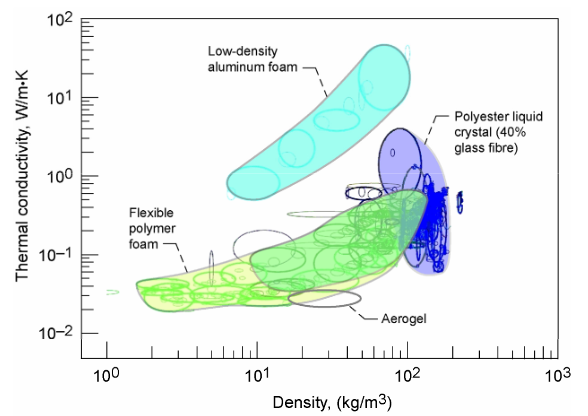
\includegraphics[width=0.75\textwidth]{figure4.png}%

\caption{Отношение термопроводности к удельной плотности для разнообразных инженерных материалов (взято из \cite{ashby2005})}
\label{fig:figure4}
\end{figure}


На \cref{fig:figure5} показан график зависимости теплопроводности (thermal conductivity) от температуропроводности (thermal diffusivity) для различных материалов. Многослойная изоляция имеет тепловую диффузию, сравнимую с семейством металлов, но явную теплопроводность примерно на два порядка ниже, чем у полимерных пен. Для заданной толщины изоляции, следует выбирать систему с наименьшей теплопроводностью, чтобы минимизировать установившийся теплового потока и низкой теплопроводностью, то есть высокой удельной теплоемкостью, чтобы максимизировать время, необходимое для того, чтобы тепловой энергии для достижения криогенной жидкости. Следующее уравнение связывает время достижения устойчивого состояния, \(t\), с толщиной стенки, \(w\), и температуропроводностью, \(a\).
Для заданной толщины стенки желательно минимизировать теплопроводность, чтобы максимизировать время, необходимое для достижения устойчивого состояния, особенно для кратковременных применений. Минимизация отношения \(k/a^{\frac{1}{2}}\), где k - теплопроводность, приводит к максимизации энергии, запасенной в материале для данной дельты температуры и времени. Это максимизирует время, затрачиваемое на то, чтобы тепло могло хранить криогенной жидкости без изменений. 
\[t=\frac{w^2}{2a}\]

\begin{adjustwidth}{3.5em}{3.5em}
{\color{green} Минутка ВИКИПЕДИИ.

Теплопроводность материала (thermal conductivity) --- это мера способности материала проводить тепло через себя. температуропроводность материала (thermal diffusivity), с другой стороны, является тепловой инерцией этого материала.


В физике теплопроводность --- это способность материала проводить тепло. Теплопроводность обозначается символом K. Единицей измерения теплопроводности в СИ является ватт на метр Кельвина (Вт/мК). Теплопроводность данного материала часто зависит от температуры и даже от направления теплопередачи. Согласно второму закону термодинамики, тепло всегда течет от горячей области к холодной. Другими словами, для чистого переноса тепла необходим градиент температуры. Чем выше теплопроводность материала, тем выше скорость передачи тепла через этот материал. 


Температуропроводность (коэффициент температуропроводности) --- физическая величина, характеризующая скорость изменения (выравнивания) температуры вещества в неравновесных тепловых процессах. Численно равна отношению теплопроводности к удельной теплоёмкости при постоянном давлении.  Ее можно понимать как способность материала проводить тепло относительно тепла, аккумулированного в единице объема. Это означает, что чем выше теплопроводность, тем выше температуропроводность.  Температуропроводность газа очень чувствительна к температуре, а также к давлению. Единицей измерения теплопроводности в СИ является м2с-1.
}
\end{adjustwidth}

\begin{figure}[h!]
\centering
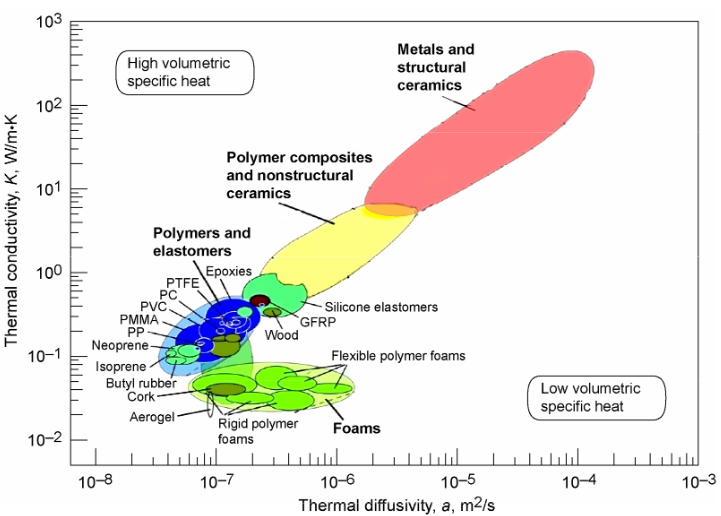
\includegraphics[width=0.75\textwidth]{figure5.png}%
\caption{Отношение теплопроводности от температурапроводности для разнообразных материалов  (взято из \cite{ashby2005}). GFRP -- стеклопластик, PC--- поликарбон, PMMA -- полиметилметакрилат (органическое стекло), PP -- полупропилен, PTFE -- тефлон и PVC -- поливинилхлорид}
\label{fig:figure5}
\end{figure}

На \cref{fig:figure6} показана зависимость теплопроводности от коэффициента теплового расширения для различных материалов. Также на рисунок добавлен примерный режим работы аэрогеля, основанный на данных M.A. Meador (\cite{meador2005}, Исследовательский центр Гленна, Кливленд, штат Огайо, личное сообщение). Этот график полезен для оценки теплового искажения. Значение \(\frac{k}{\alpha}\), где \(\alpha\) -- КТР, может быть использовано в качестве показатель термического искажения. Материалы с большим значением этого показателя демонстрируют небольшое термическое искажение.


Изоляционные материалы по своей функциональности, имея низкие значения теплопроводности, показывают большие тепловые градиенты и, следовательно, высокие тепловые искажения.  Таким образом, материалы с низкой теплопроводностью и, кроме того, обладающие низким КТР, являются желательными. Высокое тепловое искажение может привести к сравнительно большому относительному перемещению, которое может вызвать напряжение в изоляционном материале, превышающее его прочность. прочность материала. Механическое разрушение может привести к ухудшению тепловых свойств изоляционной системы. После выбора класса материалов на основе их тепловых характеристик следует использовать материалы с наименьшим значением \(\alpha\), чтобы минимизировать тепловое искажение и вызванные им напряжения.

Низкая теплопроводность является важным свойством для любой изоляционной системы, особенно для долгосрочного применения. В результате, из \cref{fig:figure6} видно, что жесткие полимерные пенопласты, включая аэрогели, являются жизнеспособной изоляционной системой, поскольку они обеспечивают низкую теплопроводность. Аэрогели в этой группе, по-видимому, имеют более низкий КТР. Как показано на \cref{fig:figure6}, металлические материалы обладают более низким КТР, что приводит к меньшим искажениям; однако их более высокая теплопроводность (и плотность) не позволяет рассматривать их в качестве изоляционных материалов.

\begin{figure}[h!]
\centering
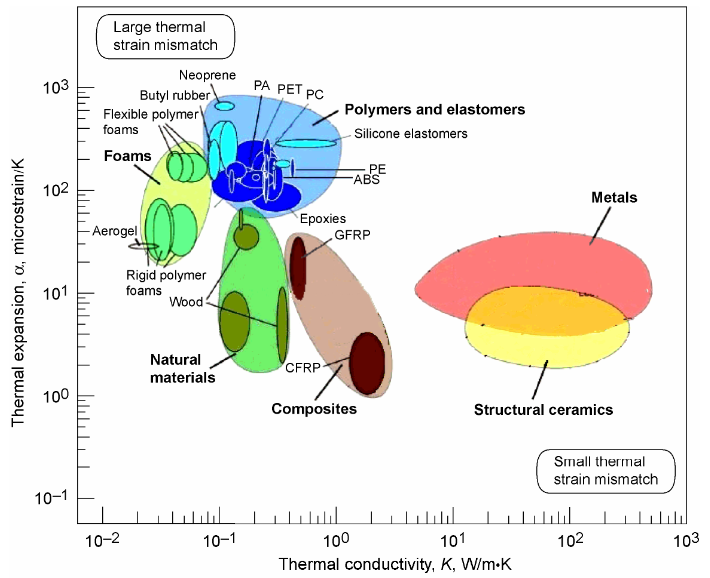
\includegraphics[width=0.75\textwidth]{figure6.png}%
\caption{Отношение КТР от теплопроводности для разнообразных материалов  (взято из \cite{ashby2005}). ABS -- АБС-пластик, GFRP -- стеклопластик, PC--- поликарбон, PMMA -- полиметилметакрилат (органическое стекло), PP -- полупропилен, PTFE -- тефлон и PVC -- поливинилхлорид}
\label{fig:figure6}
\end{figure}

Диапазон значений теплопроводности различных материалов обусловлен уровнем вакуума и разницей температур. Например, системы МСИ обеспечивают очень низкие значения относительной теплопроводности порядка \(10^{-6} \text{Вт/м} \cdot \text{K} (6\times10^{-7} \text{БТу/фут}\cdot \text{час}^{\circ}F)\).
В системах МСИ используется несколько экранов теплового излучения, расположенных перпендикулярно направлению теплового потока. Радиационные экраны представляют собой чередующиеся слои металлической фольги с низкой излучательной способностью (обычно алюминизированный майлар (DuPont)) и тонкая изолирующая прокладка (обычно полиэстер или стекловолоконная бумага), соединенные таким образом, чтобы исключить контакт металла с металлом. Однако существуют строгие требования, которые необходимо учитывать при выборе системы МСИ. Главным требованием к системе МСИ является поддержание уровня вакуума ниже 13 МПа , чтобы система МСИ сохраняла свою эффективность. Теплопередача за счет остаточной газопроводности происходит в условиях пониженного вакуума. Перфорационные отверстия в слоях майлара очень важны для обеспечения отвода остаточных газов при установке вакуумной изоляции и/или системы МСИ. Кроме того, его тепловые свойства сильно анизотропны и чувствительны к механическому сжатию (низкое контактное сопротивление).  Система МСИ была впервые запатентована Матшем (\cite{matsch1961}).

Последние достижения в области МСИ для криогенных резервуаров для хранения включают разработку МСИ с переменной плотностью (МСИПП), где расстояние между слоями варьируется в поперечном сечении МСИ. Радиационная теплопередача обычно преобладает в более теплых внешних слоях стандартной системы МСИ, в то время как теплопроводность играет большую роль в более холодных внутренних слоях. За счет большего расстояния между внутренними слоями уменьшается как масса МСИПП, так и тепловые утечки. Недавно Гастингс и др. (\cite{hastings2004}) провели испытания гибридной системы изоляции из напыляемой пены (SOFI) и МСИПП для орбитального применения. Эта система спроектирована таким образом, чтобы полагаться на SOFI при высоком давлении во время наземного удержания и запуска и на МСИ во время орбиты. 45-слойное одеяло МСИПП варьировалось от 8 слоев/см (20 слоев/дюйм.) в холодной области до 16 слоев/см (41 слой/дюйм.) в теплой области. Испытания показали, что по сравнению со стандартным МСИ с 70 равномерно распределенными слоями уменьшилось выкипание на 41 процент.


Другой предложенной системой изоляции была изоляция микросферами, которая состоит из полых стеклянных сфер различного диаметра и толщины стенок. Она не так чувствительна к условиям вакуума, как МСИ, а также обеспечивает некоторую структурную поддержку с минимальным увеличением низкой теплопроводности при сжимающих нагрузках. Влияние двух промежуточных газов, азота и гелия, при различных давлениях на относительную теплопроводность микросферной изоляции было экспериментально оценено и соотнесено с аналитическими моделями Каннингтоном и Тьеном (\cite{cunnington1978}). Дальнейшие усилия Пармли и Каннингтона (\cite{parmleycunnington1979}) позволили получить данные для проектирования гибкой системы микросферной изоляции из нержавеющей стали в вакуумной оболочке. Современные разработки включают производство автономных эвакуированных изоляционных панелей из микросфер, заключенных в гибкую вакуумную барьерную пленку (Allen et al., \cite{allen2004}). Эти панели обладают теплопроводностью, составляющей примерно половину теплопроводности пенополиуретана.


Другой класс материалов, которые рассматриваются для криоизоляции, -- аэрогель кремнезема. Аэрогели кремнезема -- это твердые вещества с высокой пористостью и очень низкой плотностью, состоящие из взаимосвязанных частиц, которые образуют "открытую" микроструктуру. Теплопроводность аэрогелей кремнезема, как правило, очень низкая, обычно менее \(40\times10^{-3} \text{Вт/м} \cdot K (23 \cdot 10^{-3} \text{БТу/фут} \cdot \text{час}\cdot ^{\circ}F) \), что обусловлено очень низкой теплопроводностью кремнезема, а также размерами пор, которые составляют порядка нанометров. Чрезвычайно низкая теплопроводность делает аэрогели кремнезема очень востребованными для широкого спектра изоляционных применений. Однако те же свойства аэрогелей, которые делают их чрезвычайно хорошими изоляторами -- высокая пористость и низкая плотность -- также делают их по своей природе хрупкими и ломкими. Таким образом, их использование в несущих нагрузку приложениях (таких как криогенные резервуары для хранения LH2 для полетов) является проблематичным. В настоящее время ведутся исследования по улучшению механических свойств аэрогелей без чрезмерного ущерба для их других уникальных свойств. Однако
признано, что любое улучшение механических свойств происходит за счет увеличения плотности массы и, следовательно, увеличения веса и теплопроводности. Один из подходов, использованных Каннингтоном, Ли и Уайтом (1997), заключается в создании композитов волокно/аэрогель путем добавления небольшой объемной доли (менее 5 процентов) коротких волокон кремнезема или карбида кремния. Волокна уменьшают прозрачность для теплового излучения при температурах выше температуры окружающей среды, тем самым увеличивая тепловые характеристики. Волокна также укрепляют аэрогель. Однако этот подход имеет значение только тогда, когда излучение является основным способом передачи тепла, по сравнению с твердофазным и газофазным способами теплопроводности, которые возникают при температурах выше 27 °C (80 °F) и 127 °C (260 °F) соответственно. В Исследовательском центре НАСА имени Гленна также ведутся работы по созданию аэрогелей из сшитого кремнезема, модифицированных эпоксидными смолами для получения механически прочного, но легкого пористого материала (Meador et al., 2005, и Leventis et al., 2003).


\subsection{Возможные материалы и особенности конструкции резервуаров}\label{ch:overview:1:sec4:sub2}

Хранение жидкого водорода в легком резервуаре само по себе представляет значительные трудности. Более низкая плотность водородного топлива приводит к необходимости использования емкости большего объема по сравнению с другими видами топлива. Механические нагрузки на бак определяются (1) разницей между давлением внутри бака и окружающей средой, (2) весом топлива, (3) ускорением транспортного средства, (4) проскальзыванием топлива при маневрах самолета и (5) весом системы бака и его опор. При маневрировании летательного аппарата или при столкновении с воздушной турбулентностью во время полета обязательно возникнет всплеск/бултыхание топлива.

Для поддержания водорода в жидком состоянии необходимо поддерживать постоянное абсолютное давление во внутреннем резервуаре. Давление также будет способствовать перекачке водорода из бака к силовой установки. Холл и Сильверштейн (\cite{hallsilverstein1955}) предположили, что 2 атм (200 кПа, 29 psi) будет достаточно для перекачки топлива в крейсерском режиме для летательного аппарата. Петти (2002) также подтвердил, что внешний бак космического челнока работает в диапазоне давлений 220-230 кПа (32-34 psi), что близко к диапазону, предложенному Холлом и Сильверстайном. Кроме того, с увеличением рабочего давления увеличивается проектный вес бака. Поэтому крайне желательно поддерживать давление в резервуаре как можно более низким, как отметил Рейнольдс (\cite{reynolds1955}). Как правило, газообранзый водород используется в качестве нагнетателя для жидкого водорода.

Два важных критерия для стенки резервуара включают выбор материала и конструкции стенки. Существует множество вариантов, и они обсуждаются в следующих разделах. Обсуждаются преимущества и недостатки различных вариантов, а также даются рекомендации по выбору оптимальной системы.

\subsubsection{Выбор материала стенки резервуара}\label{ch:overview:1:sec4:sub2:subsub1}

Очевидно, что желательно использовать материалы, обладающие высокой прочностью, высокой вязкостью разрушения и высокой жесткостью, а также низкой плотностью и низкой проницаемостью для жидкого и газообразного водорода; однако ни один материал не обеспечивает все эти свойства одновременно.
Следовательно, показатели характеристик материала связаны с этими свойствами. Среди этих параметров прочность и плотность имеют большую значимость для расчета. На \cref{fig:figure7} показана зависимость прочности от массовой плотности для различных инженерных материалов. В данном случае предпочтительными являются материалы, расположенные в левом верхнем углу.
Композитные материалы обладают высокой удельной прочностью по сравнению с металлами и вполне подходят для аэрокосмических применений. В частности, из \cref{fig:figure7} видно, что композиты из полимеров, армированных непрерывным волокном (CFRP, углепластик), обеспечивают самую высокую прочность и при этом являются наиболее легкими. Однако использование композитных материалов, армированных непрерывным волокном, скорее всего, повлечет за собой более высокие первоначальные производственные затраты. Согласно \cref{fig:figure7}, материалами, обладающими достаточной прочностью и приемлемой низкой плотностью, являются КПМ и металлические материалы.
материалы. Керамические материалы также обладают высокой удельной прочностью, но из-за низкой вязкости разрушения они не подходят для использования в качестве материала стенки резервуара.

Потенциальной более дешевой альтернативой композитам, армированным непрерывным волокном, могут быть металлические композиты с дискретным армированием (КДА), в частности, дискретно армированный алюминий (ДАА), описанный Miracle (\cite{miracle2005}). ДАА являются по существу изотропными и могут быть изготовлены с использованием менее дорогостоящих технологий, таких как литье. На \cref{fig:figure8} показан удельный модуль упругости относительно удельной прочности. На этом рисунке желательно использовать материалы, расположенные ближе к правому верхнему углу. Материалы КДА хорошо сопоставляются с композитными материалами на основе полимеров. Дополнительным преимуществом материалов КДА является чрезвычайно низкая (если не пренебрежимо малая) газопроницаемость водорода, обычно связанная с композитными системами на основе полимерных матриц.


\begin{figure}[h!]
\centering
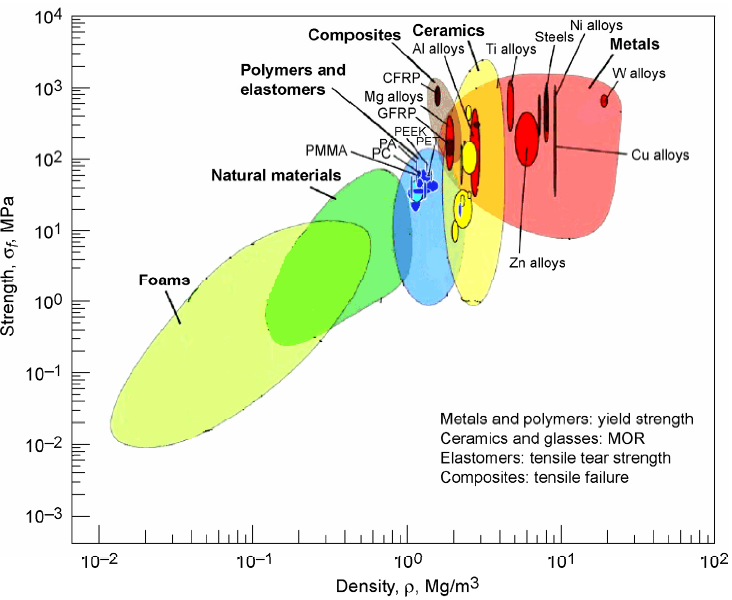
\includegraphics[width=0.75\textwidth]{figure7.png}%
\caption{Отношение прочности к массовой плотности для разнообразных материалов  (взято из \cite{ashby2005}). CFRP -- углепластик, GFRP -- стеклопластик, PA --- полианилин. PC--- поликарбон, PEEK --- полиэфирэфиркетон, PET --- полиэтилен ,PMMA -- полиметилметакрилат (органическое стекло)}
\label{fig:figure7}
\end{figure}

\begin{figure}[h!]
\centering
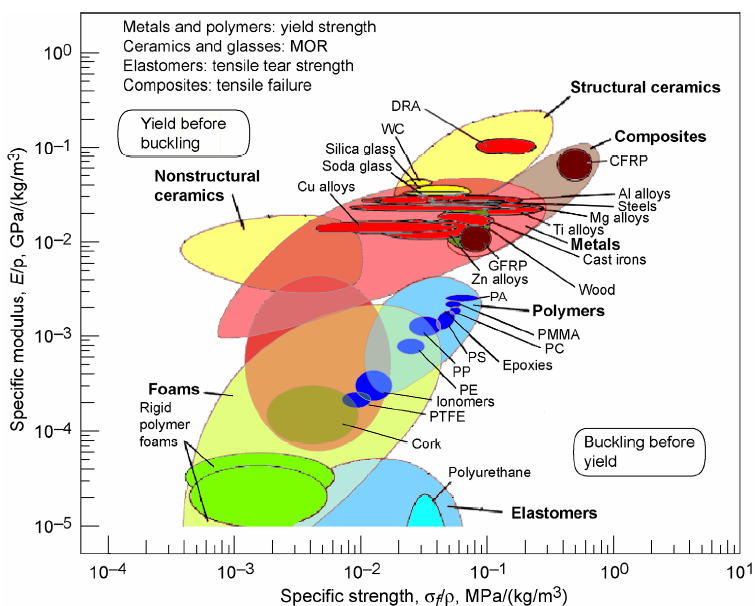
\includegraphics[width=0.75\textwidth]{figure8.png}%
\caption{Отношение удельной модуль упругости от удельной прочности для разнообразных материалов  (взято из \cite{ashby2005}). CFRP -- углепластик, DRA -- дискретно-армированный алюминий, GFRP -- стеклопластик, PA --- полианилин. PC--- поликарбон, PE --- полиэтилен ,PMMA -- полиметилметакрилат (органическое стекло)}
\label{fig:figure8}
\end{figure}

Ключевыми свойствами материала, которые важны для проектирования сосудов высокого давления, но также могут быть применимы к криогенным резервуарам низкого давления, являются <<текучесть до разрушения>>, \(K_{Ic}/\sigma_f\), и <<утечка до разрушения>>, \(K_{Ic}2/\sigma_f\). Они могут быть получены из \cref{fig:figure9}, где \(K_{Ic}\) -- вязкость разрушения, а \(\sigma_f\) -- прочность материала. Использование первого показателя гарантирует, что напряжение, необходимое для распространения критического дефекта, будет больше, чем напряжение, необходимое для деформации материала. Таким образом, сосуд будет стабильно деформироваться таким образом, чтобы его можно было обнаружить. Второй критерий, используемый в основном для больших сосудов, гарантирует, что максимальное давление приведет к стабильному росту трещины, достаточно большой для проникновения как во внутреннюю, так и во внешнюю поверхность, так что утечка может быть обнаружена до катастрофического разрушения. Заметим, что оба показателя могут быть максимизированы, уменьшая предел текучести самой стенки, однако это может не только ограничить способность сосуда выдерживать давление, но и привести к чрезмерно большой толщине стенок и, следовательно, к очень тяжелому резервуару. Толщина стенки резервуара \(t\) определяется следующим уравнением для тонкостенных сферических резервуаров: 

\[t \geq \frac{pR}{2 \sigma_f}\]

где \(p\) -- давление в резервуаре, \(R\) -- радиус резервуара, а \(\sigma_f\) -- прочность материала резервуара, как показано на \cref{fig:figure8}. Чтобы минимизировать массу резервуара и понимая, что масса резервуара прямо пропорциональна толщине стенки резервуара, желательно выбрать такой материал для стенки резервуара, который максимизирует удельную предельную прочность.

\begin{figure}[h!]
\centering
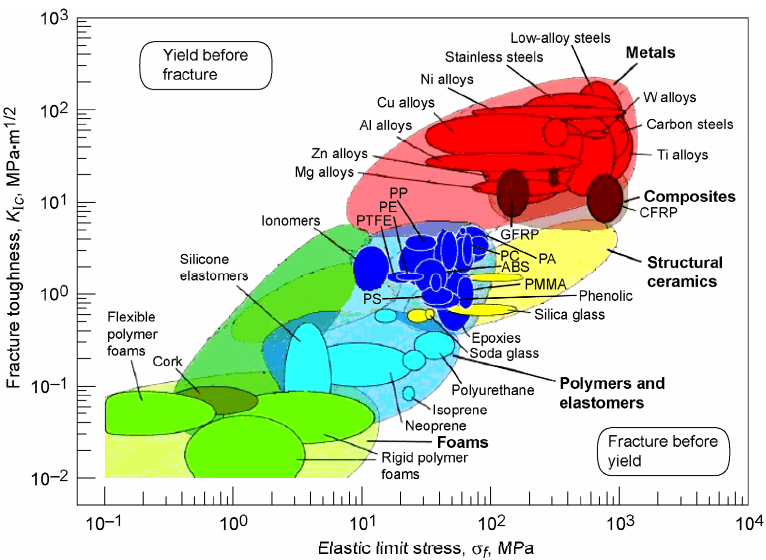
\includegraphics[width=0.75\textwidth]{figure9.png}%
\caption{Отношение вязкости разрушения от прочности для разнообразных материалов  (взято из \cite{ashby2005}). CFRP -- углепластик, DRA -- дискретно-армированный алюминий, GFRP -- стеклопластик, PA --- полианилин. PC--- поликарбон, PE --- полиэтилен, PMMA -- полиметилметакрилат (органическое стекло)}
\label{fig:figure9}
\end{figure}

Рассмотрим следующие параметры материала 
\[ M_1 = \frac{\rho}{\sigma_f} \]
\[ M_2 = \frac{\rho}{K_{Ic}} \]

Первый индекс \(M_1\) основан на требовании, чтобы прочность материала стенки не была превышена, в то время как второй индекс материала \(M_2\) основан на требовании, чтобы вязкость разрушения материала не была превышена. Масса тонкостенного сферического резервуара с радиусом \(R\) и толщиной стенки \(t\) определяющаюся как
\[ m = \left (\pi c \right)^{1/2} M_2 \]

Действующее напряжение в баке от действия внутреннего давления
\[ \sigma = \frac{p R}{2 t}\]

Минимизирую массу резервуара с учетом показанных параметров выше, объеденяя оба параметра, получим
\[ M_1 = \left ( \pi c \right ) ^{1/2} M_2\]
где \(c\) критический размер трещины для данного материала.

На \cref{fig:figure10} показан соответствующий график с двумя линиями связи, соответствующими длинам трещин 5 мм и 5 мкм. Это показывает, что выбор материала может быть ограничен способностью обнаруживать трещины заданного размера. Например, выбор материала будет ограничивается монолитными металлическими сплавами, если можно обнаружить только трещины размером более 5 мм. Однако, как показано на \cref{fig:figure10}, другие материалы, включая керамику и эластомеры, могут быть жизнеспособными материалами, если трещины размером 5 мкм
или больше могут быть обнаружены.

\begin{figure}[h!]
\centering
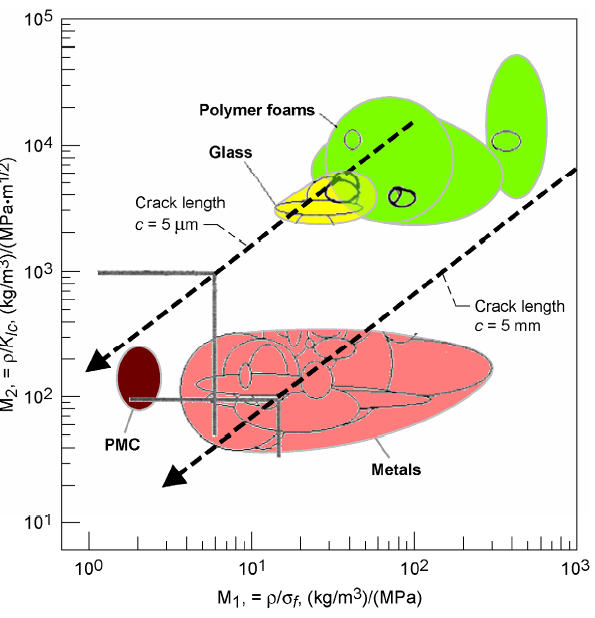
\includegraphics[width=0.75\textwidth]{figure10.png}%
\caption{Два рассматриваемых показателей качества для разнообразных материалов  (взято из \cite{ashby2005}). M1 -- протность/прочность, M2 -- плотность/вязкое разрушение. PMC композит на полимерной матрице}
\label{fig:figure10}
\end{figure}

\begin{figure}[h!]
\centering
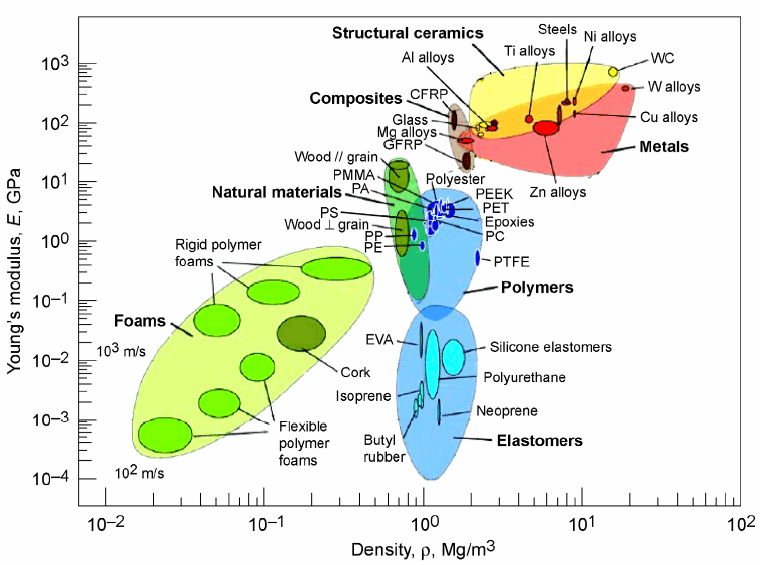
\includegraphics[width=0.75\textwidth]{figure11.png}%
\caption{Отношение вязкости разрушения от прочности для разнообразных материалов  (взято из \cite{ashby2005}). CFRP -- углепластик, DRA -- дискретно-армированный алюминий, GFRP -- стеклопластик, PA --- полианилин. PC--- поликарбон, PE --- полиэтилен, PMMA -- полиметилметакрилат (органическое стекло)}
\label{fig:figure11}
\end{figure}


Отметим, что композитные материалы, в целом, обеспечивают высокую вязкость разрушения наряду с низкой удельной плотностью, что делает их желательными для данного применения. Вязкость разрушения становится проблемой, особенно при криогенных температурах, когда многие материалы становятся чрезмерно хрупкими. Материалы с более высокой вязкостью разрушения желательны, поскольку они обеспечивают более устойчивые к повреждениям системы. Любая трещина, распространяющаяся в системе изоляции, может нарушить тепловые свойства системы изоляции -- что приведет к провалу миссии, поскольку произойдет быстрое выкипание криогенного топлива. На \cref{fig:figure11} представлен модуль Юнга E в зависимости от массовой плотности \(\rho\) для различных используемых материалов. Хотя это и не является основной переменной при проектировании, желательно выбрать жесткий материал, который минимизирует деформацию при нагрузках при сохранении низкой массы. Как и раньше, КПМ и металлические материалы обеспечивают желательную удельную жесткость для данного применения.



Анализируя рисунки \cref{fig:figure7}---\cref{fig:figure11}, можно сказать, что варианты материалов для стенки резервуара включают металлы, КПМ и металломатричные композиты (ММК). Композитные материалы могут также включать многослойную конструкцию, а также материалы, армированные наноразмерными частицами. Как отмечает Эсгар (\cite{esgar1962}), отношение прочности к плотности материала должно быть как можно выше, при этом материал должен иметь минимальные проблемы с изготовлением и не подвержен критическому хрупкому разрушению. Проникновение водорода в структуру резервуара должно быть сведено к минимуму. Металлы, обладающие приемлемыми свойствами от температуры окружающей среды до криогенных температур, включают аустенитные нержавеющие стали, монель и алюминиевые сплавы, как отмечает Рейнольдс (\cite{reynolds1955}). Кроме того, титан и медь обладают приемлемыми свойствами для криогенной эксплуатации, согласно Vance (\cite{vance1964}).

Имеется преимущество в использовании монолитного материала для создания резервуара, как в случаях, упомянутых выше выше. Использование одного материала для стенки резервуара устраняет термически индуцированные внутренние напряжения, вызванные различными КТР , таких как типичные составляющие материала КПМ или MMC. Однако, скорее всего, монолитные металлические резервуары будут не такими легкими, как их аналоги из КПМ или КДА. Металлическая структура подходит для наземных систем, где вес не является столь значительным ограничением, как для аэронавтики или систем космического базирования.

Композитные материалы, в частности КПМ, обладают меньшей плотностью и более высокой прочностью и жесткостью, чем металлы. используемых для криогенных задач. По оценкам, композиты могут обеспечить 25-процентную экономию веса по сравнению с новейшими монолитными алюминиевыми резервуарами в этом применении, как сообщает Sharke (\cite{sharke2004}).
Хотя смолы, используемые в полимерных матричных композитах, имеют склонность к более высокой проницаемости водорода. чем металлы. Брюер (\cite{brewer1991}) отметил, что традиционные композитные структуры с намотанными нитями традиционно не использовались для водородных резервуаров из-за диффузии водорода через промежутки в ив течение длительного времени. Однако разработка композитных баков началась в рамках программы NASP.  Робинсон и др. (\cite{robinson2002}) сообщили, что на основании результатов первоначальных исследований водородная проницаемость не является техническим препятствием для разработки композитного резервуара без вкалыдыша.

Материалы, которые подходят для применения в качестве стенок резервуара, включают монолитные металлы, непрерывно-армированные волокно армированные КПМ, и КДА. Это те классы материалов, которые должны быть дополнительно оценены основываясь на показателях эффективности, рассмотренные выше. Механические свойства, водородная проницаемость, технологичность и стоимость - это некоторые из прочих важных вопросов, которые следует рассмотреть для определения наиболее оптимальной системы материалов для строительства стенки резервуара.

\subsubsection{Особенности конструкции стенки резервуара}\label{ch:overview:1:sec4:sub2:subsub2}

Выбор материала для стенки резервуара -- это лишь один из важных вопросов в процессе проектирования. Геометрия стенки резервуара - еще один важный вопрос. В прошлом использовались различные конфигурации стенок резервуара.  Многие из предыдущих аэрокосмических применений были относительно краткосрочными. В результате одностенная конструкция с ребрами жесткости был распространен. В более поздних экспериментальных проектах использовались двустенные конструкции, включая композитные многослойные конструкции, но с газовой продувкой, а не с вакуумной оболочкой.

Схемы конструкции стенок требуют более глубокого исследования для определения оптимальной, легкой конструкции с соответствующим методом изоляции для удовлетворения потребностей применения в самолете. В \cref{tab:table6} кратко изложены преимущества и недостатки различных методов строительства стенок бака. Изгибающие напряжения в баке возникают в результате всплеска топлива и нагрузок, возникающих на опорных точках. Форма резервуара влияет на его способность выдерживать эти напряжения. Определенные геометрические формы, такие как сфера, могут минимизировать изгибающие напряжения в стенке резервуара. Таким образом, если резервуар должен быть изготовлен в виде цилиндрической конфигурации или более сложной правильной геометрии, то может оказаться полезным выбрать конструкцию стенки, способную выдерживать изгиб.

Две общие категории конструкции стенок резервуара - это одностенные и двустенные конструкции. В связи с необходимостью поддержания низкого теплового потока в течение длительного времени для данного применения используется изолирующая система, как обсуждалось в предыдущем разделе, скорее всего, будет состоять из высоковакуумной основы, что обуславливает использование двустенной конструкции резервуара.

Одностенные конструкции имеют преимущества относительно простой конструкции и низкой стоимости. Однако они могут использоваться только с изоляционной системой на основе пены или аналогичной, и поэтому вряд ли смогут удовлетворить требование низкого теплового потока сквозь стенку для применения в ЛА. Одностенная пенопластовая система вполне подходит для относительно краткосрочного применения, например, для космического челнока "space shuttle".

Двустенная конструкция, напротив, может представлять собой конструкцию типа "сэндвич" с несущей сердцевиной, которая выдерживает различные нагрузки. Кроме того, материал сердцевины может обладать изоляционными свойствами, что ограничивает тепловой поток в бак. В качестве альтернативы, в двустенной конструкции могут использоваться две структурные стенки с минимальным физическим контактом с высоковакуумной изоляционной системой.


\begin{table}
\centering
\small
\caption{Преимущества и недостатки различных конфигураций стенок резервуара для хранения жидкого водорода}
\label{tab:table6}
\begin{tabular}{|l|l|}
\hline
\multicolumn{2}{|c|}{\textbf{Одностенная конструкция}}                                                                                                                                                                                           \\ 
\hline
"+" & \begin{tabular}[c]{@{}l@{}}Простая конструкция\\Не дорогое производство\end{tabular}                                                                                                                                                        \\ 
\hline
"-" & \begin{tabular}[c]{@{}l@{}}Ограниченное количество схем изоляций\\Не оптимальная по весу конструкция\\Не практично при долгосрочном применении\end{tabular}                                                                                 \\ 
\hline
\multicolumn{2}{|c|}{\textbf{Двустенная конструкция}}                                                                                                                                                                                                     \\ 
\hline
"+" & \begin{tabular}[c]{@{}l@{}}Оптимальная по весу конструкция\\Больше схем изоляции\end{tabular}                                                                                                                                               \\ 
\hline
"-" & \begin{tabular}[c]{@{}l@{}}Высокая стоимость\\Сложное производство\end{tabular}                                                                                                                                                             \\ 
\hline
\multicolumn{2}{|c|}{\textbf{Постоянная толщина}}                                                                                                                                                                                                 \\ 
\hline
"+" & \begin{tabular}[c]{@{}l@{}}Простая конструкция\\Не дорогое производство\end{tabular}                                                                                                                                                        \\ 
\hline
"-" & \begin{tabular}[c]{@{}l@{}}Ограниченное количество схем изоляции\\Не оптимальная по весу конструкция\\Не оптимально при долгосрочном использовании\end{tabular}                                                                             \\ 
\hline
\multicolumn{2}{|c|}{\textbf{Переменная толщина (ребра жесткости)}}                                                                                                                                                                               \\ 
\hline
"+" & \begin{tabular}[c]{@{}l@{}}Легковесная конструкция\\Можно оптимизировать под конкретное применение\\Адаптируемые свойства\end{tabular}                                                                                                      \\ 
\hline
"-" & \begin{tabular}[c]{@{}l@{}}Сложное изготовлени\\Высокая стоимость\\Ограниченное количество схем изоляции\\Не оптимально при долгосрочном использовании\end{tabular}                                                                         \\ 
\hline
\multicolumn{2}{|c|}{\textbf{Стенка с наполнителем (сендвич)}}                                                                                                                                                                                    \\ 
\hline
"+" & \begin{tabular}[c]{@{}l@{}}Легковесная конструкция\\Хорошо подходит для нагрузок в плоскости и при изгибе\\Лучшие механическте свойства\\Наполнитель может иметь изоляционные свойства\end{tabular}                                         \\ 
\hline
"-" & \begin{tabular}[c]{@{}l@{}}Проблемы изготовления для больших конструкций (размер)\\Высокая цена\end{tabular}                                                                                                                                \\ 
\hline
\multicolumn{2}{|c|}{\textbf{Неструктурный наполнитель}}                                                                                                                                                                                          \\ 
\hline
"+" & \begin{tabular}[c]{@{}l@{}}Легковесный\\Хорошо подходит к экстремально низким температурам и вакууму\end{tabular}                                                                                                                           \\ 
\hline
"-" & \begin{tabular}[c]{@{}l@{}}Более толстые стенки, больший вес\\Сложность производства и стоимость\\Критически важным является поддержание высокого уровня вакуума,\\поэтому потеря вакуума приводит к катастрофическому отказу\end{tabular}  \\
\hline

\end{tabular}
\end{table}
		% Вводная часть про корабли НАСА
\chapter{Простая постановка задачи}\label{ch:ch1}

\section{Цилиндр с радиальным изменением температуры}\label{sec:ch1/sec1}

Рассмотрим сплошной цилиндр с осью симметрии \(oz\) и радиусом \(b\) и с законом изменения радиальной температуры выраженной \(\theta(r)=T(r)-T_0\), где \(T_0\)~--- начальная температура. Предположим также плоскюу деформацию \(\epsilon_{zz}=\epsilon_{rz}=\epsilon_{\phi z}=0\). Тогда напряженно-деформированное состояние запишется в виде (записываем сразу в цилиндрических координатах и продолжаем работать в них):
\begin{equation}
	\label{eq:ch1:equation1}
\begin{split}
	\epsilon_{rr} &= \frac{1}{E} \big [\sigma_{rr} - \nu \big(\sigma_{\phi\phi} + \sigma_{zz}\big) \big] + \alpha \theta \\
	\epsilon_{\phi\phi} &= \frac{1}{E} \big [\sigma_{\phi\phi} - \nu \big(\sigma_{rr} + \sigma_{zz}\big) \big] + \alpha \theta \\
	\sigma_{zz} &= \nu \big(\sigma_{rr} + \sigma_{\phi\phi}\big) - E\alpha\theta \\
\end{split}
\end{equation}	

Выразим напряжения через деформации, получим
\begin{equation}
	\label{eq:ch1:equation2}
	\begin{split}
		\sigma_{rr} = \frac{E}{(1+\nu)(1-2\nu)} \big[\big(1-\nu \big)\epsilon_{rr} + \nu\epsilon_{\phi\phi} - \big(1+\nu\big )\alpha\theta\big] \\
		\sigma_{\phi\phi} = \frac{E}{(1+\nu)(1-2\nu)} \big[\big(1-\nu \big)\epsilon_{\phi\phi} + \nu\epsilon_{rr} - \big(1+\nu\big )\alpha\theta\big] 
	\end{split}
\end{equation}

Уравнение равновесия для осесимметричной задачи выглядит следующим образом:
\begin{equation}
	\label{eq:ch1:equation3}
		\frac {d\sigma_{rr} }{dr} + \frac {\sigma_{rr}-\sigma_{\phi\phi}}{r}=0
\end{equation}
при этом деформации выраженные через радиальные перемещения \(u\) выглядят так:
\begin{equation}
	\label{eq:ch1:equation4}
	\epsilon_{rr} = \frac{du}{dr} \qquad \epsilon_{\phi\phi} = \frac{u}{r}
\end{equation}

Уравнения~\cref{eq:ch1:equation4} подставим в \cref{eq:ch1:equation2}, что дает следующее:
\begin{equation}
	\label{eq:ch1:equation5}
	\begin{split}
		\sigma_{rr} = \frac{E}{(1+\nu)(1-2\nu)} \big[\big(1-\nu \big)\frac{du}{dr} + \nu\frac{u}{r} - \big(1+\nu\big )\alpha\theta\big] \\
		\sigma_{\phi\phi} = \frac{E}{(1+\nu)(1-2\nu)} \big[\big(1-\nu \big)\frac{u}{r} + \nu\frac{du}{dr} - \big(1+\nu\big )\alpha\theta\big] 
	\end{split}
\end{equation}

Подставляя полученные уравнения \cref{eq:ch1:equation5} в уравнение равновесия \cref{eq:ch1:equation3} и немного упрощая, получим уравнение равновесия в радиальных перемещениях \(u\):
\begin{equation}
	\label{eq:ch1:equation6}
	\frac {d}{dr} \big[\frac{1}{r} \frac{d \big(ur \big)}{dr} \big] = \frac{1+\nu}{1-\nu}\alpha\frac{d\theta}{dr}
\end{equation}

Интегрирование \cref{eq:ch1:equation6} дает следующее уравнение:
\begin{equation}
	\label{eq:ch1:equation7}
	u = \frac{1+\nu}{1-\nu} \frac{\alpha}{r} \int_0^r \theta rdr +C_1r +\frac{C_2}{r}
\end{equation}
где \(C_1\) и \(C_2\) постоянные интегрирования. Поскольку перемещения должны быть конечными в центре (\(r=0\)), отсюда следует, что \(C_2\) должно быть равным нулю. Тогда компоненты перемещения в \cref{eq:ch1:equation4} принимаю вид:
\begin{equation}
	\label{eq:ch1:equation8}
	\begin{split}
		\epsilon_{rr} &= \frac{1+\nu}{1-\nu} \frac{\alpha}{r^2} \int_0^r \theta rdr +C_1 + \frac{1+\nu}{1-\nu} \alpha\theta\\
		\epsilon_{\phi\phi} &= \frac{1+\nu}{1-\nu} \frac{\alpha}{r^2} \int_0^r \theta rdr +C_1
	\end{split}
\end{equation}

и напряжения из уравнения \cref{eq:ch1:equation2} превращяются:

\begin{equation}
	\label{eq:ch1:equation9}
	\begin{split}
		\sigma_{rr} &= -\frac{E}{1-\nu} \frac{\alpha}{r^2} \int_0^r \theta rdr +C_1 \frac{E}{\big(1+\nu\big)\big(1-2\nu\big)}\\
		\sigma_{\phi\phi} &= -\frac{E}{1-\nu} \frac{\alpha}{r^2} \int_0^r \theta rdr -\frac{E \alpha \theta}{1-\nu} +C_1\frac{E}{\big(1+\nu\big)\big(1-2\nu\big)}
	\end{split}
\end{equation}

Определим константуу \(C_1\) используя граничные условия
\begin{equation}
	\label{eq:ch1:equation10}
	\sigma_{rr} = 0 \quad \text{на границе} \quad r=b
\end{equation}
что приводит к следующему
\begin{equation}
	\label{eq:ch1:equation11}
	C_1 = \frac{\alpha \big(1+\nu\big) \big(1-2\nu\big)}{\big(1-\nu\big) b^2} \int_0^b \theta rdr
\end{equation}

После подстановки \cref{eq:ch1:equation7} в \cref{eq:ch1:equation9}, получили:
\begin{equation}
	\label{eq:ch1:equation12}
	\begin{split}
		u &= \frac{1+\nu}{1-\nu} \frac{\alpha}{r} \big[ \int_0^r \theta rdr +\big(1-2\nu\big ) \frac{r^2}{b^2}\int_0^b \theta r dr\big]\\
		\sigma_{rr} &= \frac{E \alpha}{1-\nu}\big[ \frac{1}{b^2}\int_0^b \theta rdr -\frac{1}{r^2}\int_0^r \theta r dr\big]\\
		\sigma_{\phi\phi} &= \frac{E \alpha}{1-\nu}\big[ \frac{1}{b^2}\int_0^b \theta rdr +\frac{1}{r^2}\int_0^r \theta r dr - \theta \big]
	\end{split}
\end{equation}

Напряжения в осевом направлении, \(\sigma_{zz}\), получим из \cref{eq:ch1:equation1}

\begin{equation}
	\label{eq:ch1:equation13}
	\sigma_{zz} = \frac{E \alpha}{1-\nu}\big[ \frac{2\nu}{b^2}\int_0^b \theta rdr  - \theta \big]
\end{equation}	
	
Для тонкостенного цилиндра с радиусами \(a\) и \(b\), определяющие уравнения для перемещений записываются в этих границах --- от \(a\) внутреннего радиуса, до \(r\). Из \cref{eq:ch1:equation7}

\begin{equation}
	\label{eq:ch1:equation14}
	u = \frac{1+\nu}{1-\nu} \frac{\alpha}{r} \int_a^r \theta rdr +C_1r +\frac{C_2}{r}
\end{equation}

Подставляя \(u\) из \cref{eq:ch1:equation4} \cref{eq:ch1:equation2}, радиальные напряжения \(\sigma_{rr}\) находятся следующим образом:

\begin{equation}
	\label{eq:ch1:equation15}
	\sigma_{rr} = E \big [-\frac{\alpha}{\big(1-\nu \big) r^2} \int_a^r \theta rdr + \frac{C_1}{\big (1+\nu\big ) \big(1-2\nu \big)} - \frac{C_2}{\big(1+\nu\big) r^2} \big]
\end{equation}


Применим граничные условия
\begin{equation}
	\label{eq:ch1:equation16}
	\begin{split}
		\sigma_{rr} = 0 \quad \text{на границе} \quad r=a\\
		\sigma_{rr} = 0 \quad \text{на границе} \quad r=b
	\end{split}
\end{equation}

приводит к следующему

\begin{equation*}
	\begin{split}
		C_1 &= \frac{\big(1+\nu \big)\big(1-2\nu \big)}{\big(1-\nu \big)}  \frac{\alpha}{\big(b^2-a^2 \big)} \int_a^b \theta rdr\\
		C_2 &= \frac{\big(1+\nu \big)}{\big(1-\nu \big)}\frac{\alpha a^2}{\big(b^2-a^2 \big)}\int_a^b \theta rdr
	\end{split}
\end{equation*}

Подставим \(C_1\) и \(C_2\) в \cref{eq:ch1:equation14}, радиальные перемещения и напряжения получаются следующими:

\begin{equation}
	\label{eq:ch1:equation17}
	\begin{split}
		u &= \frac{1+\nu}{1-\nu} \frac{\alpha}{r} \big[ \frac{\big( 1-2\nu \big) r^2 +a^2}{b^2-a^2} \int_a^b \theta rdr + \int_a^r \theta r dr\big]\\
		\sigma_{rr} &= \frac{E \alpha}{1-\nu}\big[ \frac{1}{b^2-a^2} \big(1-\frac{a^2}{r^2} \big)\int_a^b \theta rdr -\frac{1}{r^2}\int_a^r \theta r dr\big]\\
		\sigma_{\phi\phi} &= \frac{E \alpha}{1-\nu}\big[ \frac{1}{b^2-a^2}\big(1+\frac{a^2}{r^2} \big)\int_a^b \theta rdr +\frac{1}{r^2}\int_a^r \theta r dr - \theta \big]
	\end{split}
\end{equation}	
	
Осевые напряжения из \cref{eq:ch1:equation1}	получаются следующими:

\begin{equation}
	\label{eq:ch1:equation18}
	\sigma_{zz} = \frac{E \alpha}{1-\nu}\big[ \frac{2\nu}{b^2-a^2}\int_a^b \theta rdr  - \theta \big]	
\end{equation}

и осевая сила \(F_z\) в этом случае, \(\epsilon_{zz}=0\)

\begin{equation}
	\label{eq:ch1:equation19}
	F_z = \int_a^b 2 \pi r \sigma_{zz} dr
\end{equation}


Если положить внутреннюю температуру в цилиндре \(T_a\), а внешнюю \(T_b\), то распределение температуры можно записать в виде:

\begin{equation}
	\label{eq:ch1:equation20}
	{\color{red}T=\frac{T_a - T_b}{\ln{\frac{b}{a}}} \big(\ln{\frac{b}{r}} \big) + T_b}
\end{equation}

\[T_a - T_b = T_d\]
{\color{red}TODO: объяснить откуда это пришло?}

Подставляя температурное распределение в напряжения для полого цилиндра с фиксированными гранями \cref{eq:ch1:equation17}, получаем:

\begin{equation}
	\label{eq:ch1:equation21}
	\begin{split}
		\sigma_{rr} &= \frac{E \alpha T_d}{2 \big (1 -\nu \big) \ln{\frac{b}{a}}}\big[ \ln{\frac{b}{r}} + \frac{a^2}{b^2-a^2} \big(1-\frac{b^2}{r^2} \big) \ln{\frac{b}{a}}\big]\\
		\sigma_{\phi\phi} &= \frac{E \alpha T_d}{2 \big (1-\nu \big ) \ln{\frac{b}{a}} }\big[1 - \ln{\frac{b}{r}} - \frac{a^2}{b^2-a^2}\big(1+\frac{b^2}{r^2} \big)\ln{\frac{b}{a}} \big] \\
		\sigma_{zz} &= \frac{\nu E \alpha T_d}{2 \big (1-\nu \big) \ln{\frac{b}{a}}} \big [1-\frac{2 a^2}{b^2 - a^2}\ln{\frac{b}{a}}-\frac{2}{\nu} \ln{\frac{b}{r}} \big] - E \alpha \big(T_b - T_0 \big)
	\end{split}
\end{equation}

Теперь рассмотрим случай обобщенного условия деформации в плоскости для полого толстого цилиндра. Из уравнения ({\color{red}Сослаться на 1.19}) следует, что осевая нагрузка равна нулю

\begin{equation}
	\label{eq:ch1:equation22}
	F_z = \int_a^b 2 \pi r \sigma_{rr} dr = 0
\end{equation}

Если переписать осевую деформацию цилинда \(\epsilon_{zz}\) с нагревом в полярных координатах, то получим

\begin{equation}
	\label{eq:ch1:equation23}
	\sigma_{zz} = r \big (\sigma_{rr}+\sigma_{\phi\phi} \big) + E \alpha (\bar{\theta} - \theta)
\end{equation}

где \(\theta = T - T_0\) и

\begin{equation}
	\label{eq:ch1:equation24}
	\bar{\theta} = \frac{1}{A} \int_A dA = \frac{2 \pi}{\pi \big (b^2 - a^2 \big)} \int_a^b \theta rdr = \frac{2}{b^2-a^2} \int_a^b \theta rdr
\end{equation}


Подставляя компоненты напряжения из \cref{eq:ch1:equation17} в \cref{eq:ch1:equation23} получаем:

\begin{equation}
	\label{eq:ch1:equation25}
	\sigma_{zz} = \frac{E \alpha}{1 - \nu} \big ( \bar{\theta} - \theta \big )
\end{equation}

По-другому, сложив компоненты напряжений (радиальные и тангенсальные) из \cref{eq:ch1:equation17}:

\begin{equation}
	\label{eq:ch1:equation26}
	\sigma_{rr} + \sigma_{\phi\phi} = \frac{E \alpha}{1-\nu} \big [\frac{2}{b^2 - a^2} \int_a^b \theta rdr - \theta \big] = \frac{E \alpha}{1 - \nu} \big ( \bar{\theta} - \theta \big )
\end{equation}

Для этого особого случая
\begin{equation}
	\label{eq:ch1:equation27}
	\sigma_{rr} + \sigma_{\phi\phi} = \sigma_{zz}
\end{equation}

Когда толстостенный цилиндр также подвергается внутреннему и внешнему давлению, \(p_a\) и \(p_b\), соответственно, полное напряжение в цилиндре становится суммой тепловых и механических напряжений. Механические напряжения получаются из тех же управляющих уравнений, за исключением того, что член \(T\) исчезает. Таким образом, последовательное решение этих уравнений для радиального перемещения \(u\) дается уравнением \cref{eq:ch1:equation7} за исключением члена, включающего интеграл от
температуры, который исчезает, а радиальное перемещение становится равным:

\begin{equation}
	\label{eq:ch1:equation28}
	u = C_1 r + \frac{C_2}{r}
\end{equation}

Подставляя это перемещение в \cref{eq:ch1:equation4}, а потом в \cref{eq:ch1:equation2} при следующих граничных условиях

\begin{equation}
	\label{eq:ch1:equation29}
	\begin{split}
		\sigma_{rr} = -p_a \quad \text{на границе} \quad r=a \\
		\sigma_{rr} = -p_b \quad \text{на границе} \quad r=b
	\end{split}
\end{equation}

даёт уравнения радиальных и тангенсальных напряжений для механического нагружения:

\begin{equation}
	\label{eq:ch1:equation30}
	\begin{split}
		\sigma_{rr} = \frac{p_a a^2}{b^2 - a^2} \big (1-\frac{b^2}{r^2} \big )- \frac{p_b b^2}{b^2-a^2} \big (1 - \frac{a^2}{r^2} \big )\\
		\sigma_{\phi\phi} = \frac{p_a a^2}{b^2 - a^2} \big (1+\frac{b^2}{r^2} \big )- \frac{p_b b^2}{b^2-a^2} \big (1 + \frac{a^2}{r^2} \big )
	\end{split}
\end{equation}

Как вывод, когда толстый цилиндр подвергается как тепловым, так и механическим напряжения, результирующие напряжения являются суммой уравнений \cref{eq:ch1:equation21} и \cref{eq:ch1:equation30}.

\section{Неравномерный нагрев цилиндра}
\label{sec:ch1/sec2}
Надеюсь до этого не дойдет. Тут беда. 
Если дойдет, то посмотреть на метод косплексных переменных 

\chapter{Функционально-градиентные материалы}\label{ch:ch2}

Функционально-градиентные материалы (ФГМ) --- это новые передовые жаропрочные материалы, используемые в современных технологиях. Помимо превосходных тепловых свойств и способности выдерживать сверхвысокие термические нагрузки, они обладают коррозионной и
устойчивы к эрозии и обладают высокой прочностью на излом.


Исторически метод создания ФГМ состоит в том, чтобы смешать керамику и металл таким образом, чтобы свойства материала непрерывно изменялись от одного составляющего материала к другому. Фактически, коэффициенты определяющих уравнений для распределения температуры и напряжения зависят от координат, поскольку свойства материала являются функциями положения.

Будем рассматривать степенное изменения свойств материала.

\section{Толстый цилиндр из функционально-градиентного материала} \label{ch:ch2/sec1}

Рассмотрим толстый полый цилиндр внутреннего радиуса \(a\) и внешнего радиуса \(b\) изготовленный из ФГМ. Материал цилиндра имеет градацию по направлению \(r\), поэтому свойства материала являются функциями \(r\). Пусть \(u\) и \(v\) --- компоненты перемещения в радиальном и окружном направлениях, соответственно. Тогда соотношения между деформацией и перемещением имеют вид:

\begin{equation}
	\label{eq:ch2:equation1}
	\begin{split}
		\epsilon_{rr} & = u_{,r}\\
		\epsilon_{\phi\phi} &= \frac{u_{,\phi}}{r} + \frac{u}{r}\\
		\epsilon_{r \phi} &= \frac{1}{2} \big(\frac{u_{,\phi}}{r} - \frac{v}{r} \big)
	\end{split}
\end{equation}
где значок \((,)\) обозначает частную производную. Тогда напряженно-деформированное состояние для плоской деформации запишется в виде:

\begin{equation}
	\label{eq:ch2:equation2}
	\begin{split}
		\sigma_{rr} &= \big(\lambda + 2 \mu \big) \epsilon_{rr} + \lambda \epsilon_{\phi\phi} - \big(3 \lambda +2 \mu \big) \alpha \theta (r, \phi)\\
		\sigma_{\phi\phi} &= \big(\lambda + 2 \mu \big) \epsilon_{\phi \phi} + \lambda \epsilon_{rr} - \big(3 \lambda +2 \mu \big) \alpha \theta (r, \phi)\\
		\sigma_{r \phi} &= 2\mu \epsilon_{r \phi}
	\end{split}
\end{equation}

где \(\sigma_{ij}\) и \(\epsilon_{ij}\) (\(i,j = r,\phi)\) --- тензоры напряжений и деформаций, \(\theta (r, \phi) \) --- распределение температуры, определяемое уравнением теплопроводности, где \(\alpha \) --- коэффициент линейного теплового расширения, а \( \lambda \) и \(\mu \) --- коэффициенты Ламэ.

Уравнения равновесия в радиальном и окружном направлениях, без сосредоточенных сил и сил инерции, имеют вид


\begin{equation}
	\label{eq:ch2:equation3}
	\begin{split}
		\sigma_{rr,r} &+ \frac{1}{r} \sigma_{r \phi, \phi} + \frac{1}{r} \big ( \sigma_{rr} - \sigma_{\phi\phi}\big ) = 0 \\
		\sigma_{r \phi, r} &+ \frac{1}{r} \sigma_{\phi \phi, \phi} + \frac{2}{r} \sigma_{r \phi} = 0
	\end{split}
\end{equation}


Для получения уравнений равновесия в перемещениях
для ФГМ-цилиндра, закон распределения внутренних свойств материала должен быть известен заранее. Поскольку предполагается, что материал цилиндра меняется в \(r\) --- радиальном направлении --- модуль упругости и коэффициент теплового расширения предполагается описывать степенными законами как

\begin{equation}
	\label{eq:ch2:equation4}
	\begin{split}
		E(r) &= E_0 \big ( \frac{r}{l} \big) ^ {m_1} \\
		\alpha (r) &= \alpha_0 \big ( \frac{r}{l} \big) ^{ m_2}
	\end{split}
\end{equation}

где \(E_0\) и \(\alpha_0 \) --- постоянные материала, а \(m_1\) и \(m_2\) --- степенные показатели распределения свойств, \(l\) --- характерная длина. Здесь и далее положим,
что коэффициент Пуассона постоянен.

Подставляя \cref{eq:ch2:equation1} в \cref{eq:ch2:equation4}, уравнения Навье в перемещения записываются в следующем виде.
\begin{adjustwidth}{3.5em}{3.5em} В общем случае напряжения можно выразить через деформации, а затем и перемещения. Если, после взятия частной производной, подставить это в уравнения равновесия, то получатся следующие уравнения, которые называется уравнениеми Навье. В ПДСК это выглядит следующим образом:

\begin{equation*}
\begin{split}
	&\sigma_{ij,j} + X_i = \rho \ddot{u_i} \quad \text{уравнение равновесия} \\
	&\sigma_{ij} = \mu \big (u_{i,j} + u_{j,i} \big ) + \big [ \lambda u_{k,k} - \alpha \big (3 \lambda +2\mu \big ) \big (T-T_0 \big ) \big ] \delta_{ij}\\
	&\mu u_{i,kk} + \big ( \lambda + \mu \big ) u_{k,ki} - \big ( 3 \lambda + 2\mu \big ) \alpha T_{,i} +X_i = \rho \ddot{u_i} \quad \text{уравнение Навье}
\end{split}
\end{equation*}
\end{adjustwidth}


{\color{red} ВОТ ТУТ НУЖНО БЫ ЕЩЕ РАЗИК ПРОВЕИТЬ :

\begin{equation}
	\label{eq:ch2:equation5}
	\begin{split}
		u_{,rr} &+ \big ( m_1+1\big ) \frac{1}{r} u_{,r} + \big ( \frac{\nu m_1}{1-\nu} -1 \big ) \frac{1}{r^2} u + \big ( \frac{1-2\nu}{2-2\nu} \big) \frac{1}{r^2} u_{\phi \phi} + \big ( \frac{1}{2-2\nu}\big ) \frac{1}{r} v_{,r \phi} \\
		&+ \big [ \frac{\big ( 4+2 m_1\big ) \nu -3 }{2-2\nu} \big ] \frac{1}{r^2} v_{, \phi} = \frac{\big ( 1+\nu\big ) \alpha_0 }{\big (1-\nu \big ) l^{m_2}} \Big [ \big (m_1 + m_2 \big ) r^{m_2 -1} \theta + r^{m_2} \theta_{,r}\Big] \\
		%
		v_{,rr} &+ \big (m_1 +1 \big ) \frac{1}{r} v_{,r} - \big (m_1 + 1 \big ) \frac{1}{r^2} v + \big ( \frac{2-2\nu }{1-2\nu } \big ) \frac{1}{r^2} v_{,\phi \phi} + \big ( \frac{1}{1-2\nu} \big ) \frac{1}{r} u_{,r \phi} \\
		&+ \big ( \frac{3-4\nu}{1-2\nu} + m_1\big ) \frac{1}{r^2} u_{, \phi} = \big (\frac{2+2\nu}{1-2\nu} \big ) \big (\frac{\alpha_0 r^{m_2 -1}}{l^{m_2}} \big ) \theta_{,\phi}
	\end{split}
\end{equation}
}


Чтобы получить компоненты перемещения \(u\) и \(v\), распределение температуры должно быть известно. Используя груничные условия ({\color{red} описать ГУ}), закон распределения температруры запишется в виде:

\begin{equation}
	\label{eq:ch2:equation6}
	\theta(r, \phi) = \sum_{n=-\infty}^{+\infty} \big (A_{n1} r^{\beta_{n1}} + A_{n2} r^{\beta_{n2}} \big ) e^{in \phi}
\end{equation}

где \(\beta_{n1}\) и \(\beta_{n2}\) и константы интегрирования \(A_{n1}\) и \(A_{n2}\) определены ранее {\color{red} вот раньше из ГУ} 

При заданном температурном распределении (поле), уравнение Навье может быть разрешено в перемещениях \(u(r, \phi) \) и \(v(r, \phi) \). Компоненты перемещений можно разложить в ряд Фурье как:
\begin{equation}
\label{eq:ch2:equation7}
\begin{split}
	u(r, \phi) &= \sum_{n=-\infty}^{\infty} u_n(r) e^{in\phi}\\
	v(r, \phi) &= \sum_{n=-\infty}^{\infty} v_n(r) e^{in\phi}
\end{split}
\end{equation}
где \(u_n(r)\) и \(v_n(r)\) коэффициенты в разложении Фурье значений \(u(r, \phi)\) и \(v(r, \phi)\) соответсвенно, которые определяются как:

\begin{equation}
\label{eq:ch2:equation8}
\begin{split}
	u_n(r) &= \frac{1}{2\pi} \sum_{-\pi}^{\pi} u(r, \phi) e^{-in\phi} d\phi\\
	v_n(r) &= \frac{1}{2\pi} \sum_{-\pi}^{\pi} v(r, \phi) e^{-in\phi} d\phi
\end{split}
\end{equation}

Подставляя уравнения \cref{eq:ch2:equation6} и \cref{eq:ch2:equation7} в \cref{eq:ch2:equation5}, получим

\begin{equation}
\label{eq:ch2:equation9}
\begin{split}
	&u_n^{\prime\prime} + \big ( m_1 + 1 \big ) \frac{1}{r} u_n^{\prime} + \big [ \frac{\nu m_1}{1-\nu} -1 - \frac{\big ( 1 - 2\nu \big )n^2}{2-2\nu} \big ] \frac{1}{r^2}u_n + \big(\frac{in}{2-2\nu} \big)\frac{1}{r}v_n^{\prime}\\
&+in \big [ \frac{ \big (4+2\nu \big )\nu -3}{2-2\nu}\big ]\frac{1}{r^2}v_n = \frac{\big (1+\nu \big ) \alpha_0}{\big (1-\nu \big )l^{m2}} \big [ \big (m_1 + m_2 +\beta_{n1} \big )A_{n1} r^{\beta_{n1}+m_2-1} \\
&+ \big(m_1 +m_2 + \beta_{n2} \big ) A_{n2} r^{\beta_{n1}+m2-1} \big ]
\end{split}
\end{equation}

\begin{equation}
\label{eq:ch2:equation10}
\begin{split}
	&v_n^{\prime\prime} + \big ( m_1 + 1 \big ) \frac{1}{r} v_n^{\prime} - \big [ m_1 + 1 + \frac{\big (2-2\nu \big )n^2}{1-2\nu} \big ] \frac{1}{r^2}v_n + \big(\frac{in}{1-2\nu} \big)\frac{1}{r}u_n^{\prime}\\
&+ in \big (\frac{3-4\nu}{1-2\nu} + m_1 \big ) \frac{1}{r^2} u_n = \frac{in \big (2+2\nu \big)}{\big (1-2\nu \big) l^{m_2}} \alpha_0 \big [ A_{n1} r^{\beta_{n1}+m_2-1} + A_{n2} r^{\beta_{n_2}+m_2 -1}\big ]
\end{split}
\end{equation}

Уравнения \cref{eq:ch2:equation9} и \cref{eq:ch2:equation10} образуют систему обыкновенных дифференциальных уравнений (СОДУ) с общим и частным решением. Решение в общем виде предполагается найти в виде:

\begin{equation}
\label{eq:ch2:equation11}
\begin{split}
	u_n^g(r) &= Br^{\eta} \quad \text{g --- general --- общее решение}\\
	v_n^g(r) &= Cr^{\eta}
\end{split}
\end{equation}

Подставляя \cref{eq:ch2:equation11} и \cref{eq:ch2:equation9} в \cref{eq:ch2:equation10}, получим:

\begin{equation}
\label{eq:ch2:equation12}
\begin{split}
	&\big [ \eta \big (\eta-1 \big) + \big (m_1 +1 \big) \eta + \frac{\nu m_1}{1-\nu} - 1 -\frac{ \big (1-2\nu \big)n^2}{2-2\nu} \big ] B \\
&+ i \big [\frac{\eta}{2-2\nu} + \frac{\big (4+2m_1 \big ) \nu -3 }{2-2\nu}  \big ] n C=0\\
&i \big [\frac{\eta}{1-2\nu} + \frac{3-4\nu}{1-2\nu} + m_1 \big ]nB+\big [ \eta \big ( \eta-1\big ) + \big (m_1 +1 \big ) \\
&- m_1 -1 \frac{\big (2-2\nu \big ) n^2}{1-2\nu} \big ] C=0
\end{split}
\end{equation}

Для получения нетривиального решения \( (B, C) \) уравнения \cref{eq:ch2:equation12}, \( \eta \) должно удовлетворять следующему уравнению:

\begin{equation}
\label{eq:ch2:equation13}
\begin{split}
	& \left [\eta  \left (\eta -1 \right )+  \left ( m_1 +1 \right ) \eta + \frac{\nu m_1}{1-\nu} -1 - \frac{ \left (1 - 2\nu  \right  ) n^2}{2-2\nu} \right ]  \left [ \eta  \left (\eta -1 \right ) \right. \\
	&+ \left. \left  ( m_1 + 1 \right ) \eta - m_1 - 1 - \frac{ \left ( 2-2\nu  \right ) n^2}{1-2\nu}  \right. ] +n^2 \left [ \frac{\eta}{2-2\nu}  \right. \\
	&+  \left. \frac{  \left ( 4+2 m_1 \right ) \nu -3}{2-2\nu}  \right ] \left  [ \frac{\eta}{1-2\nu} + \frac{3-4\nu}{1-2\nu} +m_1 \right ] = 0
\end{split}
\end{equation}

Уравнение \cref{eq:ch2:equation13} имеет четыре (4) корня --- от \( \eta_{n1} \) до \( \eta_{n4} \). Таким образом, общее решение уравнений \cref{eq:ch2:equation9} и \cref{eq:ch2:equation10} принимает вид:

\begin{equation}
\label{eq:ch2:equation14}
\begin{split}
	u_n^g(r) &= \sum_{j=1}^4 B_{n_j} r^{\eta_{n_j}}\\
	v_n^g(r) &= \sum_{j=1}^4 N_{n_j} B_{n_j} r^{\eta_{n_j}}
\end{split}
\end{equation}
где \( N_{n_j} = C_{n_j} / B_{n_j}\) и получено из первого уравнения \cref{eq:ch2:equation12} как

\begin{equation}
\label{eq:ch2:equation15}
	N_{n_j} = \frac{i \left [ \eta_j \left (\eta_j -1 \right ) + \left ( m_1 +1 \right ) n_j +\frac{\nu m_1}{1-\nu} -1 - \frac{\left (1-2\nu \right ) n^2}{2-2\nu} \right ]}{n \left [ \frac{n_j}{2-2\nu} + \frac{\left (4+2m_1 \right )\nu -3}{2-2\nu} \right ]}
\end{equation}

Для изотропного материала \((m_1=0) \) и для \(n=1\), уравнение \cref{eq:ch2:equation13} имеет несколько корней, рассмотрим решение в виде \( \ln{(r/r_0)},  r_0 > 0\), для \(u_n(r), v_n(r) \).

Поиск частного решения \(u_n^p(r), v_n^p(r) \), будем делать в виде:

\begin{equation}
\label{eq:ch2:equation16}
\begin{split}
	u_n^p(r) &= D_{n_1} r^{\beta_{n_1} + m_1 + 1} + D_{n_2} r^{\beta_{n_2} +m_2 + 1} \quad \text{p --- particular --- частное}\\
	v_n^p(r) &= D_{n_3} r^{\beta_{n_1} + m_2 + 1} + D_{n_2} r^{\beta_{n_4} +m_2 + 1}
\end{split}
\end{equation}

Подставляя уравнение \cref{eq:ch2:equation16} в \cref{eq:ch2:equation9} и \cref{eq:ch2:equation10}, получаем:

\begin{equation}
\label{eq:ch2:equation17}
\begin{split}
	&d_1 D_{n_1} r^{\beta_{n_1}+m_2-1} + d_2 D_{n_2} r^{\beta_{n_2}+m_2-1} + d_3 D_{n_3} r^{\beta_{n_1}+m_2-1} \\
	&+d_4 D_{n_4} r^{\beta_{n_2}+m_2-1} = d_5  r^{\beta_{n_1}+m_2-1} + d_6  r^{\beta_{n_2}+m_2-1}
\end{split}
\end{equation}

\begin{equation}
\label{eq:ch2:equation18}
\begin{split}
	&d_7 D_{n_3} r^{\beta_{n_1}+m_2-1} + d_8 D_{n4} r^{\beta_{n_2}+m_2-1} + d_93 D_{n_1} r^{\beta_{n_1}+m_2-1} \\
	&+d_{10} D_{n_2} r^{\beta_{n_2}+m_2-1} = d_{11} r^{\beta_{n_1}+m_2-1} + d_{12}  r^{\beta_{n_2}+m_2-1}
\end{split}
\end{equation}

где константы от \(d_1\) до \(d_{12}\) определяются по следующим формулам:

\begin{equation*}
\begin{split}
	d_1 &= \big (\beta_{n_1}+m_2-1 \big ) \big (\beta_{n_1}+m_2\big )+ \big (m_1+1 \big ) \big (\beta_{n_1}+m_2+1 \big )+ \frac{\nu m_1}{1-\nu}\\
	& - 1 - \frac{\big (1-2\nu \big )n^2}{2-2\nu}\\
	d_2 & = \big (\beta_{n_2}+m_2-1 \big ) \big (\beta_{n_2}+m_2\big )+ \big (m_1+1 \big ) \big (\beta_{n_2}+m_2+1 \big )+ \frac{\nu m_1}{1-\nu}\\
	& - 1 - \frac{\big (1-2\nu \big )n^2}{2-2\nu}\\
	d_3 &= in \big ( \frac{\beta_{n_1}+m_2-1}{2-2\nu} + \frac{\big (4+2m_1 \big )\nu -3}{2-2\nu}  \big) \\
	d_4 &= in \big ( \frac{\beta_{n_2}+m_2-1}{2-2\nu} + \frac{\big (4+2m_1 \big )\nu -3}{2-2\nu}  \big) \\
	d_5 & = \frac{\big (1+\nu \big )\big (m_1+m_2+\beta_{n_1} \big ) \alpha_0 A_{n_1}}{\big ( 1-\nu \big )l^{m_2}} \\
	d_6 & = \frac{\big (1+\nu \big )\big (m_1+m_2+\beta_{n_2} \big ) \alpha_0 A_{n_2}}{\big ( 1-\nu \big )l^{m_2}} \\
	d_7 & =  \big (\beta_{n_1}+m_2-1 \big ) \big (\beta_{n_1}+m_2\big )+ \big (m_1+1 \big ) \big (\beta_{n_1}+m_2+1 \big ) -m_1 \\
		& - 1 - \frac{\big (2-2\nu \big )n^2}{1-2\nu}\\
	d_8 & =  \big (\beta_{n_2}+m_2-1 \big ) \big (\beta_{n_2}+m_2\big )+ \big (m_1+1 \big ) \big (\beta_{n_2}+m_2+1 \big ) -m_1 \\
		& - 1 - \frac{\big (2-2\nu \big )n^2}{1-2\nu}\\
	d_9 &= in \big ( \frac{\beta_{n_1}+m_2-1}{1-2\nu} + \frac{3-4 \nu}{1-2\nu} +m_1  \big) \\
	d_{10} &= in \big ( \frac{\beta_{n_2}+m_2-1}{1-2\nu} + \frac{3-4 \nu}{1-2\nu} +m_1  \big) \\
	d_{11} &= \frac{in \big(2+2\nu \big ) \alpha_0 A_{n_1}}{\big ( 1-2\nu \big ) l^{m_2}}\\
	d_{12} &= \frac{in \big(2+2\nu \big ) \alpha_0 A_{n_2}}{\big ( 1-2\nu \big ) l^{m_2}}
\end{split}
\end{equation*}

Приравнивая коэффициенты при одинаковых степенях
\begin{equation}
\label{eq:ch2:equation19}
\begin{split}
	d_1 D_{n_1} +d_3 D_{n_3} &= d_5\\
	d_{9} D_{n_1} +d_7 D_{n_3} &= d_{11}
\end{split}
\end{equation}
\begin{equation}
\label{eq:ch2:equation20}
\begin{split}
	d_2 D_{n_2} +d_4 D_{n_4} &= d_6\\
	d_{10} D_{n_2} +d_8 D_{n_4} &= d_{12}
\end{split}
\end{equation}

Уравнения \cref{eq:ch2:equation19} и \cref{eq:ch2:equation20} образуют систему линейных алгебраических уравнений (СЛАУ), где решение можно найти методом Крамера, например:

\begin{equation}
\label{eq:ch2:equation21}
\begin{split}
	D_{n_1} & = \frac{d_5 d_7 - d_3 d_{11} }{d_1 d_7 - d_3 d_{9}} \quad  D_{n_2}  = \frac{d_6 d_8 - d_4 d_{12} }{d_2 d_8 - d_4 d_{10}}\\
	D_{n_3} & = \frac{d_1 d_{11} - d_5 d_{9} }{d_1 d_7 - d_3 d_{9}} \quad  D_{n_4}  = \frac{d_2 d_{12} - d_6 d_{10} }{d_2 d_8 - d_4 d_{10}}
\end{split}
\end{equation}

обеспечивая положительными знаменатели, т.е. \( d_1 d_7 - d_3 d_{9} \ne 0\) и \( d_2 d_8 - d_4 d_{10} \ne 0\). Полное решение для  \(u_n(r), v_n(r) \) определяется как сумма общего и частного решения, запишется в виде:

\begin{equation}
\label{eq:ch2:equation22}
\begin{split}
	u_n(r) & =u_n^g(r)+u_n^p(r)\\
	v_n(r) &= v_n^g(r)+v_n^p(r)
\end{split}
\end{equation}

Отсюда

\begin{equation}
\label{eq:ch2:equation23}
\begin{split}
	u_n(r) & =\sum_{j=1}^4 B_{n_j} r^{\eta_{n_j}} + D_{n_1} r^{\beta_{n_1} +m_2 +1} +D_{n_2} r^{\beta_{n_2} +m_2 +1} \\
	v_n(r) &= \sum_{j=1}^4 N_{n_j} B_{n_j} r^{\eta_{n_j}} + D_{n_3} r^{\beta_{n_1} +m_2 +1} +D_{n_4} r^{\beta_{n_2} +m_2 +1} 
\end{split}
\end{equation}

При \( n=0 \) коэффициент \(N_{n_j}\) в \cref{eq:ch2:equation15} обращается в ноль потому что система \cref{eq:ch2:equation9} и \cref{eq:ch2:equation10} для \( n=0 \) распадается на отдельные дифференциальные уравнения:

\begin{equation}
\label{eq:ch2:equation24}
\begin{split}
	u_0^{\prime \prime} &+ \big ( m_1 +1 \big )\frac{1}{r} u_0^{\prime} + \big ( \frac{\nu m_1}{1-\nu} -1 \big ) \frac{1}{r^2} u_0 = \frac{\big (1+\nu \big )\alpha_0}{\big (1-\nu \big )l^{m_2}} \big [ \big ( m_1+m_2+\beta_{01} \big ) \\
	& \times A_{01} r^{\beta_{01}+m_2 -1} + \big ( m_1 + m_2 + \beta_{02} \big ) A_{02} r^{\beta_{02}+m_2 -1}\big ]
\end{split}
\end{equation}

\begin{flalign}
\label{eq:ch2:equation25}
	v_0^{\prime \prime} + \big ( m_1 +1 \big ) \frac{1}{r} v_0^{\prime} - \big ( m_1 + 1 \big ) \frac{1}{r^2} v_0 = 0 
\end{flalign}

Решение уравнений \cref{eq:ch2:equation24} и \cref{eq:ch2:equation25} записывается в виде:

\begin{equation}
\label{eq:ch2:equation26}
\begin{split}
	u_0(r) &= \sum_{j=1}^2 \left( B_{0j} r^{\eta_{0j}} +D_{0j} r^{\beta_{0j}+m_2+1} \right )\\
	v_0(r) &= \sum_{j=3}^4 B_{0j} r^{\eta_{0j}}
\end{split}
\end{equation}

где
\begin{flalign*}
	&\eta_{01,2} = \frac{-m_1}{2} \pm \left ( \frac{m_1^2}{4} - \left ( \frac{\nu m_1}{1-\nu} - 1 \right ) \right ) ^ {1/2} &\\
	&\eta_{03} = 1 &\\
	&\eta_{04} = - \left ( m_1 + 1 \right ) &
\end{flalign*}

\begin{equation}
\label{eq:ch2:equation27}
\begin{split}
	D_{0j} = \frac{l^{-m_2} \left (1+\nu \right ) \left ( \beta_{0j}+m_1+m_2 \right ) \alpha_0 A_{0j} }{\left (1-\nu \right ) \left [ \left ( \beta_{0j}+m_2+1 \right) \left (\beta_{0j}+m_2 \right ) + \left (  \beta_{0j}+m_2+1 \right ) \left ( m_1 + 1 \right )+\frac{\nu m_1}{1-\nu} - 1 \right ]}, \\
j=1, 2
\end{split}
\end{equation}

Подставляя  \cref{eq:ch2:equation23} и  \cref{eq:ch2:equation26} в  \cref{eq:ch2:equation7}, получим:

\begin{equation}
\label{eq:ch2:equation28}
\begin{split}
	u(r, \phi) = &\sum_{j=1}^2 \left ( B_{0j} r^{\eta_{0j}} + D_{0j} r^{\beta_{01}+m_2+1} \right ) + \sum_{n=-\infty, n \ne 0}^{\infty}  \left [ \sum_{j=1}^4 B_{nj} r^{\eta_{nj}} \right.\\
	& \left. + D_{n1} r^{\beta_{n1}+m_2+1} +  D_{n2} r^{\beta_{n2}+m_2+1} \right ] e^{in\phi}\\
	v(r, \phi) =& \sum_{j=3}^4  B_{0j} r^{\eta_{0j}} +  \sum_{n=-\infty, n \ne 0}^{\infty}  \left [ \sum_{j=1}^4 N_{nj} B_{j} r^{\eta_{nj}} + D_{n3} r^{\beta_{n1}+m_2+1} \right. \\
	& \left. + D_{n4} r^{\beta_{n1}+m_2+1} \right ] e^{in\phi}
\end{split}
\end{equation}

Подставляя \cref{eq:ch2:equation28} в  \cref{eq:ch2:equation1} и  \cref{eq:ch2:equation2}, получим соотношения для напряжений:

\begin{equation}
\label{eq:ch2:equation29}
\begin{split}
	\sigma_{rr} =& \frac{E_0}{\left (1+\nu \right ) \left (1-2\nu \right) l^{m_1}} 
		\Big \{ \sum_{j=1}^2 \left [ \left ( 1 -\nu \right ) \eta_{0j}+\nu \right ] B_{0j}r^{\eta_{0j}+m_1-1}  \left [\nu \beta_{0j} +\nu m_2 + 1 \right.  \\
	&-   \left. \frac{\left ( 1 +\nu \right ) \alpha_0}{l^{m_2}} \right ] D_{0j} r^{\beta_{0j}+m_1+m_2} +
		 \sum_{n=-\infty, n\ne 0}^{\infty} \big\{  \sum_{j=1}^4 \left [ \left ( 1 -\nu \right ) \eta_{nj} +\nu \left ( in N_{nj}+1 \right ) \right ]  \\
	&\times B_{nj} r^{\eta_{nj}+m_1-1}+\big [ \left (1-\nu \right ) \left (\beta_{n1}+m_2+1 \right ) D_{n1} + \nu \left ( in D_{n3} +D_{n1} \right )\\
	&-  \frac{\left ( 1+\nu \right ) \alpha_0}{l^{m_2}} A_{n1} \big ] r^{\beta_{n1}+m_1+m_2}+ \big [ \left (1-\nu \right ) \left ( \beta_{n2}+m_2+1 \right ) D_{n2}  +  \nu \left (inD_{n4}+D_{n2} \right )\\
	&- \frac{\left (1+\nu \right) \alpha_0}{l^{m_2}} A_{n2} \big ] r^{\beta_{n2}+m_1+m_2} \big\}  \Big \} e^{in\phi}\\
	%
	\sigma_{\phi \phi} =& \frac{E_0}{\left (1+\nu \right ) \left (1-2\nu \right) l^{m_1}}
	 	\Big \{ \sum_{j=1}^2 \left [ \left ( 1 -\nu \right ) \eta_{0j}+\nu \right ] B_{0j}r^{\eta_{0j}+m_1-1} \\
	&+ \left [ \left ( 1 -\nu \right ) \beta_{0j}+m_2+1 - \frac{\left (1-\nu \right)\alpha_0}{l^{m_2}} \right ]D_{0j} r^{\beta_{0j}+m_1+m_2} \\
	&+  \sum_{n=-\infty, n\ne 0}^{\infty} \big\{  \sum_{j=1}^4 \left [ \nu \eta_{nj}+ \left ( 1 -\nu \right ) \left ( in N_{nj}+1 \right ) \right ]  B_{nj} r^{\eta_{nj}+m_1-1}\\
	&+ \left [ \nu \left ( \beta_{n1}+m_2+1\right ) D_{n1} + \left (1-\nu \right ) \left (inD_{n3}+D_{n1} \right )-\frac{ \left (1+\nu \right ) \alpha_0}{l^{m_2}}A_{n1}\right ]\\
	&\times r^{ \beta_{n1}+m_1+m_2} + \Big [ \nu \left (\beta_{n2}+m_2+1 \right ) D_{n2} +\left (1-\nu \right )\left ( in D_{n4}+D_{n2} \right )\\
	&- \frac{\left (1+\nu \right ) \alpha_0}{l^{m_2}}A_{n2} \Big  ] r^{\beta_{n2}+m_1+m_2} \big\}  \Big \} e^{in\phi} \\
	%
	\sigma_{r\phi} =& \frac{E_0}{\left (1+\nu \right ) l^{m_1}}
		\Big \{ \left ( \eta_{04}-1 \right) B_{04} r^{\eta_{04}+m_1-1} +\sum_{n=-\infty, n\ne 0}^{\infty} \big\{  \sum_{j=1}^4 \left [ in+ \left (\eta_{ni} -  1  \right ) N_{nj} \right ]\\
	&\times B_{nj} r^{\eta_{nj}+m_1-1} + \left [  in D_{n1} + \left ( \beta_{n1} + m_2 \right ) D_{n3} \right ] r^{\beta_{n1}+m_1+m_2} \\
	&+\left [ in D_{n2} + \left ( \beta_{n2} + m_2 \right ) D_{n4} \right ] r^{\beta_{n2}+m_1+m_2} \big\} \Big \} e^{in\phi}
\end{split}
\end{equation}

Для определения констант \(B_{nj}\) можно использовать любые доступные граничные условия для перемещений или напрящений, напривер заданных в виде:

\begin{equation}
\label{eq:ch2:equation30}
\begin{split}
	u(a, \phi) = g_1 (\phi) \\
	u(b, \phi) = g_2 (\phi) \\
	v(a, \phi) = g_3 (\phi) \\
	v(b, \phi) = g_4 (\phi) \\
\end{split}
\end{equation}

или

\begin{equation}
\label{eq:ch2:equation31}
\begin{split}
	\sigma_{rr}(a, \phi) = g_5 (\phi) \\
	\sigma_{rr}(b, \phi) = g_6 (\phi) \\
	\sigma_{r\phi}(a, \phi) = g_7 (\phi) \\
	\sigma_{r\phi}(b, \phi) = g_8 (\phi) \\
\end{split}
\end{equation}

Следует отметить, что в уравнения с \cref{eq:ch2:equation24} по \cref{eq:ch2:equation31} входят четыре неизвестные \(B_{n1}\), \(B_{n2}\), \(B_{n3}\) и \(B_{n4}\). Для их определения необходимы четыре граничных условия. Эти условия можно выбрать из условий \cref{eq:ch2:equation30} или \cref{eq:ch2:equation31}.			% Описание работ про НДС от теплового овздейсвия
\chapter{Нелинейные колебания оболочек}\label{ch:ch3}

\section{Обзор} \label{ch:ch3/sec1}

{\color{blue}
В данной вводной части будет уделен акцент в основном пластинам и оболчкам из ФГМ, и немного затронуты оболочки из композиционного материала, но можно распространить и на други виды конструкций и материалов.


Произведем беглый обзор литературы посвященой геометрически нелинейным свободным и вынужденным колебаниям оболочек из традиционных и современных материалов. Плоские и несовершенные пластины и мембраны исключены из рассмотрения. В общем виде рассматриваются замкнутые оболочки и изогнутые панели из функционально-градиентных и композитным материалов; внимание уделяется нелинейным колебаниям оболочек. Теоретические, численные и экспериментальные исследования посвященные конкретным динамическим проблемам, включающим параметрические колебаний, устойчивости, динамического смятия, нестационарных колебаний и хаотические колебания.
}

Оболочечные конструкции используются в самолетах, космических аппаратах, ракетах, автомобилях, компьютерах, подводных лодках, катерах, резервуарах для хранения и даже крышах зданий.

В последнее десятилетие непрерывное развитие материаловедения и инженерии, наряду с растущим спросом на производство легких конструкций, привело к использованию передовых материалов (слоистых композитов и функционально-градиентных материалов (ФГМ)) при проектировании оболочечных конструкций. Среди разнообразных областей применения, аэрокосмическая и авиационная области являются особенно сложными, так как они включают в себя взаимодействие жидкостей  и конструкции и использование новых материалов с мало-известными свойствами. Для этого необходимо разрабатывать модели, учитывающие нелинейные эффекты, такие как большие деформации, а также уметь предсказывать реакцию конструкции на большие амплитудные колебания.


В случае линейных колебаний замкнутых (по окружности) цилиндрических оболочек, подверженных радиальным периодическим возбуждениям, форма моды оболочки представляет собой стоячую волну, непосредственно возбуждаемую внешним возбуждением, которая представляет собой число \(n\) узловых диаметров. Такая мода называется вынужденной. При колебаниях оболочек с большой амплитудой существует внутренний резонанс один к одному между \textbf{управляемой} модой и ортогональной модой, имеющей ту же форму и собственную частоту, что и управляемая мода, но повернутой на \(\pi/2n\), известной как \textbf{сопутствующая} мода. 

Такое взаимодействие мод приводит к появлению отклика бегущей волны в окружном направлении оболочки, который проявляется даже при амплитудах колебаний, меньших, чем толщина оболочки. Фактически, наличие отклика бегущей волны вблизи резонанса имеет принципиальное отличие от линейных колебаний. 


Другой важной особенностью замкнутых круговых цилиндрических оболочек при колебаниях большой амплитуды является динамическое осесимметричное сжатие, которое было рассмотрено как теоретически, так и экспериментально. В частности, при колебаниях большой амплитуды оболочка испытывает внутреннее осесимметричное динамическое сжатие с удвоенной частотой возбуждения, что гарантирует квазинерастяжимость оболочки в плоскости. Без этого осесимметричного сжатия оболочка значительно увеличила бы свою длину по окружности, что противоречит механике оболочек. На самом деле, оболочки легче изгибаются, чем растягиваются.

Оболочки подверженные нагрузкам в плоскости, теряют устойчивость и разрушаются после определенного порога. Фактически, при наличии статических нагрузок в плоскости неустойчивость возникает через вилообразную бифуркацию (Pitchfork bifurcation), в то время как при периодических нагрузках в плоскости так называемая параметрическая неустойчивость возникает через бифуркацию удвоения периода в соседней области частот, вдвое превышающей собственные частоты изгибной моды. В последнем случае, в отличие от нелинейных колебаний оболочек из-за радиального гармонического возбуждения, неустойчивость может возникнуть даже при малых амплитудах возбуждения и намного ниже статической нагрузки смятия.


Оболочки, заполненные жидкостью, имеют более низкие собственные частоты вследствие дополнительной виртуальной массы самой жидкости. В цилиндрических оболочках эффект добавленной виртуальной массы ниже для асимметричных мод, чем для осесимметричных мод. Поэтому нелинейность, проявляемая тонкими замкнутыми круговыми оболочками, усиливается присутствием вязкой жидкости. Более того, круговые цилиндрические оболочки, поддерживаемые или зажатые с обоих концов и транспортирующие жидкость, теряют устойчивость через дивергенцию, которая представляет собой статическую вилообразную бифуркацию равновесия, когда скорость потока  достигает критического значения. Дивергенция является сильно субкритической, становясь сверхкритической для высоких скоростей потока flow.  В этом случае система имеет два или более устойчивых решений, связанных с дивергенцией, намного раньше, чем возникает вилочная бифуркация. Другими словами, если оболочка возмущена от начальной конфигурации, она может иметь сильные деформации, приводящие к разрушению намного ниже критической скорости, которая может быть предсказана линейным анализом.

В отличие от замкнутых круговых цилиндрических оболочек, криволинейные панели (т.е. открытые оболочки, с одинарной и двойной кривизной) не всегда демонстрируют внутренний резонанс, если только для определенных соотношений толщины и площади, и не имеют осесимметричного динамического сжатия.  Особенности панелей, которые делают нелинейный анализ этих структур интересным, - это асимметричный характер колебаний относительно исходной недеформированной средней поверхности, нелинейное поведение смягчения, переходящее в упрочнение при колебаниях большой амплитуды, и различные условия внутреннего резонанса, которые могут иметь место для различных форм.


\subsection{Краткий обзор нелинейных теории оболочек} \label{ch:ch3/sec1/sub1}

Классические теории нелинейной механики оболочек, подходящие для тонких оболочек, включают теории Доннелла \cite{donnel1934}, Новожилова \cite{novozhilov1953}, Сандерса \cite{sanders1963}, Койтера \cite{koiter1966} и Флюгге Лурье Бирна \cite{ginsberg1973}, которые все основаны на гипотезах Кирхгофа-Лява. В частности, нелинейная теория мелких оболочек Доннелла пренебрегает инерцией в плоскости и дает точные результаты только для очень тонких оболочек. В этой теории смещения в плоскости являются бесконечно малыми, в то время как поперечные смещения порядка толщины оболочки. Более того, нелинейные члены сохраняются только в поперечном сдвиге (нелинейные члены типа фон Кармана, по аналогии с рассмотрением пластин); однако другие эффекты, такие как нелинейность, связанная с плоскими смещениями, игнорируются. Теория Доннелла, без гипотезы тонкой оболочки, сохраняет инерцию в плоскости и является более точной, чем нелинейная теория тонкой оболочки Доннелла; однако, она сохраняет нелинейные члены только типа фон Кармана. Теория Сандерса - это более расширенная нелинейная теория оболочек, разработанная Сандерсом \cite{sanders1963} первоначально в тензорной форме. Эта же теория была получена независимо Койтером \cite{koiter1966} примерно в тот же период, что привело к обозначению этой теории как нелинейной теории оболочек Сандерса-Койтера. Эта теория подходит для конечных перемещений с малыми деформациями и умеренно малыми вращениями. Поэтому в теории Сандерса-Койтера смещения в плоскости не являются бесконечно малыми, а в соотношениях деформационных смещений существуют нелинейные члены, которые зависят как от смещений в плоскости, так и от поперечных смещений. В теориях Доннелла и Сандерса-Койтера изменения кривизны и кручения средней поверхности предполагаются линейными. Более того, теория Сандерса-Койтера дает точные результаты для амплитуд колебаний, значительно превышающих толщину оболочки, в то время как теория Доннелла точна только для очень тонких оболочек и мод с высоким окружным числом волн.


Общие нелинейные теории оболочек, разработанные Новожиловым \cite{novozhilov1953}, и теория Флюгге-Лур'е-Бирна \cite{ginsberg1973} очень похожи и отличаются только в плане замены кривизны и кручения. В обеих теориях можно сохранить нелинейность в изменениях кривизны и кручения \cite{amabili2008}. Более того, предположение о тонкости сохраняется в выводах обеих теорий, а соотношения деформационных сдвигов включают нелинейности как в поперечных, так и в плоских перемещениях. Все эти классические теории получены путем пренебрежения деформацией поперечного сдвига и инерцией вращения, и поэтому могут давать неточные результаты для умеренно толстых или слоистых анизотропных оболочек. Для того чтобы преодолеть это ограничение, были введены теории сдвиговой деформации. Эти теории можно разделить на теории деформации сдвига первого порядка и теории деформации сдвига более высокого порядка; в первой категории для равновесия требуется поправочный коэффициент сдвига, поскольку предполагается равномерная деформация сдвига по толщине оболочки. Теории деформации сдвига более высокого порядка преодолевают это ограничение, поскольку предполагается реалистичное распределение напряжения сдвига по толщине оболочки, что также удовлетворяет условию нулевого напряжения сдвига на верхней и нижней поверхностях оболочки. Эти теории были полностью рассмотрены в книгах Амабили \cite{amabili2008}, Редди \cite{reddy2004} и Каррера и др \cite{carreranali2011}. Более того, теории линейной сдвиговой деформации и зигзагообразной деформации (слои с постоянным углом сдвига) были подробно рассмотрены Каррерой \cite{carrera2002, carrera2003},  и Редди и Арсиньегой \cite{reddyarciniega2004}.


Нелинейная теория деформации сдвига первого порядка была впервые предложена Редди и Чандрашекхарой [18] и основана на нелинейных членах Сандерса-Койтера. Для описания деформаций оболочки использовались пять независимых переменных: три перемещения и два вращения. Нелинейная теория сдвиговых деформаций оболочек первого порядка, основанная на нелинейных членах типа фон Кармана, и ее формулировки в виде отдельных элементов также приведены в работе Редди [13]. Либреску [19] разработал нелинейную теорию оболочек, расширив смещения оболочки кубическими членами в поперечной координате. Деннис и Палазотто [20] и Палазотто и Деннис [21] расширили линейную теорию оболочек Редди высшего порядка со сдвиговой деформацией до нелинейной деформации, введя нелинейные члены типа фон Кармана. Нелинейная теория оболочек высшего порядка для многослойных анизотропных оболочек с поперечно сжимаемым ядром была разработана Хохе и Либреску [22]. В их теории гипотезы Кирхгофа-Лява были приняты для торцевых поверхностей, а для перемещений ядра рассматривалось разложение в ряд мощности второго/третьего порядка. Чаудхури [23] разработал теорию нелинейного зигзага для нелинейного конечно-элементного анализа двояковыпуклых оболочек путем рассмотрения полных нелинейных соотношений деформационных перемещений для пяти независимых переменных оболочки. Амабили и Редди [24] разработали новую теорию для закрытых и открытых оболочек, которая, в отличие от предыдущих нелинейных теорий оболочек, была выведена с сохранением инерции вращения, деформации сдвига и нелинейности в плоскости и поперечных смещениях. Новая теория показала превосходство над существующими нелинейными теориями деформации сдвига при прогнозировании колебаний большой амплитуды глубоких и умеренно толстых ламинированных круговых цилиндрических оболочек [25] и изогнутых панелей [26]. Недавно Амабили [27] расширил теорию [24], добавив эффект растяжения толщины и приняв во внимание геометрические несовершенства. В этой новой теории для описания деформации оболочки использовались шесть независимых переменных. В частности, в [27] предполагается равномерная поперечная нормальная деформация по всей толщине оболочки. Эта теория была расширена до поперечной нормальной деформации третьего порядка Амабили [28]. Преимущества теорий оболочек, сохраняющих поперечные нормальные напряжения и деформации, заключаются в использовании полных трехмерных определяющих уравнений, и они особенно подходят для мягких материалов, таких как резины и биологические материалы, где достигаются очень большие деформации, сопровождающиеся большим уменьшением толщины. Parisch [29] и Sansour [30] разработали независимые теории оболочек, которые вводят квадратичное предположение о смещении оболочки по толщине оболочки. Более того, точная линейная теория оболочек, учитывающая изменение толщины, была разработана Каррерой и другими [31] и Феррейрой и другими [32]. Геометрически нелинейные теории оболочек на тензорной основе достаточно широко представлены в литературе [33 45]. Еремеев и Петрашкевич [33] разработали общую нелинейную теорию оболочек с учетом фазовых переходов материалов. В их теории смещения оболочек выражались через усредненные по работе переводы и повороты поперечных сечений оболочек. Более того, все связи оболочек были найдены из вариационного принципа стационарной потенциальной энергии. Опока и Петрашкевич [34] последовательно получили полную краевую задачу для нелинейной теории тонких упругих оболочек, выраженную в терминах результирующих напряжений и изгиба опорной поверхности оболочки. Арсиньега и Редди [35] разработали усовершенствованную теорию деформации сдвига первого порядка с семью независимыми переменными в рамках метода Лагранжа и представили формулы конечных элементов, которые могут быть использованы для изучения нелинейного анализа широкого спектра геометрий оболочек из различных типов материалов, включая изотропные, слоистые композиты и МГП. Опока и Петрашкевич [36] модифицировали свою предыдущую работу [34], сформулировав новую версию лагранжевой теории тонких оболочек в терминах смещений опорной поверхности и на основе принципа виртуальной работы. Бердичевский [37] предложил нелинейную теорию для многослойных оболочек, основанную на асимптотическом вариационном методе. Шен и др. [38] разработали модифицированную теорию оболочек Койтера и обсудили роль метрических тензоров и тензоров кривизны в построении нелинейных моделей упругих оболочек типа Койтера. Петрашкевич [39] рассмотрел некоторые эквивалентные выражения тензора изгиба в нелинейной теории оболочек и указал, что выражение, предложенное Шеном и другими [38], не является точным. Теория оболочек Койтера также обсуждалась с точки зрения нелинейной трехмерной упругости Штайгманом [40]. Нелинейные теории оболочек, которые были предложены с использованием континуума Коссерата, можно найти в работах. [41 45]. 


Основной идеей этого варианта модели механики сплошной среды является независимость перемещений и вращений, а значит, по аналогии, независимость сил и моментов. Нелинейная теория микрополярных оболочек была дана в работе [41], а локальная группа симметрии для модели континуальной механики - в работе [41], а локальная группа симметрии для динамической точной теории оболочек установлена в работе [42]. Краткий обзор теорий Коссерата для оболочечных структур был проведен Альтенбахом и другими [44], а нелинейная теория оболочек в наномасштабе была представлена Альтенбахом и Ермеевым [45]. Более того, нелинейная теория градиента деформации оболочек была представлена Лазопулосом и Лазопулосом [46].


{\color{blue} не дошел до ФГМ материалов}


\section{Свободные колебания объединенных цилиндрическо-полусферических оболочек из ФГМ} \label{ch:ch3/sec2}

\subsection{Введение} \label{ch:ch3/sec2/sub1}

В данном обзоре анализируется реакция свободных колебаний системы соединенных оболочек, включающей цилиндрическую и сферическую оболочки. Предполагается, что система соединенных оболочек изготовлена из функционально-градиентного материала (ФГМ). Предполагается, что свойства оболочек градируются по толщине. Обе оболочки имеют одинаковую толщину. Для учета эффектов сдвиговых деформаций по толщине и вращательной инерции используется теория сдвиговых деформаций оболочек первого порядка. Для создания общих уравнений движения и соответствующих граничных условий и условий неразрывности с помощью принципа Гамильтона принимаются кинематические предположения типа Доннелла. Полученная система уравнений дискретизируется с помощью полуаналитического метода обобщенных дифференциальных квадратур. Учитывая зажатые и свободные граничные условия для торца цилиндрической оболочки и условия непрерывности пересечения, ставится задача на собственные значения для исследования частот вибрации соединенной оболочки. После доказательства эффективности и обоснованности настоящего метода для случая тонких изотропных однородных соединенных оболочек, проводятся некоторые параметрические исследования для системы объединенных цилиндрических сферических оболочек умеренной толщины. Новые результаты представлены для случая соединенных оболочек ФГМ, чтобы исследовать влияние степенной функции при задании свойств.


Вибрации сложных оболочек привлекают внимание в последние годы [1-3*]. Система соединенных цилиндрических и сферических оболочек широко используется во многих промышленных приложениях, таких как сосуды под давлением и архитектурные сооружения. Для этих конструкций известно, что вблизи соединенного участка возникают локализованные и сильные изгибающие моменты, когда оболочка подвергается внезапным нагрузкам. Вибрации, вызванные такими нагрузками, могут привести к явлению усталости. Поэтому понимание вибрационных свойств соединенных оболочек представляет большой интерес и важность для установления основных требований к безопасной конструкции.


Вибрация соединенных сферо-цилиндрических оболочек или цилиндрических оболочек с различным креплением концов была темой иссследования. Например, собственные частоты цилиндрических оболочек, зажатых с одного конца и закрытых с другого конца различными типами оболочек вращения (конусы, полусферы, эллипсоиды и т.д.), изучены Галлетли [16*]. Ли и др. [17*] провели исследование свободных колебаний комбинированных цилиндрических и сферических оболочек. В этом исследовании рассматриваются различные случаи граничных условий. Для решения задач на собственные значения, связанных с собственными частотами и формами мод системы тонких оболочек Флюгге, разработаны решения на основе метода Рэлея-Ритца. Показано, что колебательное поведение объединенной сферо-цилиндрической оболочечной структуры не зависит от мелкости полусферической оболочки, в то время как длина цилиндрической оболочки влияет на колебательное поведение объединенной полусферо-цилиндрической оболочки. Ву и др. [18*], используя теорию оболочек Рейсснера-Нагди-Берри, применили метод разложения доменов (DDM) для исследования вибрационных характеристик объединенной цилиндрическо-сферической оболочки с различными граничными условиями. В другом исследовании Ву и др. [19*] сосредоточились на свободных колебаниях объединенной цилиндрическо-сферической оболочки с упругими опорными типами граничных условий, используя метод разложения доменов. Используя теорию оболочек Флюгге и энергетический метод Рэлея-Ритца, Йосефзад и другие [20*] проанализировали характеристики свободных колебаний предварительно напряженных соединенных сферо-цилиндрических оболочек со свободными граничными условиями. В модальном испытании для расчета форм мод и собственных частот объединенной оболочечной конструкции используется программное обеспечение LMS. Ку и др. [21*] проанализировали свободные колебания системы соединенных цилиндро-конических оболочек с классическими или неклассическими граничными условиями. В качестве фундаментальных теоретических предположений используются предположения теории Рейсснера-Нагди о тонкой оболочке. Непрерывность границы раздела и геометрические граничные условия приблизительно выполняются с помощью модифицированного вариационного принципа и метода взвешенных остатков наименьших квадратов. Ку и его соавторы также применили свой предыдущий метод [21*] для анализа свободных колебаний кольцевых жестко соединенных коническо-цилиндрических оболочек [22*], соединенных коническо-цилиндрических сферических оболочек [23*], соединенных цилиндрическо-сферических оболочек с упругими граничными условиями [24*] и сферическо-цилиндрических сферических оболочек [25*]. В серии работ Канг[26-28*] исследовал отклик свободных колебаний цилиндрических оболочек, закрытых различными типами оболочек вращения в рамках трехмерной теории упругости. Были определены полная деформация и кинетическая энергия объединенной системы оболочек, а метод Ритца с классическими полиномиальными функциями использовался для решения задачи собственных значений и выделения собственных частот.


Существует лишь несколько работ, посвященных свободным колебаниям соединенных цилиндрических сферических оболочек, причем большинство из них ограничивается классом тонких оболочек. Кроме того, все исследования касаются однородного класса оболочек, а о свободных колебаниях цилиндрических сферических оболочек, соединенных FGM, пока не сообщается. Целью настоящего исследования является изучение характеристик свободных колебаний объединенной цилиндрическо-сферической оболочечной структуры, изготовленной из ФГМ, с использованием модели сдвиговой деформируемой оболочки первого порядка, подходящей для оболочек умеренной толщины. Кинематические допущения типа Доннелла используются для установления уравнений движения и соответствующих граничных условий. Для дискретизации уравнений движения разработана полуаналитическая процедура, основанная на разложении Фурье вдоль окружного направления и дискретизации GDQ вдоль тангенциального направления. Метод GDQ также применяется к непрерывности пересечения и граничным условиям. Создана система однородных задач с собственными значениями, которая может быть полезна для исследования частот объединенных цилиндрическо-сферических оболочек. После проверки предложенного метода решения с помощью некоторых сравнительных исследований, проводится серия параметрических исследований для изучения влияния индекса силового закона, длины цилиндрической оболочки и радиуса оболочки.

\begin{figure}[h!]
	\centering
	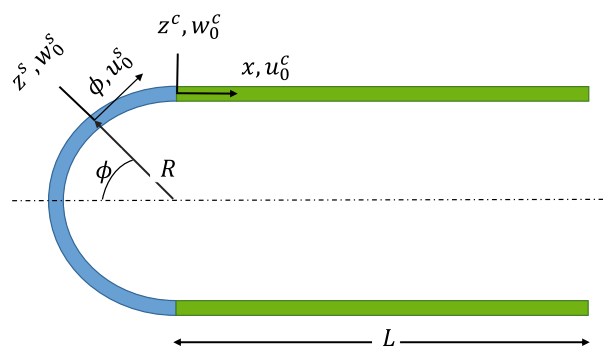
\includegraphics[width=0.75\textwidth]{vibro1_figure1.png}%
	\caption{Геометрические параметры и заданные системы координат объединенной цилиндрической и сферической оболочки}
	\label{fig:vibro1:1}
\end{figure}

\subsection{Описание свойств ФГМ} \label{ch:ch3/sec2/sub2}
Предполагается, что свойства материала керамической и металлической составляющих системы соединенных оболочек распределены по толщине на основе степенной функции. Предполагается, что объемная доля керамики \(V_c\) и объемная доля металла \(V_m\) подчиняются следующей форме [29-36*].

\begin{equation}
	\label{eq:vibro1:1}
	V_c = \left (\frac{1}{2}+\frac{z}{h} \right )^{k} ,\quad  V_m =1 - V_c
\end{equation}


В приведенном выше уравнении \(k\) является показателем функции и диктует распределение свойств материала по толщине. Очевидно, что поверхность \(z = +h/2\) богата керамикой, а поверхность \(z = -h/2\) богата металлом.


Следуя простому правилу подхода смесей (правило Фойгта), каждое свойство объединенной оболочки FG, например P, может быть записано как функция соответствующих свойств составляющих и объемной доли составляющих как

\begin{equation}
	\label{eq:vibro1:2}
	P(z) = P_m + P_{cm} \left (\frac{1}{2}+\frac{z}{h} \right )^{k} ,\quad  P_{cm} = P_c - P_m
\end{equation}

где \(P_m\) и \(P_c\) -- соответствующие свойства металлических и3 керамических компонентов, соответственно. В настоящей работе предполагается, что модуль упругости E и плотность массы \(\rho \) описываются уравнением (\cref{eq:vibro1:2}), а коэффициент Пуассона \(\mu \) считается постоянным по всей толщине, поскольку он изменяется только в небольшом диапазоне.


\subsection{Постановка задачи}\label{ch:ch3/sec2/sub3}

Рассмотрим объединенную цилиндрическо-полусферическую оболочку из функционально-градиентного материала равномерной толщины \(h\), радиуса сферы \(r^s = R\), радиуса цилиндра \(r^c = R\) и длины цилиндра \(L^c = L\). Система показана на \cref{fig:vibro1:1}. Система координат \((x, \theta, z)\) применяется к системе цилиндрической оболочки, а система \((\phi, \theta, z)\) -- к сферической оболочке. Системы координат также показаны на \cref{fig:vibro1:1}.

Чтобы учесть деформации сдвига по толщине и эффекты вращательной инерции цилиндрических и сферических оболочек, для формулировки определяющих уравнений оболочки используется теория сдвиговых деформаций первого порядка (\textbf{FSDT}) оболочек. На основе FSDT компоненты смещения в общей точке для цилиндрических и сферических оболочек могут быть представлены в соответствии с характеристиками средней поверхности таким образом, что

\begin{equation}
	\label{eq:vibro1:3}
	\begin{split}
	u^i (\xi, \theta, z, t) &= u_0^i(\xi, \theta, t)+ z \varphi_{\xi}^i (\xi, \theta,  t)\\
	v^i (\xi, \theta, z, t) &= v_0^i(\xi, \theta, t)+ z \varphi_{\theta}^i (\xi, \theta,  t)\\
	w^i (\xi, \theta, z, t) &= w_0^i (\xi, \theta, t)
	\end{split}
\end{equation}

В приведенном выше уравнении \(u, v, w\) -- это тангенциальное, окружное и поперечное перемещения по толщине, соответственно. Надстрочный индекс \(i\) может быть \(c\) или \(s\) для цилиндрических и сферических оболочек. Кроме того, \(\xi\) может принимать значение \(\phi\) или \(x\) для сферических и цилиндрических оболочек, соответственно. Подстрочный индекс 0 указывает на характеристики срединной поверхности. Кроме того, \(\phi_{\xi}\) и \(\phi_{\theta}\)  -- это, соответственно, повороты поперечных нормалей вокруг осей \(\theta\) и \(\xi\), соответственно.

Согласно FSDT, компоненты поля деформации в произвольной точке цилиндрической или сферической оболочки могут быть получены в терминах срединной поверхности оболочки и изменению кривизны.  Следовательно, можно записать [37*]

\begin{equation}
	\label{eq:vibro1:4}
	\begin{Bmatrix}
		\varepsilon_{\xi \xi}^i \\
		\varepsilon_{\theta \theta}^i \\
		\gamma_{\xi \theta}^i \\
		\gamma_{\xi z}^i \\
		\gamma_{\theta z}^i
	\end{Bmatrix} =
	\begin{Bmatrix}
		\varepsilon_{\xi \xi 0}^i \\
		\varepsilon_{\theta \theta 0}^i \\
		\gamma_{\xi \theta 0}^i \\
		\gamma_{\xi z 0}^i \\
		\gamma_{\theta z 0}^i
	\end{Bmatrix}
	+ z
		\begin{Bmatrix}
			\kappa_{\xi \xi}^i \\
			\kappa_{\theta \theta}^i \\
			\kappa_{\xi \theta}^i \\
			\kappa_{\xi z}^i \\
			\kappa_{\theta z}^i
	\end{Bmatrix}
\end{equation}

где компоненты деформации, связанные со средней поверхностью цилиндрической оболочки, имеют вид

\begin{equation}
\label{eq:vibro1:5}
\begin{Bmatrix}
		\varepsilon_{\xi \xi 0}^{c} \\
		\varepsilon_{\theta \theta 0}^{c} \\
		\gamma_{\xi \theta 0}^{c} \\
		\gamma_{\xi z 0}^{c} \\
		\gamma_{\theta z 0}^{c}
\end{Bmatrix} =
\begin{Bmatrix}
		u_{0, x}^c \\
		\frac{v_{0, \theta}^c}{r^c}+\frac{w_{0}^c}{r^c} \\
		\frac{u_{0, \theta}^c}{r^c}+v_{0, x}^c \\
		w_{0,x}^c+\varphi_{x}^c \\
		\frac{w_{0,\theta}^c}{r^c}-\frac{v_{0}^c}{r^c} + \varphi_{\theta}^c
\end{Bmatrix}
\end{equation}


и аналогично для сферической оболочки получаем

\begin{equation}
	\label{eq:vibro1:6}
	\begin{Bmatrix}
		\varepsilon_{\phi \phi 0}^{s} \\
		\varepsilon_{\theta \theta 0}^{s} \\
		\gamma_{\phi \theta 0}^{s} \\
		\gamma_{\phi z 0}^{s} \\
		\gamma_{\theta z 0}^{s}
	\end{Bmatrix} =
	\begin{Bmatrix}
		\frac{u_{0, \phi}^s}{r^s}+\frac{w_{0}^s}{r^s} \\
		\frac{v_{0, \theta}^s}{r^s \sin{\phi}}+\frac{u_{0}^s}{r^s} \cot{\phi}+\frac{w_0^s}{r^s} \\
		\frac{v_{0, \phi}^s}{r^s} +\frac{u_{0}^s}{r^s \sin{\phi}} -\frac{v_0^s}{r^s}\cot{\phi}\\
		\frac{w_{0, \phi}^s}{r^s} +\varphi_{\phi}^s -\frac{u_0^s}{r^s} \\
		\frac{w_{0,\theta}^c}{r^c}-\frac{v_{0}^c}{r^c} + \varphi_{\theta}^c
	\end{Bmatrix}
\end{equation}

Компоненты изменения кривизны в смысле Доннелла, совместимые с FSDT для цилиндрической оболочки [37*]

\begin{equation}
	\label{eq:vibro1:7}
	\begin{Bmatrix}
		\kappa_{xx}^{c} \\
		\kappa_{\theta \theta}^{c} \\
		\kappa_{x \theta}^{c} \\
		\kappa_{x z}^{c} \\
		\kappa_{\theta z}^{c}
	\end{Bmatrix} =
	\begin{Bmatrix}
		\varphi_{x,x}^c \\
		\frac{\varphi_{\theta, \theta}^c}{r^c} \\
		\frac{\varphi_{x, \theta}^c}{r^c}+\varphi_{\theta, x}^c \\
		0 \\
		0
	\end{Bmatrix}
\end{equation}

а для сферической оболочки могут быть записаны в виде

\begin{equation}
	\label{eq:vibro1:8}
	\begin{Bmatrix}
		\kappa_{\phi\phi}^{s} \\
		\kappa_{\theta \theta}^{s} \\
		\kappa_{\phi \theta}^{s} \\
		\kappa_{\phi z}^{s} \\
		\kappa_{\theta z}^{s}
	\end{Bmatrix} =
	\begin{pmatrix}
		\frac{\varphi_{\phi,\phi}^s}{r^s} \\
		\frac{\varphi_{\theta, \theta}^s}{r^s \sin{\phi}} + \frac{\varphi_{\theta}^s}{r^s}\cot{\phi} \\
		\frac{\varphi_{\theta, \phi}^s}{r^s}+\frac{\varphi_{\phi, \theta}^s}{r^s \sin{\phi}}-\frac{1}{r^s}\varphi_{\theta}^s \cot{\phi} \\
		0 \\
		0
	\end{pmatrix}
\end{equation}


Для случая, когда свойства материала оболочки линейно упругие, компоненты напряжения в виде деформаций рассчитываются как 

\begin{equation}
	\label{eq:vibro1:9}
	\begin{Bmatrix}
		\sigma_{\xi \xi}^i \\
		\sigma_{\theta \theta}^i \\
		\tau_{\xi \theta}^i \\
		\tau_{\xi z}^i \\
		\tau_{\theta z}^i
	\end{Bmatrix} =
	\begin{bmatrix}
		Q_{11} & Q_{12} & 0       & 0  	  & 0 \\
		Q_{12} & Q_{22} & 0       & 0     & 0 \\
		 0     &     0  & Q_{44}  & 0 	  & 0 \\
		 0     &     0  & 0       & Q_{55}& 0 \\
		 0     &     0  & 0       & 0     &  Q_{66}
	\end{bmatrix}
	\begin{Bmatrix}
		\varepsilon_{\xi \xi}^i \\
		\varepsilon_{\theta \theta}^i \\
		\gamma_{\xi \theta}^i \\
		\gamma_{\xi z}^i \\
		\gamma_{\theta z}^i
	\end{Bmatrix}
\end{equation}

где \(Q_{ij}, i,j =1, 2, 4, 5, 6\) являются приведенными коэффициентами жесткости материала и получаются следующим образом

\begin{equation}
	\label{eq:vibro1:10}
	Q_{11} = Q_{22} = \frac{E(z)}{1-\nu^2}, \quad Q_{12}=\frac{\nu E(z)}{1-\nu^2}, \quad Q_{44}=Q_{55}=Q_{66}=\frac{E(z)}{2(1+\nu)}
\end{equation}

Компоненты результирующих напряжений получены с использованием компонентов напряжений как [38*]

\begin{equation}
	\label{eq:vibro1:11}
	\begin{split}
	\begin{Bmatrix}
		N_{\xi \xi}^{i} \\
		N_{\theta \theta}^{i} \\
		N_{\xi \theta}^{i} 
	\end{Bmatrix} &=
	\int_{-h/2}^{+h/2}
	\begin{Bmatrix}
		\sigma_{\xi \xi}^{i} \\
		\sigma_{\theta \theta}^{i} \\
		\tau_{\xi \theta}^{i} 
	\end{Bmatrix}
	dz,\\
	\begin{Bmatrix}
	M_{\xi \xi}^{i} \\
	M_{\theta \theta}^{i} \\
	M_{\xi \theta}^{i} 
\end{Bmatrix} &=
\int_{-h/2}^{+h/2} z
\begin{Bmatrix}
	\sigma_{\xi \xi}^{i} \\
	\sigma_{\theta \theta}^{i} \\
	\tau_{\xi \theta}^{i} 
\end{Bmatrix}
dz,\\
	\begin{Bmatrix}
	Q_{\xi z}^{i} \\
	Q_{\theta z}^{i}
\end{Bmatrix} &=
\int_{-h/2}^{+h/2} k
\begin{Bmatrix}
	\tau_{\xi z}^{i} \\
	\tau_{\theta z}^{i}
\end{Bmatrix}
dz
\end{split}
\end{equation}

В приведенном выше уравнении \(k\) -- это поправочный коэффициент сдвига FSDT. Как известно, принятие поправочного коэффициента сдвига приводит к более точной оценке собственных частот. Поскольку поправочный коэффициент сдвига зависит от граничных условий, свойств материала и типа нагрузки [39*], точное его значение определить не просто. Однако широко используются приблизительные значения \(k = 5/6 \) или \(k = \pi^2 / 12\). В данном исследовании коэффициент коррекции сдвига равен \(k = 5/6 \).


Подстановка \cref{eq:vibro1:11} в уравнение \cref{eq:vibro1:11} с одновременным использованием уравнений \cref{eq:vibro1:4}-\cref{eq:vibro1:8} дает результирующие напряжения в виде характеристик средней поверхности оболочки в виде

\begin{equation}
	\label{eq:vibro1:12}
	\begin{Bmatrix}
		N_{\xi \xi}^{i}\\
		N_{\theta \theta}^{i} \\
		N_{\xi \theta}^{i} \\
		M_{\xi \xi}^{i} \\
		M_{\theta \theta}^{i}\\
		M_{\xi \theta}^{i}\\
		Q_{\xi z}^{i}\\
		Q_{\theta z}^{i}	
	\end{Bmatrix} =
\begin{bmatrix}
	A_{11} & A_{12} & 0 & B_{11} & B_{12} & 0 & 0 & 0 \\
	A_{12} & A_{22} & 0 & B_{12} & B_{22} & 0 & 0 & 0 \\
	0 & 0 & A_{66} & 0 & 0 & 0 & 0 & 0 \\
	B_{11} & B_{12} & 0 & D_{11} & D_{12} & 0 & 0 & 0 \\
	B_{12} & B_{22} & 0 & D_{12} & D_{22} & 0 & 0 & 0 \\
	0 & 0 & 0 & 0 & 0 & D_{66} & 0 & 0 \\
	0 & 0 & 0 & 0 & 0 & 0 & k A_{44} & 0 \\
	0 & 0 & 0 & 0 & 0 & 0 & 0 & k A_{55}
\end{bmatrix}
	\begin{Bmatrix}
		\varepsilon_{\xi \xi 0}^{i}\\
		\varepsilon_{\theta \theta 0}^{i} \\
		\gamma_{\xi \theta 0}^{i} \\
		\kappa_{\xi \xi }^{i} \\
		\kappa_{\theta \theta}^{i}\\
		\kappa_{\xi \theta}^{i}\\
		\gamma_{\xi z 0}^{i}\\
		\gamma_{\theta z 0}^{i}
	\end{Bmatrix}
\end{equation}

В приведенном выше уравнении постоянные коэффициенты \(A_{i j} , B_{i j} и D_{i j}\) обозначают известные жесткости на растяжение, каплинга и изгиба, соответственно, которые рассчитываются по формуле

\begin{equation}
	\label{eq:vibro1:13}
	\left ( A_{i j} , B_{i j} и D_{i j} \right ) = \int_{-0.5 h}^{+0.5h} \left ( Q_{i j} , zQ_{i j} , z^2 Q_{i j} \right ) dz
\end{equation}

Полный набор уравнений движения и граничных условий объединенной системы цилиндрических и полусферических оболочек может быть получен на основе обобщенного принципа Гамильтона [38*]. Утверждение принципа Гамильтона гласит

\begin{equation}
	\label{eq:vibro1:14}
	\begin{split}
	\delta \int_{t_1}^{t_2} \left (K^i - \left ( U^i +V^i \right ) \right )\,dt = 0 \\
	\text{at } t=t_1,t_2: \delta u_0^i= \delta v_0^i=\delta w_0^i=\delta \varphi_{\xi}^i= \delta \varphi_{\theta}^i=0
	\end{split}
\end{equation}

где в приведенном выше уравнении \(\delta K^i\) -- виртуальная кинетическая энергия цилиндрической/сферической оболочки, которая равна

\begin{equation}
	\label{eq:vibro1:15}
	\delta K^i = \int_V^i \rho (z) \left ( \dot{u}^i \delta \dot{u}^i + \dot{v}^i \delta \dot{v}^i + \dot{w}^i \delta \dot{w}^i \right )\, dV^i
\end{equation} 
Тут точкой обозначена проихводная по времени. Поскольку \(\delta U^i\) виртуальная энергия деформации для цилиндрической/сферической оболочки, которая записывается следующим образом

\begin{equation}
	\label{eq:vibro1:16}
	\delta U^i = \int_V^i \left ( \sigma_{\xi \xi}^i \delta \varepsilon_{\xi \xi}^i + \sigma_{\theta \theta}^i \delta \varepsilon_{\theta \theta}^i +  \tau_{\xi \theta}^i \delta \gamma_{\xi \theta}^i + \kappa \tau_{\theta z}^i \delta \gamma_{\theta z}^i + \kappa \tau_{\xi z}^i \delta \gamma_{\xi z}^i \right ) \, dV^i
\end{equation}

А \(\delta V^i \) -- виртуальная потенциальная энергия внешних нагрузок, которая отсутствует для задачи свободных колебаний. Интегрирование вышеприведенных выражений по координате \(z\) и применение теоремы Грина-Гаусса для освобождения виртуальных градиентов перемещений приводит к выражениям для линейных уравнений движения цилиндрической и сферической оболочек, соответственно, в виде

\begin{equation}
	\label{eq:vibro1:17}
	\begin{split}
	N_{xx,x}^c &+ \frac{N_{x \theta,\theta}^c}{R} = I_1 \ddot{u}_0^i+I_2 \ddot{\varphi}_x^c
	\\
	\frac{N_{\theta \theta,\theta}^c}{R} &+ N_{x \theta,x}^c + \frac{Q_{\theta z}^c}{R} = I_1 \ddot{v}_0^i+I_2 \ddot{\varphi}_{\theta}^c
	\\
	Q_{xz,x}^c &+ \frac{Q_{\theta z,\theta}^c}{R} - \frac{N_{\theta \theta}^c}{R} = I_1 \ddot{w}_0^c
	\\
	M_{xx,x}^c &+ \frac{M_{x \theta, \theta}^c}{R} - Q_{xz}^c = I_2 \ddot{u}_0^c + I_3 \ddot{\varphi}_x^c
	\\
	M_{x \theta,x}^c &+ \frac{M_{\theta \theta, \theta}^c}{R} - Q_{\theta z}^c = I_2 \ddot{v}_0^c + I_3 \ddot{\varphi}_{\theta}^c
	\end{split}
\end{equation} 


\begin{equation}
	\label{eq:vibro1:18}
	\begin{split}
		\frac{N_{\phi \phi, \phi}^s}{R} &+ \frac{N_{\phi \theta,\theta}^s}{R\sin{\phi}} + \frac{N_{\phi \phi}^s - N_{\theta \theta}^s}{R} \cot{\phi} + \frac{Q_{\phi}}{r}= I_1 \ddot{u}_0^i+I_2 \ddot{\varphi}_x^c
		\\
		\frac{N_{\theta \theta, \theta}^s}{R \sin{\phi}} &+ \frac{N_{\phi \theta,\phi}^s}{R} + 2\frac{\cot{\phi}}{R} N_{\phi \theta}^s + \frac{Q_{\theta}^s}{R}= I_1 \ddot{v}_0^i+I_2 \ddot{\varphi}_{\theta}^c
		\\
		\frac{Q_{\phi z, \phi}^s}{R} &+ \frac{1}{R \sin{\phi}} Q_{\theta, \theta}^s + \frac{Q_{\phi}^s}{R}\cot{\phi}  - \frac{N_{\phi \phi}^s + N_{\theta \theta}^s}{R} = I_1 \ddot{w}_0^s
		\\
		\frac{M_{\phi \phi, \phi}^s}{R}&+\frac{M_{\phi \theta, \theta}^s}{R \sin{\phi}}+\frac{M_{\phi \phi}^s - M_{\theta \theta}^s}{R} \cot{\phi} - Q_{\phi}^s =I_2 \ddot{u}_0^s + I_3 \ddot{\varphi}_{\phi}^s
		\\
		\frac{M_{\theta \theta, \theta}^s}{R \sin{\phi}}&+\frac{M_{\phi \theta, \phi}^s}{R }+2\frac{\cot{\phi}}{R} M_{\phi \theta}^s - Q_{\phi}^s =I_2 \ddot{v}_0^s + I_3 \ddot{\varphi}_{\theta}^s
	\end{split}
\end{equation} 

В \cref{eq:vibro1:18} обозначение \(R\) используется как для \(r^c\), так и для \(r^s\). Также применяются следующие определения. В \cref{eq:vibro1:18} обозначение \(R\) используется как для \(r^c\), так и для \(r^s\). Кроме того, применяются следующие определения

\begin{equation}
	\label{eq:vibro1:19}
	\left ( I_1, I_2, I_3 \right ) = \int_{-h/2}^{+h/2} \rho (1, z, z^2)\, dz
\end{equation}

Для конца цилиндрической оболочки могут быть определены различные типы граничных условий. Край \(x = L\) может быть зажатым (C) или свободным (F). 


\subsection{Алгоритм поиска решения}\label{ch:ch3/sec2/sub4}

Ссылаясь на определения нормальной силы и изгибающего момента из уравнения \cref{eq:vibro1:12} и уравнений движения \cref{eq:vibro1:17} и \cref{eq:vibro1:18}, следующее разделение переменных точно удовлетворяет условиям периодичности полевых переменных, а также совместимо с уравнениями движения \cref{eq:vibro1:17} и \cref{eq:vibro1:18} и условиями соответствия \cref{eq:vibro1:22} и \cref{eq:vibro1:23}.

\begin{equation}
	\label{eq:vibro1:24}
	\begin{Bmatrix}
		u_0^i(\xi, \theta, t) \\
		v_0^i(\xi, \theta, t) \\
		w_0^i(\xi, \theta, t) \\
		\varphi_{\xi}^i(\xi, \theta, t) \\
		\varphi_{\theta}^i(\xi, \theta, t)
	\end{Bmatrix} =
	\cos({\omega t + \psi})
\begin{bmatrix}
	\sin{n \theta} & 0 & 0 & 0 & 0 \\
	0 & \cos{n \theta} & 0 & 0 & 0 \\
	0 & 0 & \sin{n \theta} & 0 & 0 \\
	0 & 0 & 0 & \sin{n \theta} & 0 \\
	0 & 0 & 0 & 0 & \cos{n \theta}
\end{bmatrix}
	\begin{Bmatrix}
		U^i(\xi) \\
		V^i(\xi) \\
		W^i(\xi) \\
		\Phi_{\xi}^i(\xi) \\
		\Phi_{\theta}^i(\xi)
	\end{Bmatrix}
\end{equation}

где в приведенном выше уравнении \(n\), как уже упоминалось, является волновым числом в окружном направлении. Временная зависимость решения \cref{eq:vibro1:24} выбрана для преодоления условия периодичности поля переменных во временной области. В этой функции \(\omega\) -- собственная частота объединенной системы оболочек.


Подстановка вышеприведенного уравнения в уравнения движения \cref{eq:vibro1:17} и \cref{eq:vibro1:18} приводит к новым десяти связанным обыкновенным дифференциальным уравнениям в терминах неизвестных сквозных меридианных функций \(U^i(\xi), V^i(\xi), W^i (\xi), \Phi_{\xi}^i, \Phi_{\theta}^i\). Преобразованные уравнения и соответствующие граничные условия для цилиндрического/сферического сегмента здесь не приводятся и представлены в "Приложении A".

Как и ожидалось, уравнения (A.1)-(A.10) вместе с правильным выбором граничных и согласующих условий приводят к системе однородных уравнений. Чтобы решить систему уравнений как задачу на собственные значения, применяется метод GDQ для преобразования обыкновенных дифференциальных уравнений (A.1)-(A.10) в новые линейные алгебраические уравнения. Метод GDQ достаточно хорошо известен, и его детали здесь не повторяются. Между тем, за более подробной информацией можно обратиться к [41*]. Стоит отметить, что распределение узловых точек в каждом сегменте описывается с помощью точек Чебышева-Гаусса-Лобатто, что приводит к следующим результатам

Известны четыре общие процедуры для наложения граничных условий на дискретизированную систему на основе GDQ. В данном исследовании для применения граничных и согласующих условий используется метод SBCGE, который непосредственно подставляет граничные условия в управляющие уравнения. Основываясь на этой технике, необходимо применить метод GDQ как к уравнениям движения, так и к граничным условиям. Уравнения движения после дискретизации, применения согласующих и граничных условий и глобальной ассемблировки принимают вид

\begin{equation}
\label{eq:vibro1:26}
\boldsymbol{K } \Delta = \omega^2 \boldsymbol{M} \Delta
\end{equation}

где в приведенном выше уравнении \(M\) -- обобщенная матрица масс, \(K\) -- обобщенная матрица жесткости и неизвестный вектор перемещения. Собственные частоты конструкции могут быть получены путем решения стандартной задачи на собственные значения \cref{eq:vibro1:26}.

\subsection{Вывод для данного решения}\label{ch:ch3/sec2/sub5}

 данном исследовании оценивается отклик свободных колебаний объединенной системы цилиндрической и полусферической оболочек. Предполагается, что оболочка изготовлена из FGM, свойства которого градируются в направлении толщины. Для описания объемной доли компонентов используется простая функция степенного закона, а для оценки свойств применяется простое правило смесей Фойгта. Для создания управляющих уравнений системы оболочек используется теория оболочек сдвиговой деформации первого порядка и кинематические предположения типа Доннелла. Используя принцип Гамильтона, получен полный набор управляющих уравнений и граничных условий для оболочек. С помощью разложения Фурье по окружности и метода GDQ для управляющих уравнений, граничных условий и условий согласования пересечений получена полная система алгебраических уравнений, которая решается как задача с собственными значениями. После проверки результатов данного исследования для случая однородных оболочек, получены новые численные результаты для случая оболочек FGM. Показано, что индекс силового закона FGM, отношение радиуса к длине цилиндрической оболочки и отношение длины к радиусу являются важными факторами, влияющими на частоты объединенной системы оболочек.
 
\section{Автоколебания пластины из ФГМ под действием быстрого нагрева} \label{ch:ch3/sec3}

\subsection{Обзор}\label{ch:ch3/sec3/sub1}
В данной части работы анализируется термоиндуцированная вибрация кольцевой секторной пластины из функционально-градиентных материалов. Считается, что все термомеханические свойства среды FGM зависят от температуры. На основе теории линейной термоупругости без связи устанавливается одномерное переходное уравнение теплопроводности типа Фурье. Верхняя и нижняя поверхности пластины находятся под различными типами граничных условий быстрого нагрева. Из-за зависимости свойств материала от температуры уравнение теплопроводности становится нелинейным. Поэтому необходимо использовать численный метод. Сначала для дискретизации уравнения теплопроводности по толщине пластины применяется метод обобщенных дифференциальных квадратур (\textbf{GDQM}). Затем, управляющая система зависящих от времени обыкновенных дифференциальных уравнений решается с помощью метода последовательного марширования по времени Крэнка-Николсона. Полученные результирующие тепловой силы и теплового момента на каждом временном шаге от температурного профиля применяются к уравнениям движения. Уравнения движения, основанные на теории деформации сдвига первого порядка (\textbf{FSDT}), получены с помощью принципа Гамильтона. С помощью GDQM двумерная область секторной пластины и подходящих граничных условий разбивается на ряд узловых точек, а дифференциальные уравнения превращаются в систему обыкновенных дифференциальных уравнений. Для получения неизвестного вектора смещения в любой момент времени используется метод прямого интегрирования, основанный на маршевой схеме Ньюмарка по времени. Для проверки формулировки и метода решения в настоящем исследовании проводятся сравнительные исследования. На различных примерах рассматривается влияние таких эффективных параметров, как показатель степени в зависимости FGM, толщина пластины, зависимость от температуры, угол раскрытия сектора, значения радиуса, граничные условия в плоскости и тип граничных условий быстрого нагрева на термоиндуцированный отклик пластины FGM при тепловом ударе.


Исследования термоиндуцированного отклика тонких конструктивных элементов в основном можно разделить на квазистатические и динамические исследования. Первые работы по теме термоиндуцированных колебаний принадлежат Болею [1**, 2**]. Болей [1**] исследовал динамический отклик быстро нагретой изотропной тонкой балки. В этом исследовании результаты показали, что параметр инерции, который зависит от геометрии и термомеханических свойств, является основным фактором. Боли и Барбер [2**] также проанализировали быстрый нагрев прямоугольных просто поддерживаемых пластин. Аналитические ряды Фурье используются для получения отклика пластины. Краус [3**] исследовал термоиндуцированную вибрацию сферических оболочек. Предполагается, что оболочка находится под тепловым ударом на одной поверхности, в то время как другая поверхность теплоизолирована. Он подтвердил важность параметра инерции для вибрационного поведения тонких оболочек при тепловом ударе.  Другим основным результатом его исследования является то, что из-за связи растяжения-изгиба в кинематике оболочек, параметр инерции в балках играет более определяющую роль, чем в пластинах и оболочках, соответственно. Страуд и Майерс [4**] использовали модифицированный вариационный принцип энергии Рейсса для изучения влияния зависимости от температуры на термоиндуцированные колебания пластин, подвергнутых произвольному тепловому удару. Исходя из полученных результатов, игнорирование температурной зависимости свойств материала приводит к ошибочным результатам в термоиндуцированной реакции пластин при тепловом ударе.


Осесимметричный динамический прогиб круглых пластин при быстром нагреве рассмотрен Накаджо и Хаяши [5**]. Они исследовали термоиндуцированную вибрацию на основе экспериментальных, аналитических и численных методов, используя линейные и нелинейные соотношения деформации и перемещения. Как было замечено в этом исследовании, для специальных граничных условий, основанных на линейной теории, пластина демонстрирует различные реакции, полученные экспериментальным и теоретическим методами. Киани и Эслами [6**] проанализировали нелинейную термоиндуцированную вибрацию функционально-градиентных круглых пластин на основе геометрической нелинейности типа фон Кармана. Предполагается, что термоупругие свойства материала зависят от температуры. Они сообщили, что конструкции без начальной кривизны с зажатыми краями способны компенсировать дополнительные моменты для сохранения прямолинейного состояния до определенного времени, в течение которого наступает динамическая неустойчивость и конструкция вибрирует. Эслами [7**] в учебнике проанализировал нелинейную динамическую тепловую неустойчивость различных типов тонких структур на основе нескольких методов.


В работе Venkataramana и Jana [8**] анализируется быстрый нагрев изотропной балки, подверженной гармоническому изменению температуры. Отклик балки получен в двух частях: статической и динамической. В вышеупомянутом исследовании, основанном на процедуре суперпозиции, полный прогиб имеет тенденцию колебаться вокруг статической реакции. Кидава-Кукла [9**] использовал схему функции Грина для обсуждения вынужденных колебаний балок, подверженных воздействию движущегося концентрированного источника тепла. В этом исследовании рассматриваются эффекты внутреннего и внешнего демпфирования на поперечный отклик. Брух и др. [10**] разработали стратегию активного управления для уменьшения максимальной деформации и скорости просто поддерживаемой быстро нагреваемой балки.  Влияние сжимающих нагрузок в плоскости и внутреннего/внешнего демпфирования на тепловые прогибы балочных конструкций описано Манолисом и Бескосом [11**]. Решение уравнения колебательного движения во временной области получено с помощью метода численного преобразования Лапласа. Адам и др. [12**] исследовали эффект межслойного скольжения на тепловой отклик вязкоупругих композитных балок Эйлера-Бернулли. Разделив динамическую реакцию на квазистатическую и дополнительную динамическую части, получена реакция балки при быстром нагреве. Квазистатическое решение определено в замкнутой форме, а оставшаяся дополнительная динамическая часть получена численно с помощью усеченного модального ряда. Явление теплового флаттера изотропных консольных балок при солнечном нагреве проанализировано Чжаном и другими [13**]. Они ввели критерий, согласно которому тепловой флаттер может возникнуть, если угол распространения солнечного теплового потока меньше угла изгиба свободного края, когда балка находится в квазистатическом равновесии. Малик и Кадоли [14**] исследовали термоиндуцированную вибрацию балок из FGM при различных типах быстрого нагрева. Предполагается, что одна поверхность балки подвергается воздействию движущейся нагревательной нагрузки, ступенчатого нагрева, ударного нагрева и сосредоточенного линейного источника тепла, а противоположная поверхность термически изолирована или подвергается конвективным потерям тепла. Основываясь на методе Ритца и используя теорию деформации сдвига первого порядка, Гиасян и др. [15**] исследовали нелинейный тепловой прогиб быстро нагреваемой балки ФГМ. Все свойства материала считаются зависящими от температуры


Таухерт [16**] исследовал термоиндуцированную вибрацию ортотропных прямоугольных пластин с различными типами граничных условий, связанных с краевыми опорами типа Леви.  Применяя метод комплексных переменных к уравнениям движения, Дас [17**] проанализировал термоиндуцированную реакцию пластин произвольной многоугольной формы, подвергнутых тепловому удару.  Влияние пьезо-термоупругих слоев на подавление реакции прямоугольных и круглых пластин при тепловом ударе исследовано Таухертом и др [18**]. Чанг и др. [19**] провели исследование для получения отклика быстроударных слоистых композитных пластин с использованием двумерного вариационного метода конечных элементов. Для аппроксимации полей перемещений используется теория высшего порядка, учитывающая поперечные сдвиговые и нормальные деформации. Алипур и др. [20**] исследовали термоиндуцированную реакцию квадратных пластин с учетом положения и зависящих от температуры свойств материала. Для дискретизации уравнений движения применяется двумерный обобщенный дифференциальный квадратичный метод.  С помощью хорошо известного метода Рунге-Кутты четвертого порядка был получен отклик пластины. Джавани и др. исследовали геометрически нелинейный тепловой прогиб кольцевой пластины ФГМ [21**], неглубоких арок [22**], сферических оболочек [23**] и конических оболочек [24**] с зависящими от температуры свойствами материала, используя метод дифференциальных квадратур.


Хилл и Мазумдар [25**] предложили методику для теплового прогиба вязкоупругих пластин и тонких оболочек, испытывающих большие прогибы. Метод решения в основном заимствован из предыдущих исследований авторов для типа связей деформация-перемещение [26-28**]. Однако методология решения может быть применима даже для прогибов, которые находятся в диапазоне толщины конструкции. Быстро нагревающиеся поперечные слоистые трубы исследованы на основе двумерного метода GDQ Хонгом и другими [29**]. Esmaeili и др. [30**] представили осесимметричные термоиндуцированные колебания большой амплитуды цилиндрических оболочек из материала FG, зависящего от температуры, используя метод Ритца. Хуанг и Таухерт [31**] исследовали быстрый нагрев композитных панелей. Решение Навье применяется для получения теплового прогиба просто поддерживаемых поперечных симметричных и антисимметричных ламинированных панелей двойной кривизны.  Геометрически нелинейные деформации цилиндрических панелей с использованием теории фон Кармана при тепловых ударах исследованы Хуангом и Таухертом [32**]. В этом исследовании используется двумерный метод конечных элементов. Кейболахи и др. [33**] продемонстрировали, что при некоторых особых геометрических и граничных условиях динамическое термическое смятие тонких шалевых арок происходит при термоиндуцированной вибрации. Используя метод Ритца и критерий Будянского-Хатчинсона, была получена критическая температура. Кейболахи и др. [34**] развили предыдущую работу для анализа нелинейного быстрого нагрева неглубоких арок с различными типами граничных условий. Основываясь на классической теории оболочек, Хдейр [35**, 36**] сообщил о термоиндуцированной реакции неглубоких оболочек и арок, подверженных быстрому нагреву, используя аналитический метод.  Путем внедрения связанной и несвязанной теорий термовязкости в уравнения движения быстро нагружаемых толстых круговых цилиндрических слоистых композитных оболочек Чанг и Шьонг [37**] проанализировали тепловую реакцию с помощью метода конечных элементов. Управление тепловым прогибом в пьезо-гигро-термоупругих слоистых пластинах и оболочках выполнено Раджа и др [38**]. Также Кумар и др. [39] исследовали вынужденные колебания пьезо-ламинированных тонких цилиндрических оболочек под электрическими, механическими и тепловыми нагрузками с помощью метода конечных элементов.  Пандей и Прадьюмна [40**] проанализировали многослойные пластины FGM и двояковогнутые панели при быстром нагреве.  В данном исследовании рассматривается теория слоев высшего порядка.


В настоящем исследовании впервые исследуется термоиндуцированная вибрация зависящей от температуры кольцевой секторной пластины из ФГМ с произвольными граничными условиями. Предполагается, что термомеханические свойства пластины зависят от температуры. Нелинейное уравнение теплопроводности типа Фурье с граничными условиями быстрого нагрева в верхней и боковой плоскостях решается одномерным обобщенным методом квадратурных разностей (\textbf{GDQM}) и маршевой схемой Кранка-Никольсона. С помощью теории сдвиговой деформации пластин первого порядка и двумерного GDQM получены матрицы упругой жесткости и массы, а также вектор силы секторной пластины. Система зависящих от времени обыкновенных дифференциальных уравнений решается с помощью гибридного метода Ньюмарка-Ньютона-Рафсона для получения профиля бокового прогиба секторной пластины во временной области. Сравнительное исследование позволяет убедиться в эффективности и точности разработанной методики. Представлено влияние различных параметров на термоиндуцированный прогиб быстроударной кольцевой секторной пластины.


\subsection{Медель материала пластины}\label{ch:ch3/sec3/sub2}

\begin{figure}[h!]
	\centering
	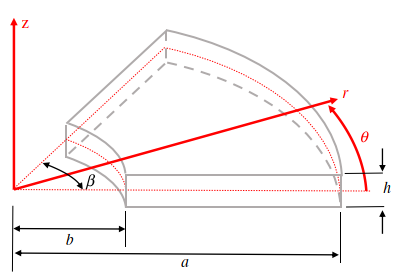
\includegraphics[width=0.75\textwidth]{vibro2_figure1.png}%
	\caption{Схема и локальная СК для сектора из ФГМ}
	\label{fig:vibro2:1}
\end{figure}

Рассмотрим металлокерамическую функционально-градиентную кольцевую секторную пластину внутреннего радиуса \(b\), внешнего радиуса \(a\) и толщины \(h\). Как показано на \cref{fig:vibro2:1}, задана система полярных координат \((r, \theta, z\)) с началом координат в центре средней плоскости секторной пластины.  Как обычно, \((r, \theta, z\)) показывают радиальное, окружное и поперечное направления, соответственно.


Эффективные термомеханические свойства кольцевой секторной пластины FGM могут быть определены в соответствии с надлежащей процедурой гомогенизации. Правило смеси Войгта обычно используется из-за его простоты и эффективности [41**-48**]. Согласно этому правилу, механические и тепловые характеристики пластины FGM, такие как модуль Юнга \(E\),  \(\nu\)коэффициент Пуассона, \(\alpha\)коэффициент теплового расширения, \(\rho\) массовая плотность, удельная теплоемкость \(C_v\) и теплопроводность \(K\), считаются линейными функциями объемных долей керамики \(V_c\) и металла \(V_m\). Таким образом, как функция направления толщины, неоднородное свойство пластины, \(P\), может быть выражено в виде [49**]

\begin{equation}
	\label{eq:vibro2:1}
	\begin{split}
	P(z, T) &= P_m(T) + V_c (z) P_{cm}(T)\\
	P_{cm}(T) &= P_c(T) - P_m(T)
	\end{split}
\end{equation}

Температурная зависимость составляющих ФГМ часто выражается на основе формулы Тулукиана. Соответственно, каждое свойство металла или керамики может быть записано в форме [49**]

\begin{equation}
	\label{eq:vibro2:2}
		P(T) = P_0 \left (P_{-1}T^{-1}+1+P_1 T^1 + P_2 T^2 + P_3 T^3 \right )
\end{equation}

В котором \(T\) -- температура, измеренная в Кельвинах, а \(P^i\) -- константы, уникальные для каждого компонента. Придерживаясь обозначений Редди и Чину [49**], для представления объемной доли керамики \(V_c\) и объемной доли металла \(V_m\) можно использовать распределение по степенному закону в направлении толщины так, что

\begin{equation}
	\label{eq:vibro2:3}
	V_c = \left ( \frac{1}{2} + \frac{z}{h} \right ) ^{\xi}, \quad V_m = 1 - V_c
\end{equation}
Здесь \(\xi\) -- неотрицательный показательстепени, определяющий профиль дисперсии свойств.

\subsection{Постановка задачи}\label{ch:ch3/sec3/sub3}

Численные результаты данного исследования ограничиваются оценкой бокового прогиба на основе теории сдвиговых деформаций первого порядка (\textbf{FSDT}). Согласно двумерной FSDT, смещения общей точки секторной пластины характеризуются в терминах смещений средней поверхности как:

\begin{equation}
	\label{eq:vibro2:4}
	\begin{split}
		u^i (r, \theta, z, t) &= u_0^i(r, \theta, t)+ z \varphi_{r}^i (r, \theta,  t)\\
		v^i (r, \theta, z, t) &= v_0^i(r, \theta, t)+ z \varphi_{\theta}^i (r, \theta,  t)\\
		w^i (r, \theta, z, t) &= w_0^i (r, \theta, t)
	\end{split}
\end{equation}
где \(u, v, w\)) -- перемещение срединной поверхности в трех направлениях. \( \varphi_{r}, \varphi_{\theta} \) -- обозначают продольные вращения вокруг осей \( \theta, r\).


Компоненты деформации, связанные с полями перемещений \cref{eq:vibro2:4}, согласно теории кольцевых секторных пластин, могут быть представлены в виде:

\begin{equation}
	\label{eq:vibro1:5}
	\begin{split}
		\varepsilon_{rr} &= u_{0, r}
		\\
		\varepsilon_{\theta \theta } &= \frac{u}{r}+\frac{v{,\theta}}{r}
		\\
		\gamma_{r \theta} &= \frac{u_{, \theta}}{r}+v_{, r} - \frac{1}{r}v
		\\
		\gamma_{r z } &= u_{,z}+w_{,r}
		\\
		\gamma_{\theta z} &= v_{,z}-\frac{1}{r} w_{,\theta} 
	\end{split}
\end{equation}

где эпсилон это соответсвующее перемещение, а гамма это сдвиг. Запятая обозначает производную.

Рассматриваем \(T \)и \(T_0\) как распределение температуры и температуру начала отсчета и предполагая линейный термоупругий материал (закон Гука), определяющий закон для секториальной пластины ФГМ, подверженной тепловым нагрузкам, имеет вид

\begin{equation}
	\label{eq:vibro2:6}
	\begin{Bmatrix}
		\sigma_{\xi \xi}^i \\
		\sigma_{\theta \theta}^i \\
		\tau_{\xi \theta}^i \\
		\tau_{\xi z}^i \\
		\tau_{\theta z}^i
	\end{Bmatrix} =
	\begin{bmatrix}
		Q_{11} & Q_{12} & 0       & 0  	  & 0 \\
		Q_{12} & Q_{22} & 0       & 0     & 0 \\
		0     &     0  & Q_{44}  & 0 	  & 0 \\
		0     &     0  & 0       & Q_{55}& 0 \\
		0     &     0  & 0       & 0     &  Q_{66}
	\end{bmatrix}
	\left (
	\begin{Bmatrix}
		\varepsilon_{\xi \xi}^i \\
		\varepsilon_{\theta \theta}^i \\
		\gamma_{\xi \theta}^i \\
		\gamma_{\xi z}^i \\
		\gamma_{\theta z}^i
	\end{Bmatrix}
	- (T-T_0))
		\begin{Bmatrix}
		\alpha \\
		\alpha \\
		0 \\
		0 \\
		0
	\end{Bmatrix}
	\right )
\end{equation}

где \(Q_{ij}, i,j =1, 2, 4, 5, 6\) являются приведенными коэффициентами жесткости материала и получаются следующим образом

\begin{equation}
	\label{eq:vibro2:7}
	\begin{split}
	Q_{11} = Q_{22} &= \frac{E(z, T)}{1-\nu^2(z, T)}, \quad Q_{12}=\frac{\nu(z, T) E(z, T)}{1-\nu^2(z,T)}
	\\
	Q_{66}&=\frac{E(z, T)}{2(1+\nu(z, T))} \quad Q_{44}=Q_{55}=kQ_{66}
	\end{split}
\end{equation}
где \(k=5/6\) как было выбрано ранее.

Используя FSDT, результирующие напряжения мембраны \(N_{rr}, N_{\theta \theta}, и N_{r \theta}\), результирующие напряжения сдвига вне плоскости мембраны\( Q_r , Q_{\theta},\) и результирующие напряжения изгиба \(M_{rr}, M_{\theta, \theta}, M_{r \theta}\) могут быть представлены при интегрировании компонентов напряжения как


\begin{equation}
	\label{eq:vibro2:8}
	\begin{split}
		\begin{Bmatrix}
			N_{r r}^{i} \\
			N_{\theta \theta}^{i} \\
			N_{ \theta}^{i} 
		\end{Bmatrix} &=
		\int_{-h/2}^{+h/2}
		\begin{Bmatrix}
			\sigma_{r \xi}^{i} \\
			\sigma_{\theta \theta}^{i} \\
			\tau_{r \theta}^{i} 
		\end{Bmatrix}
		dz,\\
		\begin{Bmatrix}
			M_{rr}^{i} \\
			M_{\theta \theta}^{i} \\
			M_{r \theta}^{i} 
		\end{Bmatrix} &=
		\int_{-h/2}^{+h/2} z
		\begin{Bmatrix}
			\sigma_{rr}^{i} \\
			\sigma_{\theta \theta}^{i} \\
			\tau_{r \theta}^{i} 
		\end{Bmatrix}
		dz,\\
		\begin{Bmatrix}
			Q_{r}^{i} \\
			Q_{\theta}^{i}
		\end{Bmatrix} &=
		\int_{-h/2}^{+h/2} k
		\begin{Bmatrix}
			\tau_{r z}^{i} \\
			\tau_{\theta z}^{i}
		\end{Bmatrix}
		dz
	\end{split}
\end{equation}

Подставляя \cref{eq:vibro2:6} в \cref{eq:vibro2:8} с помощью уравнений \cref{eq:vibro2:4} и \cref{eq:vibro2:5}, результирующие напряжения в компонентах смещения получаются как \cref{eq:vibro1:12} с учетом еще одного члена.

\begin{equation}
	\label{eq:vibro2:9}
	\begin{Bmatrix}
		N_{\xi \xi}^{i}\\
		N_{\theta \theta}^{i} \\
		N_{\xi \theta}^{i} \\
		M_{\xi \xi}^{i} \\
		M_{\theta \theta}^{i}\\
		M_{\xi \theta}^{i}\\
		Q_{\xi z}^{i}\\
		Q_{\theta z}^{i}	
	\end{Bmatrix} =
	-
		\begin{Bmatrix}
		N^{T}\\
		N^{T} \\
		0\\
		M^{T}\\
		M^{T}\\
		0\\
		0\\
		0	
	\end{Bmatrix}
	+
	\begin{bmatrix}
		A_{11} & A_{12} & 0 & B_{11} & B_{12} & 0 & 0 & 0 \\
		A_{12} & A_{22} & 0 & B_{12} & B_{22} & 0 & 0 & 0 \\
		0 & 0 & A_{66} & 0 & 0 & 0 & 0 & 0 \\
		B_{11} & B_{12} & 0 & D_{11} & D_{12} & 0 & 0 & 0 \\
		B_{12} & B_{22} & 0 & D_{12} & D_{22} & 0 & 0 & 0 \\
		0 & 0 & 0 & 0 & 0 & D_{66} & 0 & 0 \\
		0 & 0 & 0 & 0 & 0 & 0 & k A_{55} & 0 \\
		0 & 0 & 0 & 0 & 0 & 0 & 0 & k A_{55}
	\end{bmatrix}
	\begin{Bmatrix}
		\varepsilon_{rr}^{i}\\
		\varepsilon_{\theta \theta} \\
		\gamma_{r \theta} \\
		\kappa_{r r} \\
		\kappa_{\theta \theta}\\
		\kappa_{r \theta}\\
		\gamma_{r z }\\
		\gamma_{\theta z}
	\end{Bmatrix}
\end{equation}


В приведенном выше уравнении постоянные коэффициенты \(A_{i j} , B_{i j} и D_{i j}\) обозначают известные жесткости на растяжение, каплинга и изгиба, соответственно, которые рассчитываются по формуле \cref{eq:vibro1:13}

\begin{equation}
	\label{eq:vibro2:10}
	\left ( A_{i j} , B_{i j} и D_{i j} \right ) = \int_{-0.5 h}^{+0.5h} \left ( Q_{i j} , zQ_{i j} , z^2 Q_{i j} \right ) dz
\end{equation}

Кроме этого термальные погонные силы и моменты расчитываются по формуле

\begin{equation}
	\label{eq:vibro2:11}
	\left ( N^T, M^T \right ) = \int_{-0.5 h}^{+0.5 h} \left ( 1 z \right ) \frac{1}{1-\nu(z, T)} E(z, T) \alpha(z, T) (T-T_0) \, dz
\end{equation}


Уравнения движения предполагаемой кольцевой секторной пластины в предположении теории несвязанной термоупругости можно получить с помощью принципа Гамильтона [**7].  Соответственно, можно записать в виде \cref{eq:vibro1:14}

\begin{equation}
	\label{eq:vibro2:12}
		\delta \int_{t_1}^{t_2} \left (K^i - \left ( U^i +V^i \right ) \right )\,dt = 0
\end{equation}


Виртуальная потенциальная энергия и энергия деформации в полярных координатах запишется по аналогии с \cref{eq:vibro1:15} и \cref{eq:vibro1:16} в следующем виде:

Виртуальная энергия деформации
\begin{equation}
	\label{eq:vibro2:13}
	\delta U = \int_0^{\beta} \int_b^{a}  \int_{-0.5h}^{+0.5h}  \left ( \sigma_{rr} \delta \varepsilon_{rr} + \sigma_{\theta \theta} \delta \varepsilon_{\theta \theta} +  \tau_{r \theta} \delta \gamma_{r \theta} + \tau_{\theta z} \delta \gamma_{\theta z} +  \tau_{r z} \delta \gamma_{r z} \right ) r\, dz dr d\theta
\end{equation}
 
По аналогии, \(\delta V\) потенциальная энергия внешних сил отсутсвует. А кинетическая энергия записывается в ввиде


\begin{equation}
	\label{eq:vibro2:14}
	\begin{split}
	\delta K &= \int_0^{\beta} \int_b^{a}  \int_{-0.5h}^{+0.5h}   \rho (z, T)  ( \dot{u} \delta \dot{u} +  \dot{v} \delta \dot{v} +  \dot{w} \delta \dot{w} )  r\, dz dr d\theta
	\\
	&=\int_0^{\beta} \int_b^{a}   (  (I_1 \ddot{u} + I_2 \ddot{\varphi}_r)\delta u +(I_1 \ddot{v} + I_2 \ddot{\varphi}_{\theta}) \delta v +I_1 \ddot{w} \delta w + (I_2 \ddot{u} + I_3 \ddot{\varphi}_r) \delta \phi_r
	\\
	 &+(I_2 \ddot{v} + I_3 \ddot{\varphi}_{\theta}) \delta \varphi_{\theta}  )  r\, dz dr d\theta
	\end{split}
\end{equation}

\begin{equation}
	\label{eq:vibro2:15}
	\left ( I_1, I_2, I_3 \right ) = \int_{-h/2}^{+h/2} \rho(z, T) (1, z, z^2)\, dz
\end{equation}

Подставляя \cref{eq:vibro2:13} и \cref{eq:vibro2:14} в уравнение \cref{eq:vibro2:12} и используя соответствующие математические упрощения, выражения для уравнений движения кольцевой секторной пластины принимают вид

\begin{equation}
	\label{eq:vibro2:16}
	\begin{split}
	\delta u :\quad	N_{rr,r} &+ \frac{N_{r \theta,\theta}}{r} + \frac{1}{r} (N_{rr} - N_{\theta \theta})= I_1 \ddot{u}^i+I_2 \ddot{\varphi}_r
		\\
	\delta v : \quad	\frac{N_{\theta \theta,\theta}}{r} &+ N_{r \theta,r} + \frac{2}{r}N_{r \theta} = I_1 \ddot{v}+I_2 \ddot{\varphi}_{\theta}^c
		\\
	\delta w: \quad	Q_{r,r} &+ \frac{Q_{\theta ,\theta}}{r} + \frac{Q_{r}}{r} = I_1 \ddot{w}
		\\
	\delta \varphi_{r}:\quad	M_{rr,r} &+ \frac{M_{r \theta, \theta} }{r} +\frac{1}{r}(M_{rr} - M_{\theta \theta})- Q_{r} = I_2 \ddot{u} + I_3 \ddot{\varphi}_r
		\\
	\delta \varphi_{\theta} :\quad	M_{r \theta,r}  &+ \frac{M_{\theta \theta, \theta} }{r} - Q_{\theta } +\frac{2}{r} M_{r \theta}  = I_2 \ddot{v} + I_3 \ddot{\varphi}_{\theta}
	\end{split}
\end{equation} 

Основные уравнения движения в терминах компонентов перемещения для секторной пластины FGM можно получить с помощью уравнений \cref{eq:vibro2:9} и \cref{eq:vibro2:16}. Полученные уравнения имеют вид
{\color{blue} в приложении Б }

\subsection{Метод дискретизации GDQ}\label{ch:ch3/sec3/sub4}
Полученные первые и вторые производные функции \(f\) на сетке записываются в виде ряда значений на узлах самой сетки

\begin{equation}
	\label{eq:vibro2:20}
	\begin{split}
		\frac{\partial f}{\partial r} \Big |_{r=r_i, \theta=\theta_j} & = \sum_{m=1}^{N_r} \sum_{n=1}^{N_{\theta}} A_{im}^r I_{jn}^{\theta} f_{mn}
		\\
		\frac{\partial^2 f}{\partial r^2} \Big |_{r=r_i, \theta=\theta_j} & = \sum_{m=1}^{N_r} \sum_{n=1}^{N_{\theta}} B_{im}^r I_{jn}^{\theta} f_{mn}
	\end{split}
\end{equation}
 и другие в {\color{blue} в приложении Б }
 
 
\subsection{Метод решения}\label{ch:ch3/sec3/sub5}

Полученные дискретизированные уравнений движения  вместе с надлежащим выбором граничных условий могут быть записаны в компактной форме как

\begin{equation}
	\label{eq:vibro2:33}
	\left [ \boldsymbol{M(T)}\right ]  \left \{ \boldsymbol{\ddot{X}} \right \} + \left [ \boldsymbol{K(T)}\right ]  \left \{ \boldsymbol{X} \right \} = \left \{ \boldsymbol{F(T)} \right \}
\end{equation}

В этом уравнении \( \boldsymbol{M(T)}\) -- матрица масс, \(  \boldsymbol{K} \) -- матрица жесткости, а \(  \boldsymbol{F}\)-- вектор силы. Кроме того, \( \boldsymbol{X} \)-- это неизвестный зависящий от времени узловой вектор перемещений, который включает неизвестные \(u_{ij} , v_{ij} , w_{ij} , \varphi_{rij} , \varphi_{\theta ij}\) , где i =1, ..., \(N_r\) и j =1, ..., N. Здесь для аппроксимации системы уравнения \cref{eq:vibro2:33} в терминах модифицированной матрицы жесткости и вектора силы используется метод прямого интегрирования Ньюмарка, основанный на методе постоянного среднего ускорения ( \(\alpha = 0.5, \beta= 0.25\)) [55**, 56**]. Применение временной маршевой схемы Ньюмарка к \cref{eq:vibro2:33} дает следующие результаты


\begin{equation}
	\label{eq:vibro2:34}
	[\boldsymbol{\hat{K}(T)}] \{\boldsymbol{X}_{j+1} \} = \{ \boldsymbol{\hat{F}(T)} \}_{j, j+1}
\end{equation}
где модифицированная матрица жесткости и вектор сил запимывается в виде

\begin{equation}
	\label{eq:vibro2:35}
	\begin{split}
	[\boldsymbol{\hat{K}(T)}] &= [\boldsymbol{K(T)} ] + a_0 \{ \boldsymbol{M(T)} \}
	\\
	\{ \boldsymbol{\hat{F}(T)} \} &= \{ \boldsymbol{F(T)} \}_{j+1} + [\boldsymbol{M(T)}] (a_0 \{\boldsymbol{X}_{j} \} + a_1\{\boldsymbol{\dot{X}}_{j} \} +a_2 \{\boldsymbol{\ddot{X}}_{j} \} )
	\end{split}
\end{equation}
где коэффициента определяются следующими соотношениями

\begin{equation}
	\label{eq:vibro2:36}
	\begin{split}
	a_0 = \frac{1}{\beta \Delta t^2}, \quad a_1 =\frac{1}{\beta \Delta t}, \quad a_2 = \frac{1-2\beta}{2\beta}
	\end{split}
\end{equation}

Как только получили перемещение в момент времени \(t_{j+1} = (j+1)\Delta t\), скорость и ускорения в момент времени \(t_{j+1}\) определяются по следующим соотношениям

\begin{equation}
	\label{eq:vibro2:37}
	\begin{split}
	\{\boldsymbol{\ddot{X}} \}_{j+1} &= a_0 (\{\boldsymbol{X} \}_{j+1}-\{\boldsymbol{X} \}_{j}) - a_1 \{\boldsymbol{\dot{X}} \}_{j} - a_2 \{\boldsymbol{\ddot{X}} \}_{j}
	\\
	\{\boldsymbol{\ddot{X}} \}_{j+1} &= \{\boldsymbol{\dot{X}} \}_{j}+a_3\{\boldsymbol{\ddot{X}} \}_{j}+a_4 \{\boldsymbol{\ddot{X}} \}_{j+1}
	\\
	a_3 & = (1-\alpha)\Delta t
	\\
	a_4 &= \alpha \Delta t
	\end{split}
\end{equation}

Вектор перемещения может быть вычислен на каждом временном шаге с использованием известной информации с предыдущего временного шага решения. В момент времени \(t =0\) , начальные значения \(\boldsymbol{X}\) , \(\boldsymbol{\dot{X}}\) и \(\boldsymbol{\ddot{X}}\), ивестны или определяются решением уравнения (33) в момент времени \(t =0\) и применяются для запуска схемы марширования по времени. Поскольку секторная пластина изначально находится в состоянии покоя, начальные значения \(\boldsymbol{X}, \boldsymbol{\dot{X}}\) принимаются равными нулю. НАчальные значения также равны нулю.

\subsection{Температурный профиль}\label{ch:ch3/sec3/sub6}

В данном разделе получена временная эволюция температурного профиля для кольцевой секторной пластины при быстром нагреве.  Для желаемых применений предполагается, что профиль температуры изменяется только по толщине, что совместимо с требованиями к конструкции среды ФГМ. Уравнение теплопроводности переходного одномерного типа Фурье при отсутствии тепловыделения имеет вид [57**]

\begin{equation}
	\label{eq:vibro2:39}
	(K(z, T)T_{,z})_{,z} = \rho(z, T) C_v(z, T) \dot{T}
\end{equation}	
Начальная температура задается в виде \[T(z,)0) =T_0\]

Чтобы получить профиль температуры из уравнения теплопроводности \cref{eq:vibro2:39}, на верхней и нижней поверхностях секторной пластины могут быть применены различные типы тепловых граничных условий. Поэтому предполагается, что верхняя поверхность пластины, богатая керамикой, подвергается воздействию зависящей от времени внезапной температуры (быстрый нагрев); в то время как другая поверхность, богатая металлом, может находиться под теплоизолированным граничным условием или заданным температурой зависящим от времени граничным условием (быстрый нагрев). Три различных типа тепловых граничных условий определяются следующим образом


\begin{equation}
	\label{eq:vibro2:41}
	\begin{split}
	\text{case1}&:\quad T(+0.5h, t) = T_c(t), \quad \quad T(-0.5h, t) = T_m(t)
	\\
	\text{case2}&:\quad T(+0.5h, t) = T_c(t), \quad \quad T(-0.5h, t) = 0
	\\
	\text{case3}&:\quad K(+0.5h, T_)T_{,z}(+0.5h, t) = Q_c, \quad \quad T(-0.5h, t) = 0	
	\end{split}
\end{equation}

Теплопроводность является функцией температуры из-за предположения о зависимости свойств материала от температуры.  Поэтому дифференциальное уравнение теплопроводности становится нелинейным. Уравнение теплопроводности решается с помощью процедуры GDQ. Согласно методу GDQ, распределение узловых точек по толщине пластины может быть записано как

\begin{equation}
	\label{eq:vibro2:42}
	z_i = -\frac{h}{2}\cos{\frac{(i-1)\pi}{N_z-1}}, \quad  i = 1,2,..N_z
\end{equation}
	
Применяя метод GDQ к уравнению теплопроводности \cref{eq:vibro2:39} и применяя граничные условия \cref{eq:vibro2:41} к полученной системе уравнений, матричная форма уравнения теплопроводности может быть записана как


\begin{equation}
	\label{eq:vibro2:43}
	[\boldsymbol{C_T(T)}] \{\boldsymbol{\dot{T}} \} + [\boldsymbol{K_T(T)}] \{\boldsymbol{T} \} = \{ \boldsymbol{F_T(T)} \}
\end{equation}
Посколько все свойства материала зависят от температуры, то демпфирующая матрица и матрица жесткости, а также вектор внешних сия являются фкнкциями от температуры. Чтобы решить это уравнение, прямой метод интегрирования основанные на методе Кренка-Николсона (\(|beta=1/2\)) с постоянным шагом. Применяя эту технику, получаем уравнение:

\begin{equation}
	\label{eq:vibro2:44}
	\begin{split}
	(\frac{1}{\Delta t} [\boldsymbol{C_T(T)}]  + \beta [\boldsymbol{K_T(T)}] ) \{\boldsymbol{T} \}_{t+\Delta t} 
	\\
	=(\frac{1}{\Delta t} [\boldsymbol{C_T(T)}]  - (1 - \beta )[\boldsymbol{K_T(T)}] ) \{\boldsymbol{T} \}_{t}
	\\
	+ (1 - \beta )\boldsymbol{F}_t ) + \beta \{\boldsymbol{F} \}_{t+\Delta t}
	 \end{split}
\end{equation}

Соответственно, на каждом временном шаге должен применяться итерационный метод для получения температурного профиля пластины в предположении, что свойства материала зависят от температуры. Для этого на каждом временном шаге свойства материала оцениваются при базовой температуре \(T_0\) . Затем свойства материала оцени\cref{eq:vibro2:44} снова решается с помощью последовательного метода Пикара.  Эта процедура повторяется до тех пор, пока профиль температуры не сходится на текущем временном шаге. Подробности процесса метода Кранка-Николсона и метода Пикара можно найти в [55**, 56**].


\subsection{Примеры}\label{ch:ch3/sec3/sub4}
{\color{blue} можно вставть сюда несколько картинок с графиками}

\subsection{Заключение}\label{ch:ch3/sec3/sub4}

В настоящем анализе исследуются термоиндуцированные колебания кольцевой секторной пластины ФГМ. Предполагается, что свойства кольцевой секторной пластины градируются по толщине. Предполагается, что все термомеханические свойства пластины зависят от температуры.  Для пластины устанавливается одномерное нелинейное уравнение теплопроводности и последовательно решается с помощью обобщенного дифференциального квадратурного метода и метода Кранка-Николсона. Управляющие уравнения движения пластины получены с помощью теории сдвиговой деформации пластины первого порядка. Управляющие уравнения пластины решаются с помощью метода обобщенных дифференциальных квадратур в пространственной области и маршевой схемы Ньюмарка во временной области. Численные результаты посвящены обсуждению влияния температурной зависимости, показателя закона мощности, граничных условий в плоскости и вне плоскости, тепловых граничных условий и геометрических характеристик пластины. Показано, что все указанные параметры сильно влияют на вибрации, вызванные быстрым нагревом поверхности. Показано, что термоиндуцированная вибрация действительно существует, особенно в случае тонких кольцевых секторных пластин.			% Описание НДС от вибрации, вообще что у нас вибрацией?
\chapter{Простая постановка задачи}\label{ch:ch10}

\section{Цилиндр с радиальным изменением температуры}\label{sec:ch10/sec1}

Рассмотрим сплошной цилиндр с осью симметрии \(oz\) и радиусом \(b\) и с законом изменения радиальной температуры выраженной \(\theta(r)=T(r)-T_0\), где \(T_0\)~--- начальная температура. Предположим также плоскую деформацию \(\epsilon_{zz}=\epsilon_{rz}=\epsilon_{\phi z}=0\). Тогда напряженно-деформированное состояние запишется в виде (записываем сразу в цилиндрических координатах и продолжаем работать в них):
\begin{equation}
	\label{eq:ch10:equation1}
\begin{split}
	\epsilon_{rr} &= \frac{1}{E} \big [\sigma_{rr} - \nu \big(\sigma_{\phi\phi} + \sigma_{zz}\big) \big] + \alpha \theta \\
	\epsilon_{\phi\phi} &= \frac{1}{E} \big [\sigma_{\phi\phi} - \nu \big(\sigma_{rr} + \sigma_{zz}\big) \big] + \alpha \theta \\
	\sigma_{zz} &= \nu \big(\sigma_{rr} + \sigma_{\phi\phi}\big) - E\alpha\theta \\
\end{split}
\end{equation}	

Выразим напряжения через деформации, получим
\begin{equation}
	\label{eq:ch10:equation2}
	\begin{split}
		\sigma_{rr} = \frac{E}{(1+\nu)(1-2\nu)} \big[\big(1-\nu \big)\epsilon_{rr} + \nu\epsilon_{\phi\phi} - \big(1+\nu\big )\alpha\theta\big] \\
		\sigma_{\phi\phi} = \frac{E}{(1+\nu)(1-2\nu)} \big[\big(1-\nu \big)\epsilon_{\phi\phi} + \nu\epsilon_{rr} - \big(1+\nu\big )\alpha\theta\big] 
	\end{split}
\end{equation}

Уравнение равновесия для осесимметричной задачи выглядит следующим образом:
\begin{equation}
	\label{eq:ch10:equation3}
		\frac {d\sigma_{rr} }{dr} + \frac {\sigma_{rr}-\sigma_{\phi\phi}}{r}=0
\end{equation}
при этом деформации выраженные через радиальные перемещения \(u\) выглядят так:
\begin{equation}
	\label{eq:ch10:equation4}
	\epsilon_{rr} = \frac{du}{dr} \qquad \epsilon_{\phi\phi} = \frac{u}{r}
\end{equation}

Уравнения~\cref{eq:ch10:equation4} подставим в \cref{eq:ch10:equation2}, что дает следующее:
\begin{equation}
	\label{eq:ch10:equation5}
	\begin{split}
		\sigma_{rr} = \frac{E}{(1+\nu)(1-2\nu)} \big[\big(1-\nu \big)\frac{du}{dr} + \nu\frac{u}{r} - \big(1+\nu\big )\alpha\theta\big] \\
		\sigma_{\phi\phi} = \frac{E}{(1+\nu)(1-2\nu)} \big[\big(1-\nu \big)\frac{u}{r} + \nu\frac{du}{dr} - \big(1+\nu\big )\alpha\theta\big] 
	\end{split}
\end{equation}

Подставляя полученные уравнения \cref{eq:ch10:equation5} в уравнение равновесия \cref{eq:ch10:equation3} и немного упрощая, получим уравнение равновесия в радиальных перемещениях \(u\):
\begin{equation}
	\label{eq:ch10:equation6}
	\frac {d}{dr} \big[\frac{1}{r} \frac{d \big(ur \big)}{dr} \big] = \frac{1+\nu}{1-\nu}\alpha\frac{d\theta}{dr}
\end{equation}

Интегрирование \cref{eq:ch10:equation6} дает следующее уравнение:
\begin{equation}
	\label{eq:ch10:equation7}
	u = \frac{1+\nu}{1-\nu} \frac{\alpha}{r} \int_0^r \theta rdr +C_1r +\frac{C_2}{r}
\end{equation}
где \(C_1\) и \(C_2\) постоянные интегрирования. Поскольку перемещения должны быть конечными в центре (\(r=0\)), отсюда следует, что \(C_2\) должно быть равным нулю. Тогда компоненты перемещения в \cref{eq:ch10:equation4} принимаю вид:
\begin{equation}
	\label{eq:ch10:equation8}
	\begin{split}
		\epsilon_{rr} &= \frac{1+\nu}{1-\nu} \frac{\alpha}{r^2} \int_0^r \theta rdr +C_1 + \frac{1+\nu}{1-\nu} \alpha\theta\\
		\epsilon_{\phi\phi} &= \frac{1+\nu}{1-\nu} \frac{\alpha}{r^2} \int_0^r \theta rdr +C_1
	\end{split}
\end{equation}

и напряжения из уравнения \cref{eq:ch10:equation2} превращяются:

\begin{equation}
	\label{eq:ch10:equation9}
	\begin{split}
		\sigma_{rr} &= -\frac{E}{1-\nu} \frac{\alpha}{r^2} \int_0^r \theta rdr +C_1 \frac{E}{\big(1+\nu\big)\big(1-2\nu\big)}\\
		\sigma_{\phi\phi} &= -\frac{E}{1-\nu} \frac{\alpha}{r^2} \int_0^r \theta rdr -\frac{E \alpha \theta}{1-\nu} +C_1\frac{E}{\big(1+\nu\big)\big(1-2\nu\big)}
	\end{split}
\end{equation}

Определим константуу \(C_1\) используя граничные условия
\begin{equation}
	\label{eq:ch10:equation10}
	\sigma_{rr} = 0 \quad \text{на границе} \quad r=b
\end{equation}
что приводит к следующему
\begin{equation}
	\label{eq:ch10:equation11}
	C_1 = \frac{\alpha \big(1+\nu\big) \big(1-2\nu\big)}{\big(1-\nu\big) b^2} \int_0^b \theta rdr
\end{equation}

После подстановки \cref{eq:ch10:equation7} в \cref{eq:ch10:equation9}, получили:
\begin{equation}
	\label{eq:ch10:equation12}
	\begin{split}
		u &= \frac{1+\nu}{1-\nu} \frac{\alpha}{r} \big[ \int_0^r \theta rdr +\big(1-2\nu\big ) \frac{r^2}{b^2}\int_0^b \theta r dr\big]\\
		\sigma_{rr} &= \frac{E \alpha}{1-\nu}\big[ \frac{1}{b^2}\int_0^b \theta rdr -\frac{1}{r^2}\int_0^r \theta r dr\big]\\
		\sigma_{\phi\phi} &= \frac{E \alpha}{1-\nu}\big[ \frac{1}{b^2}\int_0^b \theta rdr +\frac{1}{r^2}\int_0^r \theta r dr - \theta \big]
	\end{split}
\end{equation}

Напряжения в осевом направлении, \(\sigma_{zz}\), получим из \cref{eq:ch10:equation1}

\begin{equation}
	\label{eq:ch10:equation13}
	\sigma_{zz} = \frac{E \alpha}{1-\nu}\big[ \frac{2\nu}{b^2}\int_0^b \theta rdr  - \theta \big]
\end{equation}	
	
Для тонкостенного цилиндра с радиусами \(a\) и \(b\), определяющие уравнения для перемещений записываются в этих границах --- от \(a\) внутреннего радиуса, до \(r\). Из \cref{eq:ch10:equation7}

\begin{equation}
	\label{eq:ch10:equation14}
	u = \frac{1+\nu}{1-\nu} \frac{\alpha}{r} \int_a^r \theta rdr +C_1r +\frac{C_2}{r}
\end{equation}

Подставляя \(u\) из \cref{eq:ch10:equation4} \cref{eq:ch10:equation2}, радиальные напряжения \(\sigma_{rr}\) находятся следующим образом:

\begin{equation}
	\label{eq:ch10:equation15}
	\sigma_{rr} = E \big [-\frac{\alpha}{\big(1-\nu \big) r^2} \int_a^r \theta rdr + \frac{C_1}{\big (1+\nu\big ) \big(1-2\nu \big)} - \frac{C_2}{\big(1+\nu\big) r^2} \big]
\end{equation}


Применим граничные условия
\begin{equation}
	\label{eq:ch10:equation16}
	\begin{split}
		\sigma_{rr} = 0 \quad \text{на границе} \quad r=a\\
		\sigma_{rr} = 0 \quad \text{на границе} \quad r=b
	\end{split}
\end{equation}

приводит к следующему

\begin{equation*}
	\begin{split}
		C_1 &= \frac{\big(1+\nu \big)\big(1-2\nu \big)}{\big(1-\nu \big)}  \frac{\alpha}{\big(b^2-a^2 \big)} \int_a^b \theta rdr\\
		C_2 &= \frac{\big(1+\nu \big)}{\big(1-\nu \big)}\frac{\alpha a^2}{\big(b^2-a^2 \big)}\int_a^b \theta rdr
	\end{split}
\end{equation*}

Подставим \(C_1\) и \(C_2\) в \cref{eq:ch10:equation14}, радиальные перемещения и напряжения получаются следующими:

\begin{equation}
	\label{eq:ch10:equation17}
	\begin{split}
		u &= \frac{1+\nu}{1-\nu} \frac{\alpha}{r} \big[ \frac{\big( 1-2\nu \big) r^2 +a^2}{b^2-a^2} \int_a^b \theta rdr + \int_a^r \theta r dr\big]\\
		\sigma_{rr} &= \frac{E \alpha}{1-\nu}\big[ \frac{1}{b^2-a^2} \big(1-\frac{a^2}{r^2} \big)\int_a^b \theta rdr -\frac{1}{r^2}\int_a^r \theta r dr\big]\\
		\sigma_{\phi\phi} &= \frac{E \alpha}{1-\nu}\big[ \frac{1}{b^2-a^2}\big(1+\frac{a^2}{r^2} \big)\int_a^b \theta rdr +\frac{1}{r^2}\int_a^r \theta r dr - \theta \big]
	\end{split}
\end{equation}	
	
Осевые напряжения из \cref{eq:ch10:equation1}	получаются следующими:

\begin{equation}
	\label{eq:ch10:equation18}
	\sigma_{zz} = \frac{E \alpha}{1-\nu}\big[ \frac{2\nu}{b^2-a^2}\int_a^b \theta rdr  - \theta \big]	
\end{equation}

и осевая сила \(F_z\) в этом случае, \(\epsilon_{zz}=0\)

\begin{equation}
	\label{eq:ch10:equation19}
	F_z = \int_a^b 2 \pi r \sigma_{zz} dr
\end{equation}


Если положить внутреннюю температуру в цилиндре \(T_a\), а внешнюю \(T_b\), то распределение температуры можно записать в виде:

\begin{equation}
	\label{eq:ch10:equation20}
	{\color{red}T=\frac{T_a - T_b}{\ln{\frac{b}{a}}} \big(\ln{\frac{b}{r}} \big) + T_b}
\end{equation}

\[T_a - T_b = T_d\]
{\color{red}TODO: объяснить откуда это пришло?}

Подставляя температурное распределение в напряжения для полого цилиндра с фиксированными гранями \cref{eq:ch10:equation17}, получаем:

\begin{equation}
	\label{eq:ch10:equation21}
	\begin{split}
		\sigma_{rr} &= \frac{E \alpha T_d}{2 \big (1 -\nu \big) \ln{\frac{b}{a}}}\big[ \ln{\frac{b}{r}} + \frac{a^2}{b^2-a^2} \big(1-\frac{b^2}{r^2} \big) \ln{\frac{b}{a}}\big]\\
		\sigma_{\phi\phi} &= \frac{E \alpha T_d}{2 \big (1-\nu \big ) \ln{\frac{b}{a}} }\big[1 - \ln{\frac{b}{r}} - \frac{a^2}{b^2-a^2}\big(1+\frac{b^2}{r^2} \big)\ln{\frac{b}{a}} \big] \\
		\sigma_{zz} &= \frac{\nu E \alpha T_d}{2 \big (1-\nu \big) \ln{\frac{b}{a}}} \big [1-\frac{2 a^2}{b^2 - a^2}\ln{\frac{b}{a}}-\frac{2}{\nu} \ln{\frac{b}{r}} \big] - E \alpha \big(T_b - T_0 \big)
	\end{split}
\end{equation}

Теперь рассмотрим случай обобщенного условия деформации в плоскости для полого толстого цилиндра. Из уравнения ({\color{red}Сослаться на 1.19}) следует, что осевая нагрузка равна нулю

\begin{equation}
	\label{eq:ch10:equation22}
	F_z = \int_a^b 2 \pi r \sigma_{rr} dr = 0
\end{equation}

Если переписать осевую деформацию цилинда \(\epsilon_{zz}\) с нагревом в полярных координатах, то получим

\begin{equation}
	\label{eq:ch10:equation23}
	\sigma_{zz} = r \big (\sigma_{rr}+\sigma_{\phi\phi} \big) + E \alpha (\bar{\theta} - \theta)
\end{equation}

где \(\theta = T - T_0\) и

\begin{equation}
	\label{eq:ch10:equation24}
	\bar{\theta} = \frac{1}{A} \int_A dA = \frac{2 \pi}{\pi \big (b^2 - a^2 \big)} \int_a^b \theta rdr = \frac{2}{b^2-a^2} \int_a^b \theta rdr
\end{equation}


Подставляя компоненты напряжения из \cref{eq:ch10:equation17} в \cref{eq:ch10:equation23} получаем:

\begin{equation}
	\label{eq:ch10:equation25}
	\sigma_{zz} = \frac{E \alpha}{1 - \nu} \big ( \bar{\theta} - \theta \big )
\end{equation}

По-другому, сложив компоненты напряжений (радиальные и тангенсальные) из \cref{eq:ch10:equation17}:

\begin{equation}
	\label{eq:ch10:equation26}
	\sigma_{rr} + \sigma_{\phi\phi} = \frac{E \alpha}{1-\nu} \big [\frac{2}{b^2 - a^2} \int_a^b \theta rdr - \theta \big] = \frac{E \alpha}{1 - \nu} \big ( \bar{\theta} - \theta \big )
\end{equation}

Для этого особого случая
\begin{equation}
	\label{eq:ch10:equation27}
	\sigma_{rr} + \sigma_{\phi\phi} = \sigma_{zz}
\end{equation}

Когда толстостенный цилиндр также подвергается внутреннему и внешнему давлению, \(p_a\) и \(p_b\), соответственно, полное напряжение в цилиндре становится суммой тепловых и механических напряжений. Механические напряжения получаются из тех же управляющих уравнений, за исключением того, что член \(T\) исчезает. Таким образом, последовательное решение этих уравнений для радиального перемещения \(u\) дается уравнением \cref{eq:ch10:equation7} за исключением члена, включающего интеграл от
температуры, который исчезает, а радиальное перемещение становится равным:

\begin{equation}
	\label{eq:ch10:equation28}
	u = C_1 r + \frac{C_2}{r}
\end{equation}

Подставляя это перемещение в \cref{eq:ch10:equation4}, а потом в \cref{eq:ch10:equation2} при следующих граничных условиях

\begin{equation}
	\label{eq:ch10:equation29}
	\begin{split}
		\sigma_{rr} = -p_a \quad \text{на границе} \quad r=a \\
		\sigma_{rr} = -p_b \quad \text{на границе} \quad r=b
	\end{split}
\end{equation}

даёт уравнения радиальных и тангенсальных напряжений для механического нагружения:

\begin{equation}
	\label{eq:ch10:equation30}
	\begin{split}
		\sigma_{rr} = \frac{p_a a^2}{b^2 - a^2} \big (1-\frac{b^2}{r^2} \big )- \frac{p_b b^2}{b^2-a^2} \big (1 - \frac{a^2}{r^2} \big )\\
		\sigma_{\phi\phi} = \frac{p_a a^2}{b^2 - a^2} \big (1+\frac{b^2}{r^2} \big )- \frac{p_b b^2}{b^2-a^2} \big (1 + \frac{a^2}{r^2} \big )
	\end{split}
\end{equation}

Как вывод, когда толстый цилиндр подвергается как тепловым, так и механическим напряжения, результирующие напряжения являются суммой уравнений \cref{eq:ch10:equation21} и \cref{eq:ch10:equation30}.

\section{Неравномерный нагрев цилиндра}
\label{sec:ch10/sec2}
Надеюсь до этого не дойдет. Тут беда. 
Если дойдет, то посмотреть на метод косплексных переменных 

\chapter{Функционально-градиентные материалы}\label{ch:ch2}

Функционально-градиентные материалы (ФГМ) --- это новые передовые жаропрочные материалы, используемые в современных технологиях. Помимо превосходных тепловых свойств и способности выдерживать сверхвысокие термические нагрузки, они обладают коррозионной и
устойчивы к эрозии и обладают высокой прочностью на излом.


Исторически метод создания ФГМ состоит в том, чтобы смешать керамику и металл таким образом, чтобы свойства материала непрерывно изменялись от одного составляющего материала к другому. Фактически, коэффициенты определяющих уравнений для распределения температуры и напряжения зависят от координат, поскольку свойства материала являются функциями положения.

Будем рассматривать степенное изменения свойств материала.

\section{Толстый цилиндр из функционально-градиентного материала} \label{ch:ch2/sec1}

Рассмотрим толстый полый цилиндр внутреннего радиуса \(a\) и внешнего радиуса \(b\) изготовленный из ФГМ. Материал цилиндра имеет градацию по направлению \(r\), поэтому свойства материала являются функциями \(r\). Пусть \(u\) и \(v\) --- компоненты перемещения в радиальном и окружном направлениях, соответственно. Тогда соотношения между деформацией и перемещением имеют вид:

\begin{equation}
	\label{eq:ch2:equation1}
	\begin{split}
		\epsilon_{rr} & = u_{,r}\\
		\epsilon_{\phi\phi} &= \frac{u_{,\phi}}{r} + \frac{u}{r}\\
		\epsilon_{r \phi} &= \frac{1}{2} \big(\frac{u_{,\phi}}{r} - \frac{v}{r} \big)
	\end{split}
\end{equation}
где значок \((,)\) обозначает частную производную. Тогда напряженно-деформированное состояние для плоской деформации запишется в виде:

\begin{equation}
	\label{eq:ch2:equation2}
	\begin{split}
		\sigma_{rr} &= \big(\lambda + 2 \mu \big) \epsilon_{rr} + \lambda \epsilon_{\phi\phi} - \big(3 \lambda +2 \mu \big) \alpha \theta (r, \phi)\\
		\sigma_{\phi\phi} &= \big(\lambda + 2 \mu \big) \epsilon_{\phi \phi} + \lambda \epsilon_{rr} - \big(3 \lambda +2 \mu \big) \alpha \theta (r, \phi)\\
		\sigma_{r \phi} &= 2\mu \epsilon_{r \phi}
	\end{split}
\end{equation}

где \(\sigma_{ij}\) и \(\epsilon_{ij}\) (\(i,j = r,\phi)\) --- тензоры напряжений и деформаций, \(\theta (r, \phi) \) --- распределение температуры, определяемое уравнением теплопроводности, где \(\alpha \) --- коэффициент линейного теплового расширения, а \( \lambda \) и \(\mu \) --- коэффициенты Ламэ.

Уравнения равновесия в радиальном и окружном направлениях, без сосредоточенных сил и сил инерции, имеют вид


\begin{equation}
	\label{eq:ch2:equation3}
	\begin{split}
		\sigma_{rr,r} &+ \frac{1}{r} \sigma_{r \phi, \phi} + \frac{1}{r} \big ( \sigma_{rr} - \sigma_{\phi\phi}\big ) = 0 \\
		\sigma_{r \phi, r} &+ \frac{1}{r} \sigma_{\phi \phi, \phi} + \frac{2}{r} \sigma_{r \phi} = 0
	\end{split}
\end{equation}


Для получения уравнений равновесия в перемещениях
для ФГМ-цилиндра, закон распределения внутренних свойств материала должен быть известен заранее. Поскольку предполагается, что материал цилиндра меняется в \(r\) --- радиальном направлении --- модуль упругости и коэффициент теплового расширения предполагается описывать степенными законами как

\begin{equation}
	\label{eq:ch2:equation4}
	\begin{split}
		E(r) &= E_0 \big ( \frac{r}{l} \big) ^ {m_1} \\
		\alpha (r) &= \alpha_0 \big ( \frac{r}{l} \big) ^{ m_2}
	\end{split}
\end{equation}

где \(E_0\) и \(\alpha_0 \) --- постоянные материала, а \(m_1\) и \(m_2\) --- степенные показатели распределения свойств, \(l\) --- характерная длина. Здесь и далее положим,
что коэффициент Пуассона постоянен.

Подставляя последовательно \cref{eq:ch2:equation1} --- \cref{eq:ch2:equation4}, уравнения Навье в перемещения записываются в следующем виде.
\begin{adjustwidth}{3.5em}{3.5em} В общем случае напряжения можно выразить через деформации, а затем и перемещения. Если, после взятия частной производной, подставить это в уравнения равновесия, то получатся следующие уравнения, которые называется уравнениеми Навье. В ПДСК это выглядит следующим образом:

\begin{equation*}
\begin{split}
	&\sigma_{ij,j} + X_i = \rho \ddot{u_i} \quad \text{уравнение равновесия} \\
	&\sigma_{ij} = \mu \big (u_{i,j} + u_{j,i} \big ) + \big [ \lambda u_{k,k} - \alpha \big (3 \lambda +2\mu \big ) \big (T-T_0 \big ) \big ] \delta_{ij}\\
	&\mu u_{i,kk} + \big ( \lambda + \mu \big ) u_{k,ki} - \big ( 3 \lambda + 2\mu \big ) \alpha T_{,i} +X_i = \rho \ddot{u_i} \quad \text{уравнение Навье}
\end{split}
\end{equation*}
\end{adjustwidth}


{\color{red} интересно получается :
}
\begin{equation}
	\label{eq:ch2:equation5}
	\begin{split}
		u_{,rr} &+ \big ( m_1+1\big ) \frac{1}{r} u_{,r} + \big ( \frac{\nu m_1}{1-\nu} -1 \big ) \frac{1}{r^2} u + \big ( \frac{1-2\nu}{2-2\nu} \big) \frac{1}{r^2} u_{\phi \phi} + \big ( \frac{1}{2-2\nu}\big ) \frac{1}{r} v_{,r \phi} \\
		&+ \big [ \frac{\big ( 4+2 m_1\big ) \nu -3 }{2-2\nu} \big ] \frac{1}{r^2} v_{, \phi} = \frac{\big ( 1+\nu\big ) \alpha_0 }{\big (1-\nu \big ) l^{m_2}} \Big [ \big (m_1 + m_2 \big ) r^{m_2 -1} \theta + r^{m_2} \theta_{,r}\Big] \\
		%
		v_{,rr} &+ \big (m_1 +1 \big ) \frac{1}{r} v_{,r} - \big (m_1 + 1 \big ) \frac{1}{r^2} v + \big ( \frac{2-2\nu }{1-2\nu } \big ) \frac{1}{r^2} v_{,\phi \phi} + \big ( \frac{1}{1-2\nu} \big ) \frac{1}{r} u_{,r \phi} \\
		&+ \big ( \frac{3-4\nu}{1-2\nu} + m_1\big ) \frac{1}{r^2} u_{, \phi} = \big (\frac{2+2\nu}{1-2\nu} \big ) \big (\frac{\alpha_0 r^{m_2 -1}}{l^{m_2}} \big ) \theta_{,\phi}
	\end{split}
\end{equation}



Чтобы получить компоненты перемещения \(u\) и \(v\), распределение температуры должно быть известно. Используя граничные условия ({\color{red} описать ГУ}), закон распределения температруры запишется в виде:

\begin{equation}
	\label{eq:ch2:equation6}
	\theta(r, \phi) = \sum_{n=-\infty}^{+\infty} \big (A_{n1} r^{\beta_{n1}} + A_{n2} r^{\beta_{n2}} \big ) e^{in \phi}
\end{equation}

где \(\beta_{n1}\) и \(\beta_{n2}\) и константы интегрирования \(A_{n1}\) и \(A_{n2}\) определены ранее {\color{red} вот раньше из ГУ} 

При заданном температурном распределении (поле), уравнение Навье может быть разрешено в перемещениях \(u(r, \phi) \) и \(v(r, \phi) \). Компоненты перемещений можно разложить в ряд Фурье как:
\begin{equation}
\label{eq:ch2:equation7}
\begin{split}
	u(r, \phi) &= \sum_{n=-\infty}^{\infty} u_n(r) e^{in\phi}\\
	v(r, \phi) &= \sum_{n=-\infty}^{\infty} v_n(r) e^{in\phi}
\end{split}
\end{equation}
где \(u_n(r)\) и \(v_n(r)\) коэффициенты в разложении Фурье значений \(u(r, \phi)\) и \(v(r, \phi)\) соответсвенно, которые определяются как:

\begin{equation}
\label{eq:ch2:equation8}
\begin{split}
	u_n(r) &= \frac{1}{2\pi} \sum_{-\pi}^{\pi} u(r, \phi) e^{-in\phi} d\phi\\
	v_n(r) &= \frac{1}{2\pi} \sum_{-\pi}^{\pi} v(r, \phi) e^{-in\phi} d\phi
\end{split}
\end{equation}

Подставляя уравнения \cref{eq:ch2:equation6} и \cref{eq:ch2:equation7} в \cref{eq:ch2:equation5}, получим

\begin{equation}
\label{eq:ch2:equation9}
\begin{split}
	&u_n^{\prime\prime} + \big ( m_1 + 1 \big ) \frac{1}{r} u_n^{\prime} + \big [ \frac{\nu m_1}{1-\nu} -1 - \frac{\big ( 1 - 2\nu \big )n^2}{2-2\nu} \big ] \frac{1}{r^2}u_n + \big(\frac{in}{2-2\nu} \big)\frac{1}{r}v_n^{\prime}\\
&+in \big [ \frac{ \big (4+2\nu \big )\nu -3}{2-2\nu}\big ]\frac{1}{r^2}v_n = \frac{\big (1+\nu \big ) \alpha_0}{\big (1-\nu \big )l^{m2}} \big [ \big (m_1 + m_2 +\beta_{n1} \big )A_{n1} r^{\beta_{n1}+m_2-1} \\
&+ \big(m_1 +m_2 + \beta_{n2} \big ) A_{n2} r^{\beta_{n1}+m2-1} \big ]
\end{split}
\end{equation}

\begin{equation}
\label{eq:ch2:equation10}
\begin{split}
	&v_n^{\prime\prime} + \big ( m_1 + 1 \big ) \frac{1}{r} v_n^{\prime} - \big [ m_1 + 1 + \frac{\big (2-2\nu \big )n^2}{1-2\nu} \big ] \frac{1}{r^2}v_n + \big(\frac{in}{1-2\nu} \big)\frac{1}{r}u_n^{\prime}\\
&+ in \big (\frac{3-4\nu}{1-2\nu} + m_1 \big ) \frac{1}{r^2} u_n = \frac{in \big (2+2\nu \big)}{\big (1-2\nu \big) l^{m_2}} \alpha_0 \big [ A_{n1} r^{\beta_{n1}+m_2-1} + A_{n2} r^{\beta_{n_2}+m_2 -1}\big ]
\end{split}
\end{equation}

Уравнения \cref{eq:ch2:equation9} и \cref{eq:ch2:equation10} образуют систему обыкновенных дифференциальных уравнений (СОДУ) с общим и частным решением. Решение в общем виде предполагается найти в виде:

\begin{equation}
\label{eq:ch2:equation11}
\begin{split}
	u_n^g(r) &= Br^{\eta} \quad \text{g --- general --- общее решение}\\
	v_n^g(r) &= Cr^{\eta}
\end{split}
\end{equation}

Подставляя \cref{eq:ch2:equation11} и \cref{eq:ch2:equation9} в \cref{eq:ch2:equation10}, получим:

\begin{equation}
\label{eq:ch2:equation12}
\begin{split}
	&\big [ \eta \big (\eta-1 \big) + \big (m_1 +1 \big) \eta + \frac{\nu m_1}{1-\nu} - 1 -\frac{ \big (1-2\nu \big)n^2}{2-2\nu} \big ] B \\
&+ i \big [\frac{\eta}{2-2\nu} + \frac{\big (4+2m_1 \big ) \nu -3 }{2-2\nu}  \big ] n C=0\\
&i \big [\frac{\eta}{1-2\nu} + \frac{3-4\nu}{1-2\nu} + m_1 \big ]nB+\big [ \eta \big ( \eta-1\big ) + \big (m_1 +1 \big ) \\
&- m_1 -1 \frac{\big (2-2\nu \big ) n^2}{1-2\nu} \big ] C=0
\end{split}
\end{equation}

Для получения нетривиального решения \( (B, C) \) уравнения \cref{eq:ch2:equation12}, \( \eta \) должно удовлетворять следующему уравнению:

\begin{equation}
\label{eq:ch2:equation13}
\begin{split}
	& \left [\eta  \left (\eta -1 \right )+  \left ( m_1 +1 \right ) \eta + \frac{\nu m_1}{1-\nu} -1 - \frac{ \left (1 - 2\nu  \right  ) n^2}{2-2\nu} \right ]  \left [ \eta  \left (\eta -1 \right ) \right. \\
	&+ \left. \left  ( m_1 + 1 \right ) \eta - m_1 - 1 - \frac{ \left ( 2-2\nu  \right ) n^2}{1-2\nu}  \right. ] +n^2 \left [ \frac{\eta}{2-2\nu}  \right. \\
	&+  \left. \frac{  \left ( 4+2 m_1 \right ) \nu -3}{2-2\nu}  \right ] \left  [ \frac{\eta}{1-2\nu} + \frac{3-4\nu}{1-2\nu} +m_1 \right ] = 0
\end{split}
\end{equation}

Уравнение \cref{eq:ch2:equation13} имеет четыре (4) корня --- от \( \eta_{n1} \) до \( \eta_{n4} \). Таким образом, общее решение уравнений \cref{eq:ch2:equation9} и \cref{eq:ch2:equation10} принимает вид:

\begin{equation}
\label{eq:ch2:equation14}
\begin{split}
	u_n^g(r) &= \sum_{j=1}^4 B_{n_j} r^{\eta_{n_j}}\\
	v_n^g(r) &= \sum_{j=1}^4 N_{n_j} B_{n_j} r^{\eta_{n_j}}
\end{split}
\end{equation}
где \( N_{n_j} = C_{n_j} / B_{n_j}\) и получено из первого уравнения \cref{eq:ch2:equation12} как

\begin{equation}
\label{eq:ch2:equation15}
	N_{n_j} = \frac{i \left [ \eta_j \left (\eta_j -1 \right ) + \left ( m_1 +1 \right ) n_j +\frac{\nu m_1}{1-\nu} -1 - \frac{\left (1-2\nu \right ) n^2}{2-2\nu} \right ]}{n \left [ \frac{n_j}{2-2\nu} + \frac{\left (4+2m_1 \right )\nu -3}{2-2\nu} \right ]}
\end{equation}

Для изотропного материала \((m_1=0) \) и для \(n=1\), уравнение \cref{eq:ch2:equation13} имеет несколько корней, рассмотрим решение в виде \( \ln{(r/r_0)},  r_0 > 0\), для \(u_n(r), v_n(r) \).

Поиск частного решения \(u_n^p(r), v_n^p(r) \), будем делать в виде:

\begin{equation}
\label{eq:ch2:equation16}
\begin{split}
	u_n^p(r) &= D_{n_1} r^{\beta_{n_1} + m_1 + 1} + D_{n_2} r^{\beta_{n_2} +m_2 + 1} \quad \text{p --- particular --- частное}\\
	v_n^p(r) &= D_{n_3} r^{\beta_{n_1} + m_2 + 1} + D_{n_2} r^{\beta_{n_4} +m_2 + 1}
\end{split}
\end{equation}

Подставляя уравнение \cref{eq:ch2:equation16} в \cref{eq:ch2:equation9} и \cref{eq:ch2:equation10}, получаем:

\begin{equation}
\label{eq:ch2:equation17}
\begin{split}
	&d_1 D_{n_1} r^{\beta_{n_1}+m_2-1} + d_2 D_{n_2} r^{\beta_{n_2}+m_2-1} + d_3 D_{n_3} r^{\beta_{n_1}+m_2-1} \\
	&+d_4 D_{n_4} r^{\beta_{n_2}+m_2-1} = d_5  r^{\beta_{n_1}+m_2-1} + d_6  r^{\beta_{n_2}+m_2-1}
\end{split}
\end{equation}

\begin{equation}
\label{eq:ch2:equation18}
\begin{split}
	&d_7 D_{n_3} r^{\beta_{n_1}+m_2-1} + d_8 D_{n4} r^{\beta_{n_2}+m_2-1} + d_93 D_{n_1} r^{\beta_{n_1}+m_2-1} \\
	&+d_{10} D_{n_2} r^{\beta_{n_2}+m_2-1} = d_{11} r^{\beta_{n_1}+m_2-1} + d_{12}  r^{\beta_{n_2}+m_2-1}
\end{split}
\end{equation}

где константы от \(d_1\) до \(d_{12}\) определяются по следующим формулам:

\begin{equation*}
\begin{split}
	d_1 &= \big (\beta_{n_1}+m_2-1 \big ) \big (\beta_{n_1}+m_2\big )+ \big (m_1+1 \big ) \big (\beta_{n_1}+m_2+1 \big )+ \frac{\nu m_1}{1-\nu}\\
	& - 1 - \frac{\big (1-2\nu \big )n^2}{2-2\nu}\\
	d_2 & = \big (\beta_{n_2}+m_2-1 \big ) \big (\beta_{n_2}+m_2\big )+ \big (m_1+1 \big ) \big (\beta_{n_2}+m_2+1 \big )+ \frac{\nu m_1}{1-\nu}\\
	& - 1 - \frac{\big (1-2\nu \big )n^2}{2-2\nu}\\
	d_3 &= in \big ( \frac{\beta_{n_1}+m_2-1}{2-2\nu} + \frac{\big (4+2m_1 \big )\nu -3}{2-2\nu}  \big) \\
	d_4 &= in \big ( \frac{\beta_{n_2}+m_2-1}{2-2\nu} + \frac{\big (4+2m_1 \big )\nu -3}{2-2\nu}  \big) \\
	d_5 & = \frac{\big (1+\nu \big )\big (m_1+m_2+\beta_{n_1} \big ) \alpha_0 A_{n_1}}{\big ( 1-\nu \big )l^{m_2}} \\
	d_6 & = \frac{\big (1+\nu \big )\big (m_1+m_2+\beta_{n_2} \big ) \alpha_0 A_{n_2}}{\big ( 1-\nu \big )l^{m_2}} \\
	d_7 & =  \big (\beta_{n_1}+m_2-1 \big ) \big (\beta_{n_1}+m_2\big )+ \big (m_1+1 \big ) \big (\beta_{n_1}+m_2+1 \big ) -m_1 \\
		& - 1 - \frac{\big (2-2\nu \big )n^2}{1-2\nu}\\
	d_8 & =  \big (\beta_{n_2}+m_2-1 \big ) \big (\beta_{n_2}+m_2\big )+ \big (m_1+1 \big ) \big (\beta_{n_2}+m_2+1 \big ) -m_1 \\
		& - 1 - \frac{\big (2-2\nu \big )n^2}{1-2\nu}\\
	d_9 &= in \big ( \frac{\beta_{n_1}+m_2-1}{1-2\nu} + \frac{3-4 \nu}{1-2\nu} +m_1  \big) \\
	d_{10} &= in \big ( \frac{\beta_{n_2}+m_2-1}{1-2\nu} + \frac{3-4 \nu}{1-2\nu} +m_1  \big) \\
	d_{11} &= \frac{in \big(2+2\nu \big ) \alpha_0 A_{n_1}}{\big ( 1-2\nu \big ) l^{m_2}}\\
	d_{12} &= \frac{in \big(2+2\nu \big ) \alpha_0 A_{n_2}}{\big ( 1-2\nu \big ) l^{m_2}}
\end{split}
\end{equation*}

Приравнивая коэффициенты при одинаковых степенях
\begin{equation}
\label{eq:ch2:equation19}
\begin{split}
	d_1 D_{n_1} +d_3 D_{n_3} &= d_5\\
	d_{9} D_{n_1} +d_7 D_{n_3} &= d_{11}
\end{split}
\end{equation}
\begin{equation}
\label{eq:ch2:equation20}
\begin{split}
	d_2 D_{n_2} +d_4 D_{n_4} &= d_6\\
	d_{10} D_{n_2} +d_8 D_{n_4} &= d_{12}
\end{split}
\end{equation}

Уравнения \cref{eq:ch2:equation19} и \cref{eq:ch2:equation20} образуют систему линейных алгебраических уравнений (СЛАУ), где решение можно найти методом Крамера, например:

\begin{equation}
\label{eq:ch2:equation21}
\begin{split}
	D_{n_1} & = \frac{d_5 d_7 - d_3 d_{11} }{d_1 d_7 - d_3 d_{9}} \quad  D_{n_2}  = \frac{d_6 d_8 - d_4 d_{12} }{d_2 d_8 - d_4 d_{10}}\\
	D_{n_3} & = \frac{d_1 d_{11} - d_5 d_{9} }{d_1 d_7 - d_3 d_{9}} \quad  D_{n_4}  = \frac{d_2 d_{12} - d_6 d_{10} }{d_2 d_8 - d_4 d_{10}}
\end{split}
\end{equation}

обеспечивая положительными знаменатели, т.е. \( d_1 d_7 - d_3 d_{9} \ne 0\) и \( d_2 d_8 - d_4 d_{10} \ne 0\). Полное решение для  \(u_n(r), v_n(r) \) определяется как сумма общего и частного решения, запишется в виде:

\begin{equation}
\label{eq:ch2:equation22}
\begin{split}
	u_n(r) & =u_n^g(r)+u_n^p(r)\\
	v_n(r) &= v_n^g(r)+v_n^p(r)
\end{split}
\end{equation}

Отсюда

\begin{equation}
\label{eq:ch2:equation23}
\begin{split}
	u_n(r) & =\sum_{j=1}^4 B_{n_j} r^{\eta_{n_j}} + D_{n_1} r^{\beta_{n_1} +m_2 +1} +D_{n_2} r^{\beta_{n_2} +m_2 +1} \\
	v_n(r) &= \sum_{j=1}^4 N_{n_j} B_{n_j} r^{\eta_{n_j}} + D_{n_3} r^{\beta_{n_1} +m_2 +1} +D_{n_4} r^{\beta_{n_2} +m_2 +1} 
\end{split}
\end{equation}

При \( n=0 \) коэффициент \(N_{n_j}\) в \cref{eq:ch2:equation15} обращается в ноль потому что система \cref{eq:ch2:equation9} и \cref{eq:ch2:equation10} для \( n=0 \) распадается на отдельные дифференциальные уравнения:

\begin{equation}
\label{eq:ch2:equation24}
\begin{split}
	u_0^{\prime \prime} &+ \big ( m_1 +1 \big )\frac{1}{r} u_0^{\prime} + \big ( \frac{\nu m_1}{1-\nu} -1 \big ) \frac{1}{r^2} u_0 = \frac{\big (1+\nu \big )\alpha_0}{\big (1-\nu \big )l^{m_2}} \big [ \big ( m_1+m_2+\beta_{01} \big ) \\
	& \times A_{01} r^{\beta_{01}+m_2 -1} + \big ( m_1 + m_2 + \beta_{02} \big ) A_{02} r^{\beta_{02}+m_2 -1}\big ]
\end{split}
\end{equation}

\begin{flalign}
\label{eq:ch2:equation25}
	v_0^{\prime \prime} + \big ( m_1 +1 \big ) \frac{1}{r} v_0^{\prime} - \big ( m_1 + 1 \big ) \frac{1}{r^2} v_0 = 0 
\end{flalign}

Решение уравнений \cref{eq:ch2:equation24} и \cref{eq:ch2:equation25} записывается в виде:

\begin{equation}
\label{eq:ch2:equation26}
\begin{split}
	u_0(r) &= \sum_{j=1}^2 \left( B_{0j} r^{\eta_{0j}} +D_{0j} r^{\beta_{0j}+m_2+1} \right )\\
	v_0(r) &= \sum_{j=3}^4 B_{0j} r^{\eta_{0j}}
\end{split}
\end{equation}

где
\begin{flalign*}
	&\eta_{01,2} = \frac{-m_1}{2} \pm \left ( \frac{m_1^2}{4} - \left ( \frac{\nu m_1}{1-\nu} - 1 \right ) \right ) ^ {1/2} &\\
	&\eta_{03} = 1 &\\
	&\eta_{04} = - \left ( m_1 + 1 \right ) &
\end{flalign*}

\begin{equation}
\label{eq:ch2:equation27}
\begin{split}
	D_{0j} = \frac{l^{-m_2} \left (1+\nu \right ) \left ( \beta_{0j}+m_1+m_2 \right ) \alpha_0 A_{0j} }{\left (1-\nu \right ) \left [ \left ( \beta_{0j}+m_2+1 \right) \left (\beta_{0j}+m_2 \right ) + \left (  \beta_{0j}+m_2+1 \right ) \left ( m_1 + 1 \right )+\frac{\nu m_1}{1-\nu} - 1 \right ]}, \\
j=1, 2
\end{split}
\end{equation}

Подставляя  \cref{eq:ch2:equation23} и  \cref{eq:ch2:equation26} в  \cref{eq:ch2:equation7}, получим:

\begin{equation}
\label{eq:ch2:equation28}
\begin{split}
	u(r, \phi) = &\sum_{j=1}^2 \left ( B_{0j} r^{\eta_{0j}} + D_{0j} r^{\beta_{01}+m_2+1} \right ) + \sum_{n=-\infty, n \ne 0}^{\infty}  \left [ \sum_{j=1}^4 B_{nj} r^{\eta_{nj}} \right.\\
	& \left. + D_{n1} r^{\beta_{n1}+m_2+1} +  D_{n2} r^{\beta_{n2}+m_2+1} \right ] e^{in\phi}\\
	v(r, \phi) =& \sum_{j=3}^4  B_{0j} r^{\eta_{0j}} +  \sum_{n=-\infty, n \ne 0}^{\infty}  \left [ \sum_{j=1}^4 N_{nj} B_{j} r^{\eta_{nj}} + D_{n3} r^{\beta_{n1}+m_2+1} \right. \\
	& \left. + D_{n4} r^{\beta_{n1}+m_2+1} \right ] e^{in\phi}
\end{split}
\end{equation}

Подставляя \cref{eq:ch2:equation28} в  \cref{eq:ch2:equation1} и  \cref{eq:ch2:equation2}, получим соотношения для напряжений:

\begin{equation}
\label{eq:ch2:equation29}
\begin{split}
	\sigma_{rr} =& \frac{E_0}{\left (1+\nu \right ) \left (1-2\nu \right) l^{m_1}} 
		\Big \{ \sum_{j=1}^2 \left [ \left ( 1 -\nu \right ) \eta_{0j}+\nu \right ] B_{0j}r^{\eta_{0j}+m_1-1}  \left [\nu \beta_{0j} +\nu m_2 + 1 \right.  \\
	&-   \left. \frac{\left ( 1 +\nu \right ) \alpha_0}{l^{m_2}} \right ] D_{0j} r^{\beta_{0j}+m_1+m_2} +
		 \sum_{n=-\infty, n\ne 0}^{\infty} \big\{  \sum_{j=1}^4 \left [ \left ( 1 -\nu \right ) \eta_{nj} +\nu \left ( in N_{nj}+1 \right ) \right ]  \\
	&\times B_{nj} r^{\eta_{nj}+m_1-1}+\big [ \left (1-\nu \right ) \left (\beta_{n1}+m_2+1 \right ) D_{n1} + \nu \left ( in D_{n3} +D_{n1} \right )\\
	&-  \frac{\left ( 1+\nu \right ) \alpha_0}{l^{m_2}} A_{n1} \big ] r^{\beta_{n1}+m_1+m_2}+ \big [ \left (1-\nu \right ) \left ( \beta_{n2}+m_2+1 \right ) D_{n2}  +  \nu \left (inD_{n4}+D_{n2} \right )\\
	&- \frac{\left (1+\nu \right) \alpha_0}{l^{m_2}} A_{n2} \big ] r^{\beta_{n2}+m_1+m_2} \big\}  \Big \} e^{in\phi}\\
	%
	\sigma_{\phi \phi} =& \frac{E_0}{\left (1+\nu \right ) \left (1-2\nu \right) l^{m_1}}
	 	\Big \{ \sum_{j=1}^2 \left [ \left ( 1 -\nu \right ) \eta_{0j}+\nu \right ] B_{0j}r^{\eta_{0j}+m_1-1} \\
	&+ \left [ \left ( 1 -\nu \right ) \beta_{0j}+m_2+1 - \frac{\left (1-\nu \right)\alpha_0}{l^{m_2}} \right ]D_{0j} r^{\beta_{0j}+m_1+m_2} \\
	&+  \sum_{n=-\infty, n\ne 0}^{\infty} \big\{  \sum_{j=1}^4 \left [ \nu \eta_{nj}+ \left ( 1 -\nu \right ) \left ( in N_{nj}+1 \right ) \right ]  B_{nj} r^{\eta_{nj}+m_1-1}\\
	&+ \left [ \nu \left ( \beta_{n1}+m_2+1\right ) D_{n1} + \left (1-\nu \right ) \left (inD_{n3}+D_{n1} \right )-\frac{ \left (1+\nu \right ) \alpha_0}{l^{m_2}}A_{n1}\right ]\\
	&\times r^{ \beta_{n1}+m_1+m_2} + \Big [ \nu \left (\beta_{n2}+m_2+1 \right ) D_{n2} +\left (1-\nu \right )\left ( in D_{n4}+D_{n2} \right )\\
	&- \frac{\left (1+\nu \right ) \alpha_0}{l^{m_2}}A_{n2} \Big  ] r^{\beta_{n2}+m_1+m_2} \big\}  \Big \} e^{in\phi} \\
	%
	\sigma_{r\phi} =& \frac{E_0}{\left (1+\nu \right ) l^{m_1}}
		\Big \{ \left ( \eta_{04}-1 \right) B_{04} r^{\eta_{04}+m_1-1} +\sum_{n=-\infty, n\ne 0}^{\infty} \big\{  \sum_{j=1}^4 \left [ in+ \left (\eta_{ni} -  1  \right ) N_{nj} \right ]\\
	&\times B_{nj} r^{\eta_{nj}+m_1-1} + \left [  in D_{n1} + \left ( \beta_{n1} + m_2 \right ) D_{n3} \right ] r^{\beta_{n1}+m_1+m_2} \\
	&+\left [ in D_{n2} + \left ( \beta_{n2} + m_2 \right ) D_{n4} \right ] r^{\beta_{n2}+m_1+m_2} \big\} \Big \} e^{in\phi}
\end{split}
\end{equation}

Для определения констант \(B_{nj}\) можно использовать любые доступные граничные условия для перемещений или напрящений, напривер заданных в виде:

\begin{equation}
\label{eq:ch2:equation30}
\begin{split}
	u(a, \phi) = g_1 (\phi) \\
	u(b, \phi) = g_2 (\phi) \\
	v(a, \phi) = g_3 (\phi) \\
	v(b, \phi) = g_4 (\phi) \\
\end{split}
\end{equation}

или

\begin{equation}
\label{eq:ch2:equation31}
\begin{split}
	\sigma_{rr}(a, \phi) = g_5 (\phi) \\
	\sigma_{rr}(b, \phi) = g_6 (\phi) \\
	\sigma_{r\phi}(a, \phi) = g_7 (\phi) \\
	\sigma_{r\phi}(b, \phi) = g_8 (\phi) \\
\end{split}
\end{equation}

Следует отметить, что в уравнения с \cref{eq:ch2:equation24} по \cref{eq:ch2:equation31} входят четыре неизвестные \(B_{n1}\), \(B_{n2}\), \(B_{n3}\) и \(B_{n4}\). Для их определения необходимы четыре граничных условия. Эти условия можно выбрать из условий \cref{eq:ch2:equation30} или \cref{eq:ch2:equation31}. Можно выбрать ГУ в перемещения или напряжения, или в обоих комбинациях.          % Уже не Основной текст
\chapter{Простой пример нагруженного <<толстого>> цилиндра} \label{ch:example1}

Рассмотрим вот такой пример...
Допустим, есть толстостенные цилиндр с внотренними и внешними радиусами \(a=1\,m\) и \(b=1.2\,m\) и высотой \(l~=~1\,m\). Коэффициент Пуассона \(\mu=0.3\) и модуль упругости и коэффициент термального расширения на внутреннем радиусе \(E_i = 200\,Gpa\) и \(\alpha_i = 1.2 \times 10^{-6} /^{\circ}C\) задаются уравнением \cref{eq:ch2:equation4} и коэффициент теплопроводности записывается в таком же виде \( k(r) = k_0 \big ( \frac{r}{l} \big ) ^ {m_3} \) (в самом общем случае напряжения выжараются тоже степенной функцией в следующем виде \(\sigma_y(r) = \sigma_0 (\frac{r}{l})^{m_4}\)). Для простоты степенная функция распределения свойст материалов будет одинаковым \(m_1=m_2=m_3=m\).

На внутренней границе отсутсвует сила, только задана температура по следующему закону (\(T = T(r, \phi)\)):
\begin{equation}
\label{eq:example1:1}
\begin{split}
	T(a, \phi) &= 60 cos (3\phi^{\circ}C) \\
	T(b, \phi) &= 0
\end{split}
\end{equation}
 --- не осесимметричное нагружение. Внешняя граница закреплена --- запрещены перемещения в радиальном направлении с нулевой температурой. 
\begin{equation}
\label{eq:example1:2}
\begin{split}
	\sigma_{rr}(a, \phi) &= 0,\\
	\sigma_{r\phi}(a, \phi) &= 0,\\
	u(b, \phi) &= 0,\\
	v(b, \phi) &= 0
\end{split}
\end{equation}

Чтобы получить температурное распределение, как \cref{eq:ch2:equation6}, определеним константы интегрирования \(A_1, A_2\) подставив температуру в дифференциальное уравнение теплопроводности (в цилиндрической СК).

\begin{equation}
	\label{eq:example1:3}
	\frac{1}{r} \frac{\partial}{\partial r} \left (k r \frac{\partial T}{\partial r} \right) + \frac{1}{r^2} \frac{\partial}{\partial \theta} \left (k \frac{\partial T}{\partial \theta} \right ) + \frac{\partial}{\partial z} \left (k \frac{\partial T}{\partial z} \right) + R = \rho c \frac{\partial T}{\partial t}
\end{equation}





Что в случае отсутсвия источников тепла, нагружения (правой части) и оси симметрии выразится в следующем уравнении, а также зависимоти температуры только от окружного расположения. Рассматриваем полностью установившееся равновесие:

\begin{equation}
	\label{eq:example1:4}
	\frac{1}{r} \frac{\partial}{\partial r} \left (k(r) r \frac{\partial T}{\partial r} \right) + \frac{1}{r^2} \frac{\partial}{\partial \theta} \left (k(r) \frac{\partial T}{\partial \theta} \right ) = 0
\end{equation}

Упрощая

\begin{equation*}
	\frac{1}{r} \frac{\partial}{\partial r} \left (k(r) r \frac{\partial T}{\partial r} \right) + \frac{k(r)}{r^2}  \frac{\partial^2 T}{\partial \theta^2} = 0
\end{equation*}

Получими уравнение теплопроводности для установившегося состояния 2д случая в полярной СК и с граничными условиями для ФГМ шилиндра ниже:
\begin{equation}
	\label{eq:example1:5}
	\frac{\partial^2 T}{\partial r^2} + \left ( \frac{ k^{\prime}(r)}{k(r)} + \frac{1}{r} \right )\frac{\partial T}{\partial r} + \frac{1}{r^2}\frac{\partial^2 T}{\partial \theta^2} = 0 \quad a \le r \le b \quad -\pi \le \phi \le \pi
\end{equation}

\begin{equation}
	\label{eq:example1:6}
	\begin{split}
		C_{11} T(a, \phi) + C_{12} T_{,r}(a, \phi) = f_1 (\phi)& = 60 cos{3 \phi} \\
		C_{21} \xcancel{T(b, \phi)} + C_{22} \xcancel{T_{,r}(b, \phi)} &= \cancel{f_2 (\phi)}
	\end{split}
\end{equation}
где \(C_{ij}\) постоянные термические параметры связанные с теплопроводностью и коэффициентами конвекции, а \(f_i(\phi)\) известные функции распределения температуры на радиусах цилиндра.

Подставим \(k(r)\) в уравнение \cref{eq:example1:5}) и получим следующее


\begin{equation}
	\label{eq:example1:7}
	T_{,rr} + (m+1)\frac{1}{r}T_{,r}+\frac{1}{r^2}T_{,\phi \phi} =0
\end{equation}

Так как функция \(T(r, \phi)\) переодическая, то можно найти решение в виде комплексного ряда Фурье
\begin{equation}
	\label{eq:example1:8}
	T(r, \phi) = \sum_{n=-\infty}^{\infty} T_{n}(r) e^{in\phi}
\end{equation}
где коэффициент Т на конечной комплексной плоскости определяется

\begin{equation}
	\label{eq:example1:9}
	T_n(r) = \frac{1}{2\pi} \int_{-\pi}^{\pi} T(r, \phi) e^{-in\phi} \,d\phi
\end{equation}

Подставляя \cref{eq:example1:9} \cref{eq:example1:7}

\begin{equation}
	\label{eq:example1:10}
	T_{n}^{\prime \prime} + (m+1)\frac{1}{r}T_{n}^{\prime}-\frac{n^2}{r^2}T_{n} =0
\end{equation}

Решение этого уравнения находится в виде \(T_n(r) = A_n r^{\beta}\), которое после подстановки в предыдущее уравнение дает следующее квадратичное уравнение с корнями

\begin{equation*}
	\begin{split}
		\beta^2 +m \beta - n^2 =0\\
		\beta_{n1,2} = -\frac{m}{2} \pm \left(\frac{m^2}{4} + n^2 \right)^{\frac{1}{2}}
	\end{split}
\end{equation*}
или
при \(n=0, n=1, m=4\)


что с последующей подстановкой приводит к решению в общем виде

\begin{equation*}
	T_n(r) = A_{n1} r^{\beta_{n1}} + A_{n2} r^{\beta_{n2}}
\end{equation*}

\begin{equation}
	\label{eq:example1:11}
	T(r, \phi) = \sum_{n=-\infty}^{\infty} \left ( A_{n1} r^{\beta_{n1}} + A_{n2} r^{\beta_{n2}} \right ) e^{in\phi}
\end{equation}



Для нахождение коэффициентов А, подставим рещение в ГУ \cref{eq:example1:6}

\begin{equation*}
\begin{split}
\sum_{n=-\infty}^{\infty} \left [ \left (C_{11} a^{\beta_{n1}} +C_{12} \beta_{n1} a^{\beta_{n1} -1} \right ) A_{n1}  +\left (C_{11} a^{\beta_{n2}} +C_{12} \beta_{n2} a^{\beta_{n2} -1} \right ) A_{n2} \right ] e^{in\phi} = f_1(\phi) \\
\sum_{n=-\infty}^{\infty} \left [ \left (C_{21} b^{\beta_{n1}} +C_{22} \beta_{n1} a^{\beta_{n1} -1} \right ) A_{n1}  +\left (C_{21} b^{\beta_{n2}} +C_{22} \beta_{n2} b^{\beta_{n2} -1} \right ) A_{n2} \right ] e^{in\phi} = f_2(\phi)
\end{split}
\end{equation*}


%сравнить с примером из этой статьи Dinkar Sharma* and Ramandeep Kaur
% Thermoelastic analysis of FGM hollow cylinder for
% variable parameters and temperature
% distributions using FEM
{\color{red}
Вот тут будет продолжение примера. Пока возникли проблемы с реализацией, но должно оплучиться что-то в таком виде.
В запасе есть еще пример с другими ГУ
}
\begin{figure}[ht]
	\begin{minipage}[h]{.4\textwidth}
		\centering
		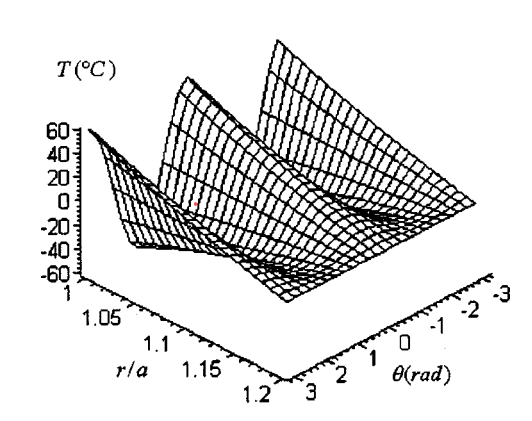
\includegraphics[width=1\textwidth]{example1_fig1.png}
		\caption{Распределение температуры по толщине. К этому я стремлюсь}
	\end{minipage}
	\hfill
	\begin{minipage}[h]{.4\textwidth}
		\centering
		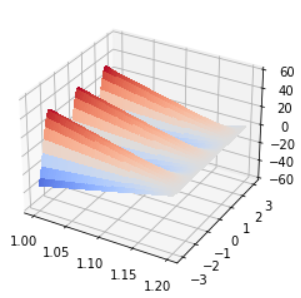
\includegraphics[width=1\textwidth]{example1_fig1b.png}
		\caption{Распределение температуры по толщине. Пока выходит так}
	\end{minipage}
\end{figure}

\begin{figure}[ht]
	\begin{minipage}[h]{.4\textwidth}
		\centering
		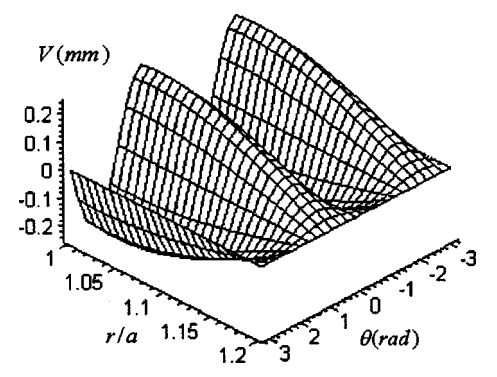
\includegraphics[width=1\textwidth]{example1_fig2.png}
		\caption{Радиальное перемещение по толщине}
	\end{minipage}
	\hfill
	\begin{minipage}[h]{.4\textwidth}
		\centering
		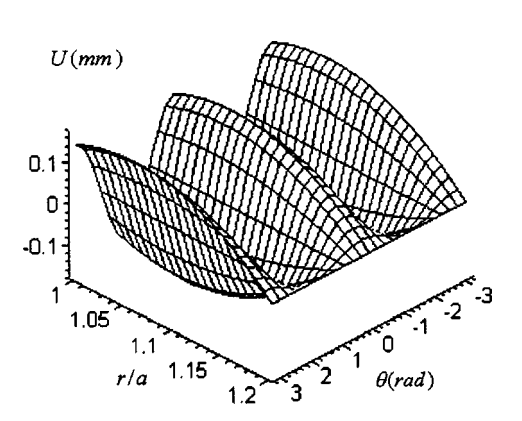
\includegraphics[width=1\textwidth]{example1_fig2a.png}
		\caption{Окружное перемещение по толщине}
	\end{minipage}
\end{figure}

\begin{figure}[ht]
	\begin{minipage}[h]{.4\textwidth}
		\centering
		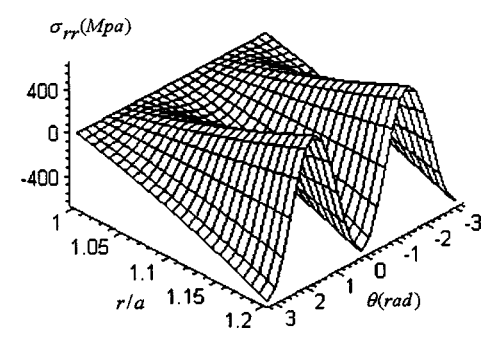
\includegraphics[width=1\textwidth]{example1_fig3a.png}
		\caption{Радиальное термальное напряжениепо толщине}
	\end{minipage}
	\hfill
	\begin{minipage}[h]{.4\textwidth}
		\centering
		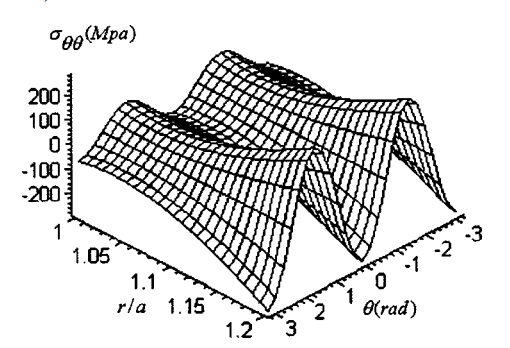
\includegraphics[width=1\textwidth]{example1_fig3b.png}
		\caption{Окружное термальное напряжениепо толщине}
	\end{minipage}
	\hfill
\begin{minipage}[h]{.4\textwidth}
	\centering
	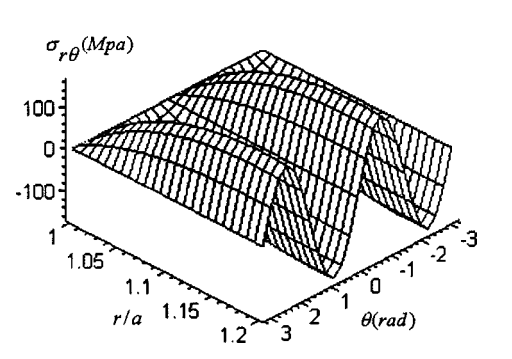
\includegraphics[width=1\textwidth]{example1_fig3c.png}
	\caption{Сдвиговое термальное напряжениепо толщине}
\end{minipage}
\end{figure}  	 % пример для предыдущей главы
\printbibliography[section=0,title=\bibtitlefull]
\end{document}
